 \documentclass{article}
\usepackage{tikz}
\usetikzlibrary{angles, quotes}
\usepackage{amssymb}
\usepackage{pgfplots}
\pgfplotsset{width=10cm,compat=1.9}
\usepgfplotslibrary{statistics}
\usepackage[left=2.54cm,right=2.54cm,top=2.54cm,bottom=2.54cm]{geometry}
\usepackage{tasks} %Paquete necesario para la producción de items horizontales para algunos ejercicios de tarea empleando el comando /begin{multicols}}{#}.../end{multicols} para ayudarnos a reducir las páginas
\usepackage{pdflscape} %comando que permite cambiar a orientación horizontal las hojas%
\usepackage{soul} %Paquete para permitir la compilación de acentos usando el comando {\hl{}}}\\
\sethlcolor{yellow(munsell)} %comando para definir el color para el subrayado usando el comando \hl
\usepackage[utf8]{inputenc}
\usepackage[spanish]{babel}
\usepackage{icomma}
\usepackage{ragged2e}
\usepackage{siunitx}
\usepackage{url}
\usepackage[colorlinks=true, urlcolor=blue,  linkcolor=black, citecolor=green]{hyperref}
\usepackage{pdfpages}
\usepackage{blindtext} %Paquete que genera texto ficticio (dummy text) con el comando: \blindtext
\usepackage{cancel} %in the preamble gives you four different modes of striking through: \cancel{text to cancel} draws a diagonal line (slash) through its argument, \bcancel{text to cancel} uses the negative slope (a backslash), \xcancel{text to cancel} draws an X (actually \cancel plus \bcancel), \cancelto{〈value〉}{〈expression〉} draws a diagonal arrow through the 〈expression〉pointing to the 〈value〉 (math-mode only)
\usepackage{csquotes}
\usepackage{afterpage}
\usepackage{parskip} 
\usepackage{float}
\usepackage{enumitem}
\usepackage{multicol}%Paquete que permite la creación aislada de columnas de texto. De esta forma se reduce la cantidad de páginas en nuestro documento
\usepackage{lipsum} %Paquete que genera texto de relleno al igual que \usepackage{blindtext}, se usa con el comando \lipsum[#-#] los #(hashtags) delimitan el número de páginas que deseamos ocupar del paquete lipsum para usarlos como relleno. 

% Definir el comando personalizado para la nota
\newcommand{\mynote}[1]{%
\begin{tikzpicture}[baseline=-0.75ex]
\node[draw, circle, fill=Apple Green!60, inner sep=2pt] (note) {\textbf{Nota:}};
\end{tikzpicture}%
\ \textit{#1}%
}

\newenvironment{Figura}
{\par\medskip\noindent\minipage{\linewidth}}
{\endminipage\par\medskip}
\usepackage{caption}
\usepackage[
backend=biber,
sorting=none,
url=true
]{biblatex} %bibliografía
\addbibresource{biblio.bib}
% Establecer el espacio entre las entradas de la bibliografía
\setlength{\bibitemsep}{1\baselineskip} % Puedes ajustar el valor según tus preferencias
\usepackage{amsmath,amsthm,amssymb,amsfonts}
\usepackage{pifont} %Permite la compilación del comando \xmark: es el símbolo de la tachita
\usepackage{mathtools} %permite la compilación de símbolos para matrices
\usepackage{empheq} %Paquete que se relaciona con \usepackage[most]{tcolorbox} para la creación de cuadros/cajas de colores para delimitar los resultados matemáticos o líneas de texto usando la línea de comando: \begin{empheq}[box={\mymath[colback=orange(webcolor)!70,drop lifted shadow]}]{equation*} \end{empheq}
\usepackage[most]{tcolorbox} %Paquete que se relaciona con \usepackage{empheq} para la creación de cuadros/cajas de colores para delimitar los resultados matemáticos o líneas de texto
\renewcommand{\qedsymbol}{$\blacksquare$}
\usetikzlibrary{positioning,decorations.pathreplacing} %Paquete que permite la compilación de llaves para cuadros sinópticos (brace diagram) 
\usepackage{schemata} %The schemata package is designed just for these brace diagrams
\usepackage{booktabs}

\newcommand\AB[2]{\schema{\schemabox{#1}}{\schemabox{#2}}} %comando o paquete necesario para crear cuadros sinópticos

\newtcbox{\mymath}[1][]{%
nobeforeafter, math upper, tcbox raise base,
enhanced, colframe=blue!30!black,
colback=blue!30, boxrule=1pt,
#1} %Comando importante para encasillar los resultados matemáticos en cajas de diferentes colores, se relaciona con los paquetes \usepackage{empheq} y \usepackage[most]{tcolorbox} 

\newenvironment{sysmatrix}[1]
{\left(\begin{array}{@{}#1@{}}}
{\end{array}\right)}
\newcommand{\ro}[1]{%
\xrightarrow{\mathmakebox[\rowidth]{#1}}%
}
\newlength{\rowidth}% row operation width
\AtBeginDocument{\setlength{\rowidth}{3em}}  %Comando importante para laproducción de lineas de operaciones entre matrices, método de Gauss o Gauss Jordan se relaciona con \newenvironment{sysmatrix}

%formato para cambiar el horario a español
\usepackage[spanish]{datetime2}
\DTMsetdatestyle{spanish}

\renewcommand{\today}{\DTMdisplaydate{\the\year}{\the\month}{\the\day }{-1}}
%%%%%%%%%%%%%%%%%%%%%%%%%%%%%%%%%%%%%%%%%

\usepackage{datetime}
\newcommand{\mycurrenttime}{\xxivtime}

%%%%%%%%%%%%%%%%%%%%%%%%%%%%%%%%%%%%%%%%%%%%%%%%%%%%%%%%%%%%%%%%%%%%%%%%%%%%%%%%%%%%%%%%%%%%%%%%%%%%%%%%%%%%%%%%%%%%%%%%%%%%%%%%%%%%%%%%%%%%%%%%%


%%%%%%%%%%%%%Caja de color para el título%%%%%%%%%%%%%%%%%%%%%%%%%%%%%%%%%%%%%%%%%%%%%%%%%%%%%%

\definecolor{myframecolor}{RGB}{1, 45, 75} % Prussian Blue
\definecolor{myboxcolor}{RGB}{0, 107, 92} % Apple Green

\newtcolorbox{mybox}{
enhanced,
colback=myboxcolor!7, % Color de fondo del cuadro
colframe=myframecolor, % Color del marco del cuadro
arc=0pt,
boxrule=1pt,
borderline west={2mm}{-10mm}{myframecolor}, % Borde en el lado izquierdo
sharp corners=southwest,
width=\linewidth,
before=\par\vspace{\bigskipamount}, % Espacio antes del cuadro
after=\par\vspace{\bigskipamount} % Espacio después del cuadro
}


\newcommand{\euler}{e} %Comando para producir letra e de euler
\newenvironment{remark}{\par\vfill\footnotesize % Vertical white space above the remark and smaller font size
\begin{list}{}{
	\leftmargin=80pt % Indentation on the left
	\rightmargin=60pt}\item\ignorespaces % Indentation on the right
\makebox[-2.5pt]{\begin{tikzpicture}[overlay]
		\node[draw=Horizon!60,line width=2.5pt,circle,fill=Horizon!25,font=\sffamily\bfseries,inner sep=4pt,outer sep=0pt] at (-19pt,5pt){\textcolor{Horizon}{Nota}};\end{tikzpicture}} % Blue Nota in a circle
\advance\baselineskip -1pt}{\end{list}\vskip5pt} % Tighter line spacing and white space after remark
\usepackage{graphicx}

\usepackage{titling}

\input{colores.tex}

%%Producir signos de cita textual``Asignatura''

\newcommand{\xmark}{\ding{55}} %%%comando que genera la tachita

\newenvironment{MyColorPar}[1]{%
\leavevmode\color{#1}\ignorespaces%
}{%
}%

%%%%%%%%%%%%%%%%%%% Título de la tarea, Nombre de alumno

\title{Problemas  - \textcolor{Tarawera}{\textbf{Segundo parcial}}}
\author{\emph{Julio Alfredo Ballinas García} $\boldsymbol{\mid}$ 202107583}
\date{\today}

%%%%%%%%%%%%%%%%%%% Datos de la Materia

\usepackage{fancyhdr}
\fancypagestyle{plain}{%  the preset of fancyhdr 
\fancyhf{} % clear all header and footer fields
\fancyfoot[R]{
\includegraphics[width=2cm]{LogoFCFMBUAP (1).png}}
\fancyfoot[L]{{\bfseries{\thedate{}}} a las {\bfseries{\mycurrenttime{}}} horas{} (GMT-6, H. Puebla de Zaragoza, Pue)}
\fancyhead[L]{Electrodinámica}
\fancyhead[R]{\theauthor}
}
\makeatletter
\def\@maketitle{%
\newpage
\null
\vskip 1em%
\begin{center}%
\let \footnote \thanks
{\LARGE \@title \par}%
\vskip 1em%
%{\large \@date}%
\end{center}%
\par
\vskip 1em}
\makeatother

\usepackage{lipsum}  
\usepackage{cmbright}


%%%%%%%%%%%%%%%%%%%%%%%%%%%%%%%%%%%%%%%%%%%%%%%%%%%%%%%%%%%%%%%%%%%%%%%%%%%%%%%%%%%%%%%%%%%%%%%%%%%%%%%%%%%%%%%%%%%%%%%%%%%%%%%%%%%%%%%%%%%%%%%%%%%%%%%%%%%%%%%%%%%%%%%%%%%%%%%%%%%%%%%%%%%%%%%%%%%%%%

\begin{document}



\maketitle


%%%%%%%%%%%%%%%%%%% Datos del profesor, campus y aula

\begin{mybox}
\noindent\begin{tabular}{@{}ll}
	{\bfseries{Profesor}} & Dr. Iván Fuentecilla Cárcamo\\
	\textcolor{prussianblue}{\bfseries{Campus}} / \textcolor{trueblue}{\bfseries{Facultad}}  & \textcolor{prussianblue}{\bfseries{C.U. BUAP}} /  \textcolor{trueblue}{\bfseries{FCFM}} \\
	\textcolor{prussianblue}{\bfseries{Edificio}} /  \textcolor{trueblue}{\bfseries{Salón}}    & 	\textcolor{prussianblue}{\bfseries{EMA4}} /  \textcolor{trueblue}{\bfseries{409}}   
\end{tabular} 
\end{mybox} \vspace{1cm}

\section*{\textcolor{Apple Green}{\textbf{Problemas: segundo parcial}}}
\addcontentsline{toc}{section}{\textcolor{Apple Green}{\textbf{Problemas: segundo parcial}}}

%=================== Problema 1 ===================
\begin{enumerate}[label={{\textcolor{trueblue}{\textbf{Pr.} \arabic*.1}}}, start=1]
\item \textbf{A sphere of radius $R$ carries a polarization}

\[
\mathbf{P}(r) = k r,
\]

where $k$ is a constant and $r$ is the vector from the center.

(a) Calculate the bound charges $\sigma_{b}$ and $\rho_{b}$.  
(b) Find the field inside and outside the sphere.
\end{enumerate}

%=================== Problema 2 ===================
\begin{enumerate}[label={{\textcolor{trueblue}{\textbf{Pr.} \arabic*.2}}}]
\item A short cylinder, of radius $a$ and length $L$, carries a ``frozen-in'' uniform polarization $\mathbf{P}$, parallel to its axis. Find the bound charge, and sketch the electric field (i) for $L \gg a$, (ii) for $L \ll a$, and (iii) for $L \approx a$.

[This is known as a \textbf{bar electret}; it is the electrical analog to a bar magnet. In practice, only very special materials—barium titanate is the most “familiar” example—will hold a permanent electric polarization.]
\end{enumerate}

%=================== Problema 3 ===================
\begin{enumerate}[label={{\textcolor{trueblue}{\textbf{Pr.} \arabic*.3}}}]
\item A very long cylinder, of radius $a$, carries a uniform polarization $\mathbf{P}$ perpendicular to its axis. Find the electric field inside the cylinder. Show that the field outside the cylinder can be expressed in the form

\[
\mathbf{E}(r) = \frac{a^{2}}{2\epsilon_{0}s^{2}} \left[ 2(\mathbf{P}\cdot\hat{s})\hat{s} - \mathbf{P} \right].
\]
\end{enumerate}

%=================== Problema 4 ===================
\begin{enumerate}[label={{\textcolor{trueblue}{\textbf{Pr.} \arabic*.4}}}]
\item A thick spherical shell (inner radius $a$, outer radius $b$) is made of dielectric material with a “frozen-in’’ polarization

\[
\mathbf{P}(r) = \frac{k}{r}\,\hat{\mathbf{r}},
\]

where $k$ is a constant and $r$ is the distance from the center (see figure 1). (There is no free charge in the problem.) Locate all the bound charge, and use Gauss’s law to calculate the field it produces.

\begin{center}
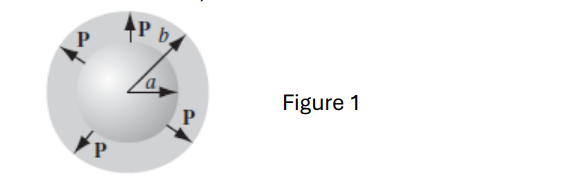
\includegraphics[width=0.85\linewidth]{FIGURA_1.png} % <-- Sustituye esta ruta
\\[2mm]
\textbf{Figure 1}
\end{center}

\end{enumerate}

%=================== Problema 5 ===================
\begin{enumerate}[label={{\textcolor{trueblue}{\textbf{Pr.} \arabic*.5}}}]
\item Suppose you have enough linear dielectric material, of dielectric constant $\epsilon_{r}$, to half-fill a parallel-plate capacitor (see figure 2). By what fraction is the capacitance increased when you distribute the material as in the figure 2 (a)? How about Figure 2 (b)? For a given potential difference $V$ between the plates, find $\mathbf{E}$, $\mathbf{D}$, and $\mathbf{P}$, in each region, and the free and bound charge on all surfaces, for both cases.

\begin{center}
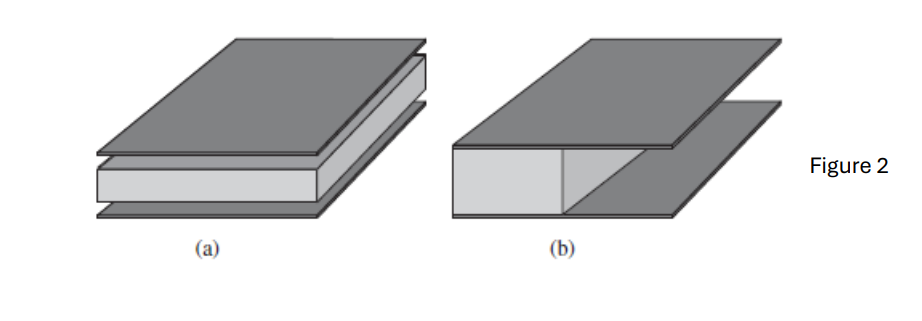
\includegraphics[width=0.95\linewidth]{FIGURA_2.png} % <-- Sustituye con imagen (a) y (b)
\\[2mm]
\textbf{Figure 2}
\end{center}

\end{enumerate}

%=================== Problema 6 ===================
\begin{enumerate}[label={{\textcolor{trueblue}{\textbf{Pr.} \arabic*.6}}}]
\item An uncharged conducting sphere of radius $a$ is coated with a thick insulating shell (dielectric constant $\epsilon_{r}$) out to radius $b$. This object is now placed in an otherwise uniform electric field $\mathbf{E}_{0}$. Find the electric field in the insulator.
\end{enumerate}

%=================== Problema 7 ===================
\begin{enumerate}[label={{\textcolor{trueblue}{\textbf{Pr.} \arabic*.7}}}]
\item A dielectric cube of side $a$, centered at the origin, carries a “frozenin’’ polarization $\mathbf{P} = k r$, where $k$ is a constant. Find all the bound charges, and check that they add up to zero.
\end{enumerate}

%=================== Problema 8 ===================
\begin{enumerate}[label={{\textcolor{trueblue}{\textbf{Pr.} \arabic*.8}}}]
\item Use the Clausius-Mossotti equation to determine the polarizability of atoms in the air molecules: $\mathrm{N}_{2}$, $\mathrm{O}_{2}$. Determine the average radius of the atom in an air molecule.
\end{enumerate}

%=================== Problema 9 ===================
\begin{enumerate}[label={{\textcolor{trueblue}{\textbf{Pr.} \arabic*.9}}}]
\item Figure 3 shows a simple cubic lattice of molecules all of which have the same (in direction and magnitude) dipole moment $p_{m}$. Let us fix our attention on one particular molecule, call it $j$. It is evident that $j$ has six nearest neighbors at distance $a$, twelve next-nearest neighbors at distance $\sqrt{2}\, a$, etc. Find the electric field at $j$ due to the six $p_{m}$ on nearest-neighbor molecules for an arbitrary orientation of $p_{m}$. (Let the lines joining $j$ to its nearest neighbors define the $x,y$ and $z$-axes. For simplicity, take $p_{m}$ in the $xz$-plane, making an angle $\theta$ with the $x$-axis.)

\begin{center}
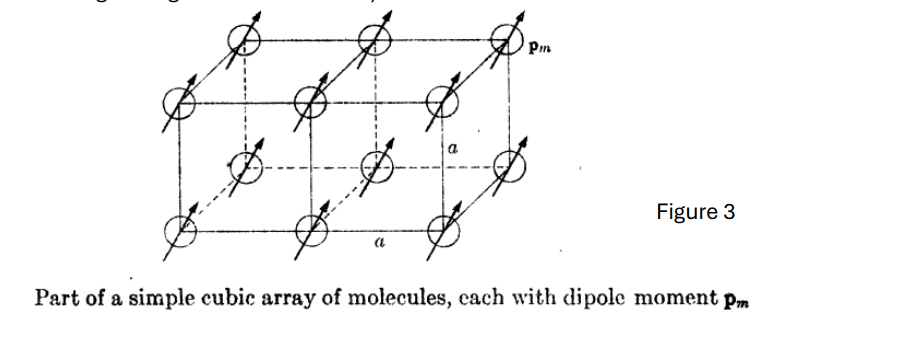
\includegraphics[width=0.95\linewidth]{FIGURA_3.png} % <-- Sustituye esta ruta
\\[2mm]
\textbf{Figure 3}
\end{center}

\end{enumerate}

%=================== Problema 10 ===================
\begin{enumerate}[label={{\textcolor{trueblue}{\textbf{Pr.} \arabic*.10}}}]
\item A fast electron (kinetic energy = $3.0 \times 10^{-17}$ joule) enters a region of space containing a uniform electric field $E = 1000$ volts/m. The field is parallel to the electron’s motion, and in a direction such as to decelerate it. How far does the electron travel before it is brought to rest?
\end{enumerate}

%=================== Problema 11 ===================
\begin{enumerate}[label={{\textcolor{trueblue}{\textbf{Pr.} \arabic*.11}}}]
\item Given a spherical dielectric shell (inner radius $a$, outer radius $b$, dielectric constant $K$) and a point charge $q$, infinitely separated. Now let the point charge be placed at the center of the dielectric shell. Determine the change in energy of the system.
\end{enumerate}

%=================== Problema 12 ===================
\begin{enumerate}[label={{\textcolor{trueblue}{\textbf{Pr.} \arabic*.12}}}]
\item Given a spherical charge distribution of radius $R$, uniform charge density $\rho_{0}$. Determine the self-energy of the distribution in two ways:  
(a) by direct integration;  
(b) by an integration over the field,
\[
\frac{1}{2} \int \mathbf{E}\cdot \mathbf{D}\, dv.
\]
\end{enumerate}




\tableofcontents \newpage

\begin{center}
\begin{tikzpicture}
	% Dibuja círculos rellenos en diferentes colores
	\fill[bittersweet] (0,0) circle (0.17cm);
	\fill[Apple Green] (0.6,0) circle (0.17cm);
	\fill[trueblue] (1.2,0) circle (0.17cm);
	\fill[Aguamarina] (1.8,0) circle (0.17cm);
	\fill[Sun] (2.4,0) circle (0.17cm);
	\fill[orange(colorwheel)] (3.0,0) circle (0.17cm);
	\fill[Pesto] (3.6,0) circle (0.17cm);
	\fill[blue-violet] (4.2,0) circle (0.17cm);
	\fill[ticklemepink] (4.8,0) circle (0.17cm);
	\fill[Gallery] (5.4,0) circle (0.17cm);
	\fill[Mantle] (6.0,0) circle (0.17cm);
	\fill[Nevada] (6.6,0) circle (0.17cm);
	\fill[onyx] (7.2,0) circle (0.17cm);
	% Agrega más círculos o modifica los colores según sea necesario
\end{tikzpicture}
\end{center}  \vspace{2cm}


\section{Problema 1}

\textcolor{Cinnabar}{\textbf{Solución Pr. 1.1}} \vspace{0.4cm}

El sistema es una esfera de radio $R$ con una polarización que depende linealmente de la posición,
\begin{equation}
\mathbf{P}(\mathbf{r}) = k\,\mathbf{r}
\label{eq:P-kr-esfera}
\end{equation}
donde $k$ es una constante escalar y $\mathbf{r}$ es el vector de posición medido desde el centro de la esfera

\subsubsection*{(a) Cargas ligadas $\rho_{b}$ y $\sigma_{b}$}

En un dieléctrico polarizado, las densidades de \textbf{carga ligada} se obtienen a partir de la polarización mediante
\begin{align}
\rho_{b} &= - \nabla \cdot \mathbf{P}
\quad \text{(densidad de carga ligada de volumen)} 
\label{eq:rho-b-def} \\
\sigma_{b} &= \mathbf{P}\cdot \hat{\mathbf{n}}
\quad \text{(densidad de carga ligada superficial)}
\label{eq:sigma-b-def}
\end{align}
donde $\hat{\mathbf{n}}$ es el vector normal unitario \emph{saliente} a la superficie


\paragraph{Densidad volumétrica $\rho_{b}$}

Usando \eqref{eq:P-kr-esfera} en \eqref{eq:rho-b-def},
\begin{equation}
\nabla \cdot \mathbf{P} = \nabla \cdot (k\,\mathbf{r}) = k\,\nabla \cdot \mathbf{r}
\label{eq:div-P-paso1}
\end{equation}
En coordenadas cartesianas $\mathbf{r} = x\,\hat{\mathbf{x}} + y\,\hat{\mathbf{y}} + z\,\hat{\mathbf{z}}$, de modo que
\begin{equation}
\nabla \cdot \mathbf{r} = 
\frac{\partial x}{\partial x} +
\frac{\partial y}{\partial y} +
\frac{\partial z}{\partial z} = 1 + 1 + 1 = 3
\label{eq:div-r}
\end{equation}
Sustituyendo \eqref{eq:div-r} en \eqref{eq:div-P-paso1},
\begin{equation}
\nabla \cdot \mathbf{P} = 3k
\label{eq:div-P-final}
\end{equation}
Por tanto,
\begin{equation}
\rho_{b} = - \nabla \cdot \mathbf{P} = -3k
\label{eq:rho-b-final}
\end{equation}
Es decir, dentro de la esfera la densidad de carga ligada de volumen es \textbf{constante} e igual a $-3k$

\paragraph{Densidad superficial $\sigma_{b}$}

La carga ligada superficial vive únicamente en la superficie esférica $r = R$. Ahí, la normal saliente es radial,
\begin{equation}
\hat{\mathbf{n}} = \hat{\mathbf{r}}
\label{eq:n-hat}
\end{equation}
En la superficie, la polarización vale
\begin{equation}
\mathbf{P}(R) = k\,\mathbf{r}\big|_{r = R} = kR\,\hat{\mathbf{r}}
\label{eq:P-en-R}
\end{equation}
Aplicando \eqref{eq:sigma-b-def},
\begin{equation}
\sigma_{b} = \mathbf{P}\cdot \hat{\mathbf{n}} = \mathbf{P}(R)\cdot \hat{\mathbf{r}} = kR
\label{eq:sigma-b-final}
\end{equation}
Por tanto,
\begin{equation}
\rho_{b} = -3k \quad \text{para } r < R,
\qquad
\sigma_{b} = kR \quad \text{en } r = R
\label{eq:rho-sigma-resumen}
\end{equation}

Como verificación, calculemos la carga ligada total.  
La carga ligada de volumen es
\begin{equation}
Q_{b}^{(\text{vol})} 
= \int_{V} \rho_{b}\, dV
\quad \text{donde } dV \text{ es el elemento de volumen}
= (-3k)\left(\frac{4\pi R^{3}}{3}\right)
= -4\pi k R^{3}
\label{eq:Qb-vol}
\end{equation}

La carga ligada superficial es
\begin{equation}
Q_{b}^{(\text{sup})} 
= \int_{S} \sigma_{b}\, dA
\quad \text{donde } dA \text{ es el elemento de área sobre la superficie}
= (kR)(4\pi R^{2})
= 4\pi k R^{3}
\label{eq:Qb-sup}
\end{equation}

Entonces,
\begin{equation}
Q_{b}^{\text{(total)}} 
= Q_{b}^{(\text{vol})} + Q_{b}^{(\text{sup})} 
= -4\pi k R^{3} + 4\pi k R^{3}
= 0
\label{eq:Qb-total}
\end{equation}

La esfera polarizada es globalmente neutra, como es de esperarse.



\subsubsection*{(b) Campo eléctrico dentro y fuera de la esfera}

Usamos la ley de Gauss en forma integral,
\begin{equation}
\oint_{S} \mathbf{E}\cdot d\mathbf{A} = \frac{1}{\epsilon_{0}}\,Q_{\text{enc}}
\label{eq:gauss}
\end{equation}
donde $Q_{\text{enc}}$ es la carga \emph{ligada} encerrada por la superficie gaussiana
(no hay carga libre en el problema) y $d\mathbf{A}$ es el vector área sobre la superficie cerrada $S$.

Por simetría esférica, el campo eléctrico es radial y sólo depende de $r$:
\begin{equation}
\mathbf{E}(\mathbf{r}) = E(r)\,\hat{\mathbf{r}}
\label{eq:E-radial}
\end{equation}

\paragraph{Campo para $r < R$ (interior de la esfera)}

Tomemos como superficie gaussiana una esfera de radio $r<R$ centrada en el origen.  
Dentro de esta esfera sólo se encierra la carga ligada de volumen. Entonces,
\begin{equation}
Q_{\text{enc}}(r) = \int_{V_{r}} \rho_{b}\, dV
\quad \text{donde } V_{r} \text{ es la esfera de radio } r
\label{eq:Qenc-def}
\end{equation}
En este problema $\rho_{b}$ es constante en el interior, $\rho_{b} = -3k$, así que
\begin{equation}
Q_{\text{enc}}(r) = \rho_{b}\int_{V_{r}} dV
= \rho_{b}\, \text{Volumen}(\text{esfera de radio } r)
\label{eq:Qenc-rho-const}
\end{equation}
El volumen de una esfera de radio $r$ puede obtenerse integrando explícitamente en coordenadas esféricas,
\[
dV = r'^{2}\sin\theta\,dr'\,d\theta\,d\varphi
\]
\[
\int_{V_{r}} dV
= \int_{0}^{r}\int_{0}^{\pi}\int_{0}^{2\pi}
r'^{2}\sin\theta\,d\varphi\,d\theta\,dr'
= \int_{0}^{r} r'^{2}dr'
\left(\int_{0}^{\pi}\sin\theta\,d\theta\right)
\left(\int_{0}^{2\pi}d\varphi\right)
\]
\[
= \left[\frac{r'^{3}}{3}\right]_{0}^{r} \cdot (2) \cdot (2\pi)
= \frac{r^{3}}{3}\cdot 4\pi
= \frac{4\pi r^{3}}{3}
\]
Por tanto,
\begin{equation}
Q_{\text{enc}}(r)
= \rho_{b}\,\frac{4\pi r^{3}}{3}
= (-3k)\,\frac{4\pi r^{3}}{3}
= -4\pi k r^{3}
\label{eq:Qenc-r-menor-R}
\end{equation}

Ahora calculamos el flujo de $\mathbf{E}$ a través de la superficie esférica de radio $r$.  
En esa superficie, el campo es radial y de magnitud constante $E(r)$, y
\[
d\mathbf{A} = \hat{\mathbf{r}}\,dA, 
\qquad dA = r^{2}\sin\theta\,d\theta\,d\varphi
\]
Así,
\begin{equation}
\oint_{S} \mathbf{E}\cdot d\mathbf{A}
= \oint_{S} E(r)\,\hat{\mathbf{r}}\cdot\hat{\mathbf{r}}\,dA
= E(r)\oint_{S} dA
= E(r)\,(4\pi r^{2})
\label{eq:flujo-r-menor-R}
\end{equation}

Sustituyendo \eqref{eq:Qenc-r-menor-R} y \eqref{eq:flujo-r-menor-R} en \eqref{eq:gauss},
\begin{equation}
E(r)\,(4\pi r^{2}) = \frac{1}{\epsilon_{0}}\left(-4\pi k r^{3}\right)
\label{eq:gauss-interior-paso}
\end{equation}
Cancelando $4\pi r^{2}$ en ambos lados:
\[
E(r) = -\,\frac{k}{\epsilon_{0}}\,r
\]
es decir,
\begin{equation}
E(r) = -\,\frac{k}{\epsilon_{0}}\,r
\label{eq:E-magn-interior}
\end{equation}
y el vector campo dentro de la esfera queda
\begin{equation}
\mathbf{E}_{\text{in}}(\mathbf{r}) = -\,\frac{k}{\epsilon_{0}}\,r\,\hat{\mathbf{r}}
\qquad (r < R)
\label{eq:E-vector-interior}
\end{equation}
Su magnitud crece linealmente con $r$ y apunta radialmente \emph{hacia el centro} si $k>0$.

\paragraph{Campo para $r > R$ (exterior)}

Para una superficie gaussiana de radio $r>R$, se encierra toda la carga ligada de volumen y de superficie. Pero ya vimos en \eqref{eq:Qb-total} que
\begin{equation}
Q_{\text{enc}}(r>R) = Q_{b}^{\text{(total)}} = 0
\label{eq:Qenc-mayor-R}
\end{equation}
Entonces, por \eqref{eq:gauss},
\begin{equation}
\oint_{S} \mathbf{E}\cdot d\mathbf{A} = 0
\label{eq:gauss-exterior}
\end{equation}
y por simetría sólo es posible que
\begin{equation}
\mathbf{E}_{\text{out}}(\mathbf{r}) = \mathbf{0}
\qquad (r > R)
\label{eq:E-exterior}
\end{equation}

\subsubsection*{Resumen}

\begin{align}
\rho_{b} &= -3k \quad \text{para } r < R \\
\sigma_{b} &= kR \quad \text{en } r = R \\
\mathbf{E}(\mathbf{r}) &= -\,\dfrac{k}{\epsilon_{0}}\,r\,\hat{\mathbf{r}} 
\quad \text{para } r < R \\
\mathbf{E}(\mathbf{r}) &= \mathbf{0} \quad \text{para } r > R
\end{align}


\section{Problema 2}

\begin{center}
    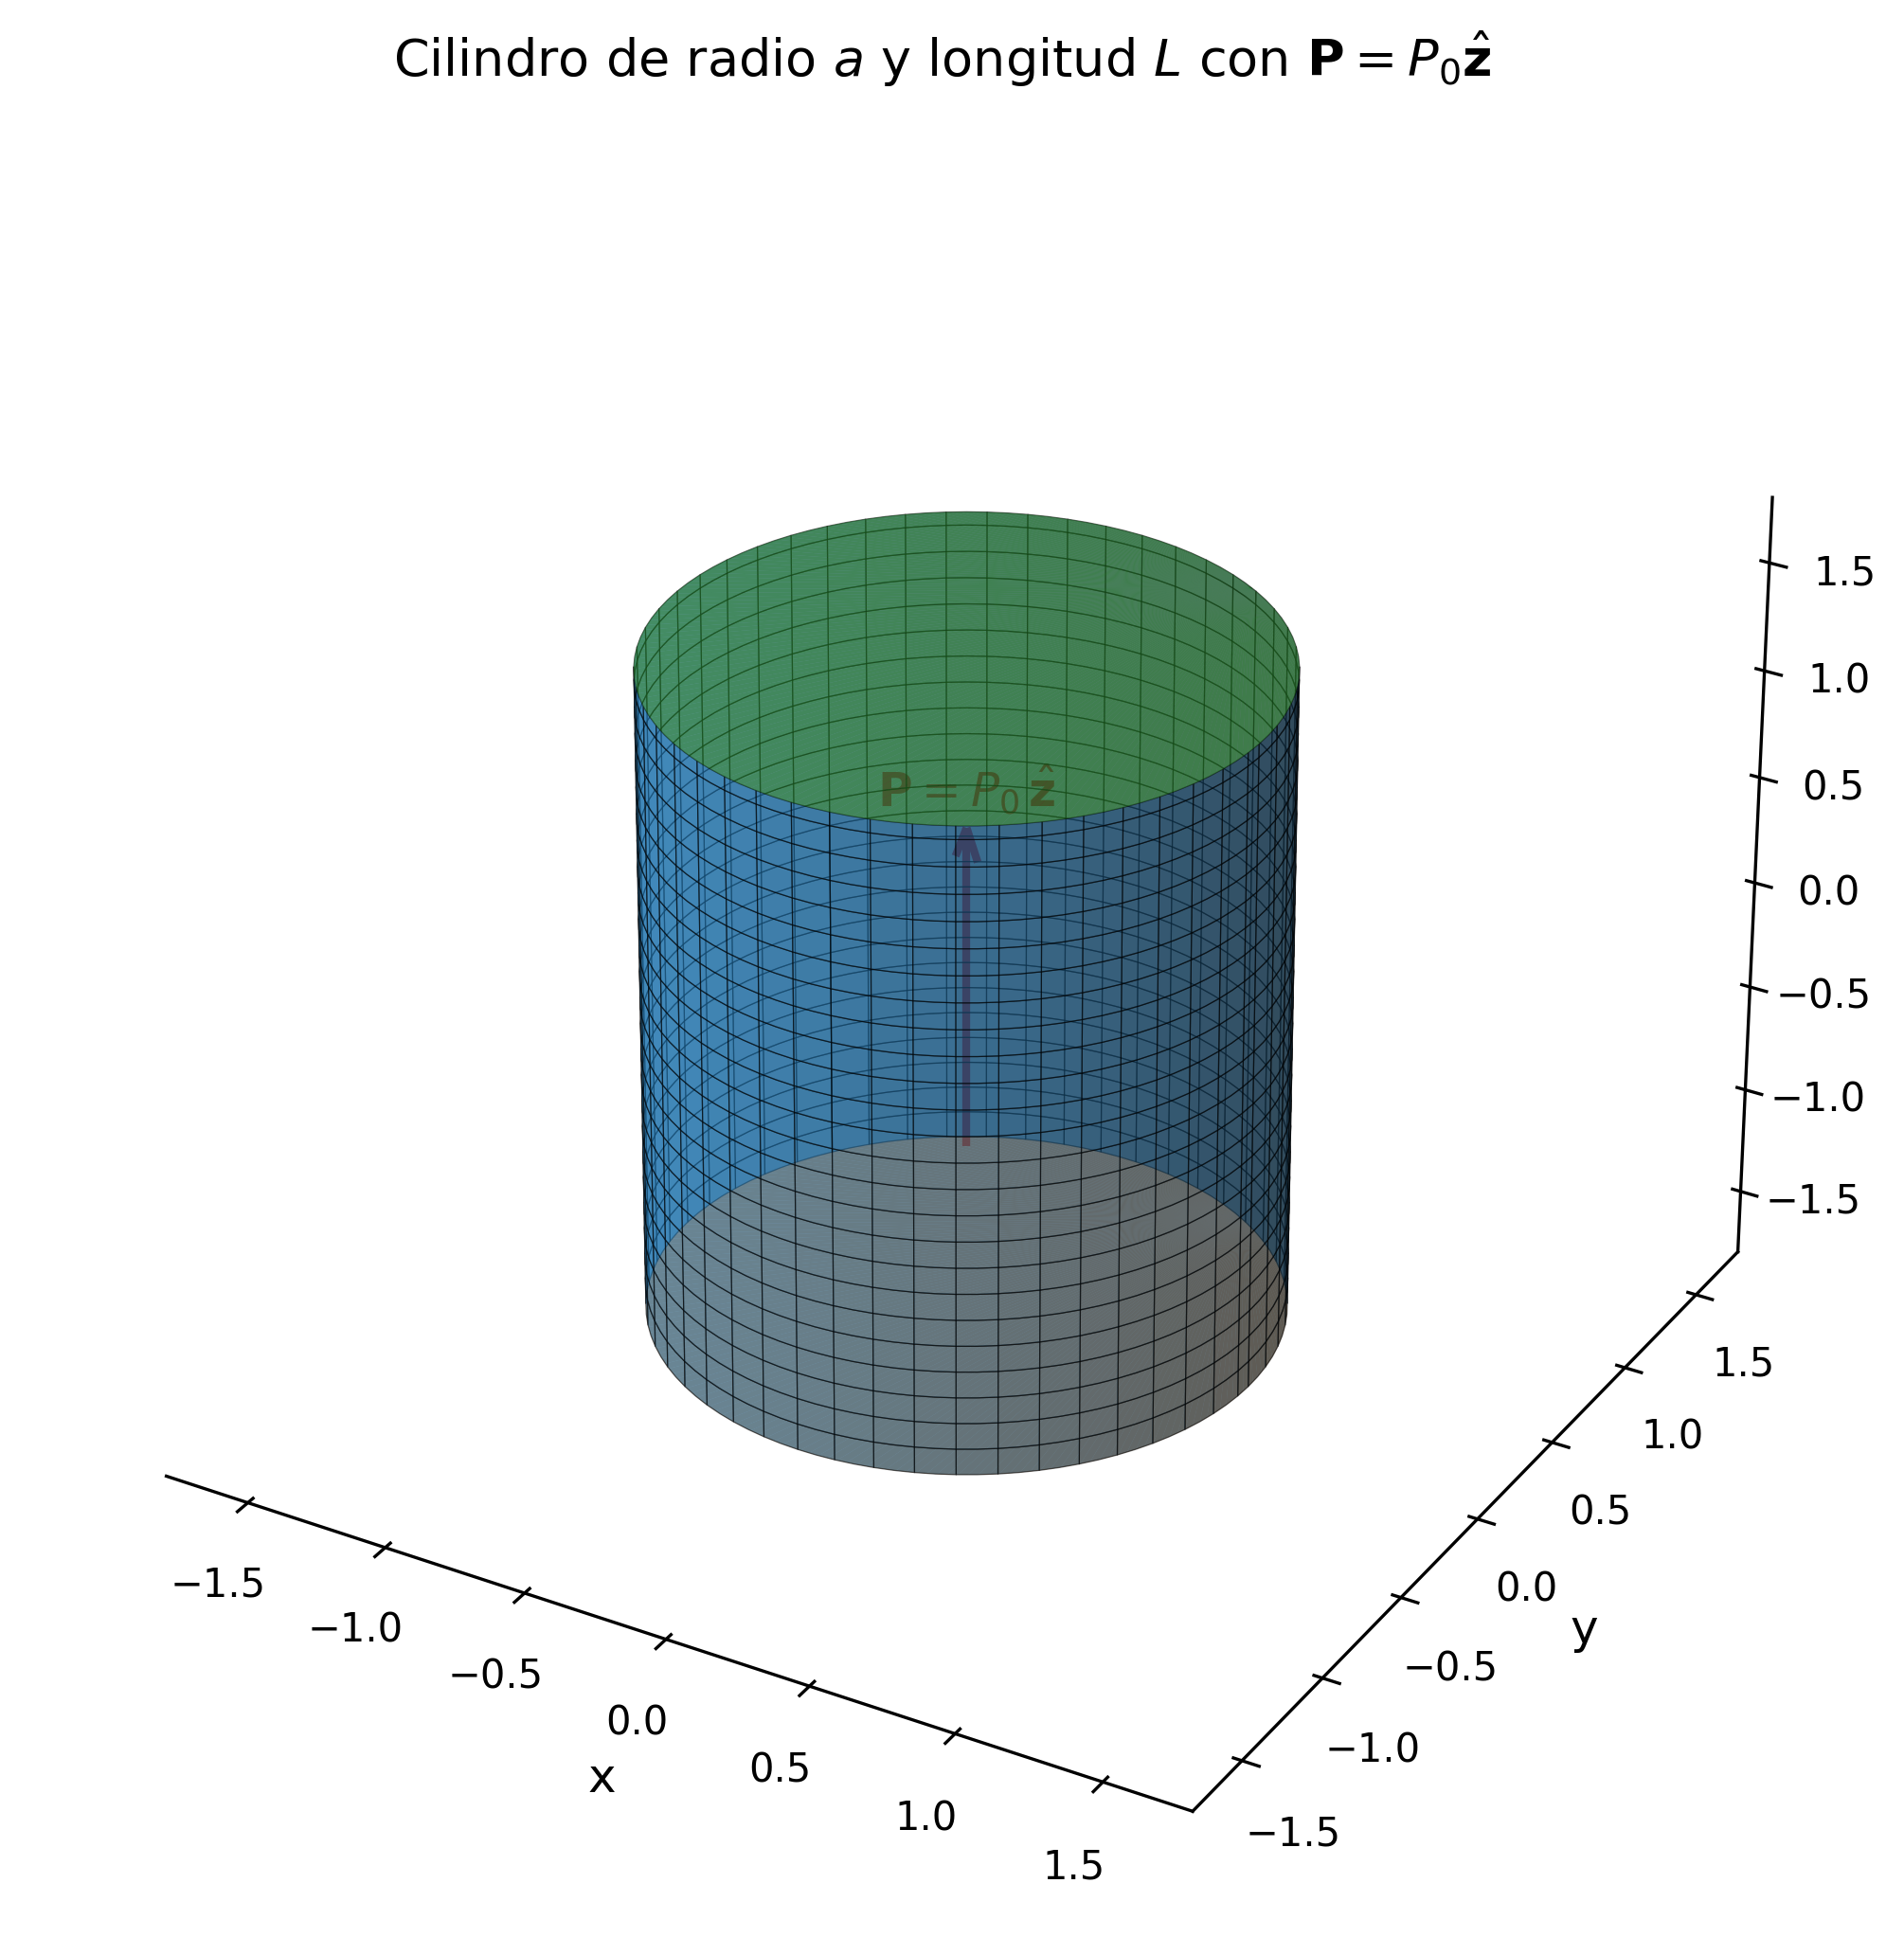
\includegraphics[width=0.6\linewidth]{cilindro_polarizado.png}
    
    \vspace{2mm}
    \small
    \textbf{Figura 1.} Representación geométrica del cilindro de radio $a$ y longitud $L$,
    cuyo eje coincide con el eje $z$, con una polarización ``congelada’’ uniforme
    $\mathbf{P} = P_{0}\,\hat{\mathbf{z}}$ dirigida a lo largo del eje del cilindro.
\end{center}

\textcolor{Cinnabar}{\textbf{Solución Pr. 2.2}} \vspace{0.4cm}

Consideremos un cilindro de radio $a$ y longitud $L$ cuyo eje coincide con el eje $z$. 
El material posee una \emph{polarización ``congelada’’} —es decir, una polarización 
\textbf{permanente, fija dentro del material y no inducida por ningún campo externo}— 
uniforme y dirigida a lo largo del eje del cilindro:
\begin{equation}
\mathbf{P} = P_{0}\,\hat{\mathbf{z}},
\label{eq:P-cilindro-uniforme}
\end{equation}
donde $P_{0}$ es una constante.


\subsubsection*{Cargas ligadas}

Como en el problema anterior, las densidades de \textbf{carga ligada} se obtienen a partir
de la polarización mediante las siguientes relaciones fundamentales:

\begin{align}
\rho_{b} &= -\,\nabla\cdot\mathbf{P}
\label{eq:rho-b-cilindro-def}
\quad\text{(densidad de \emph{carga ligada de volumen})} \\[6pt]
\sigma_{b} &= \mathbf{P}\cdot\hat{\mathbf{n}}
\label{eq:sigma-b-cilindro-def}
\quad\text{(densidad de \emph{carga ligada superficial})}
\end{align}

Aquí:
- $\rho_{b}$ es la carga ligada distribuida dentro del volumen del material,
- $\sigma_{b}$ es la carga ligada que aparece únicamente sobre superficies donde $\mathbf{P}$ tiene componente normal,
- $\hat{\mathbf{n}}$ es el vector normal unitario saliente a la superficie.


\paragraph{Carga de volumen}

La polarización del cilindro es
\[
\mathbf{P} = P_{0}\,\hat{\mathbf{z}},
\]
la cual es \textbf{constante en magnitud y dirección} en todo el volumen.  
Esto significa que:

- no depende de $x$,  
- no depende de $y$,  
- no depende de $z$.  

En notación explícita,
\[
\mathbf{P} = (0, 0, P_{0}),
\]
donde $P_{0}$ es una constante fija.

La divergencia de un campo constante es nula porque las derivadas espaciales de sus componentes son cero:
\[
\nabla\cdot\mathbf{P}
= \frac{\partial P_{x}}{\partial x}
+ \frac{\partial P_{y}}{\partial y}
+ \frac{\partial P_{z}}{\partial z}
= \frac{\partial (0)}{\partial x}
+ \frac{\partial (0)}{\partial y}
+ \frac{\partial (P_{0})}{\partial z}
= 0.
\]

Por lo tanto,
\begin{equation}
\nabla\cdot\mathbf{P} = 0
\label{eq:div-P-cilindro}
\end{equation}
y de la definición
\[
\rho_{b} = -\nabla\cdot\mathbf{P},
\]
obtenemos
\begin{equation}
\rho_{b} = 0.
\label{eq:rho-b-cilindro-final}
\end{equation}

No aparece carga ligada de volumen porque \textbf{no hay variación espacial} de la
polarización dentro del material. Recordemos que la \emph{carga ligada} es la carga
aparente que surge debido a la orientación y distribución de los dipolos en un
dieléctrico: cuando $\mathbf{P}$ cambia de un punto a otro, sus dipolos internos dejan
``“sobrantes’’`` de carga en algunas regiones (lo que produce $\rho_{b}$). Pero si
$\mathbf{P}$ es constante en todo el volumen, los dipolos no dejan ninguna acumulación
netta de carga, de modo que $\rho_{b}=0$ en todo el interior.



\paragraph{Carga superficial}

La carga ligada superficial vive en las superficies laterales y en las dos caras planas del cilindro.  
En la superficie lateral la normal unitara es radial, $\hat{\mathbf{n}} = \hat{\mathbf{s}}$, ortogonal a $\hat{\mathbf{z}}$, por lo que
\begin{equation}
\sigma_{b}^{(\text{lateral})} = \mathbf{P}\cdot\hat{\mathbf{s}} = 0
\label{eq:sigma-b-lateral}
\end{equation}
Así, \textbf{no hay carga ligada} sobre la pared cilíndrica

En las tapas del cilindro, la normal unitaria $\hat{\mathbf{n}}$ es simplemente el 
vector perpendicular a cada cara, apuntando hacia afuera del material. Como el eje 
del cilindro coincide con el eje $z$, las tapas están “planas’’ en planos de $z$ 
constante:

\begin{itemize}
    \item La tapa superior está en $z = +L/2$.
    \item La tapa inferior está en $z = -L/2$.
\end{itemize}

\begin{center}
    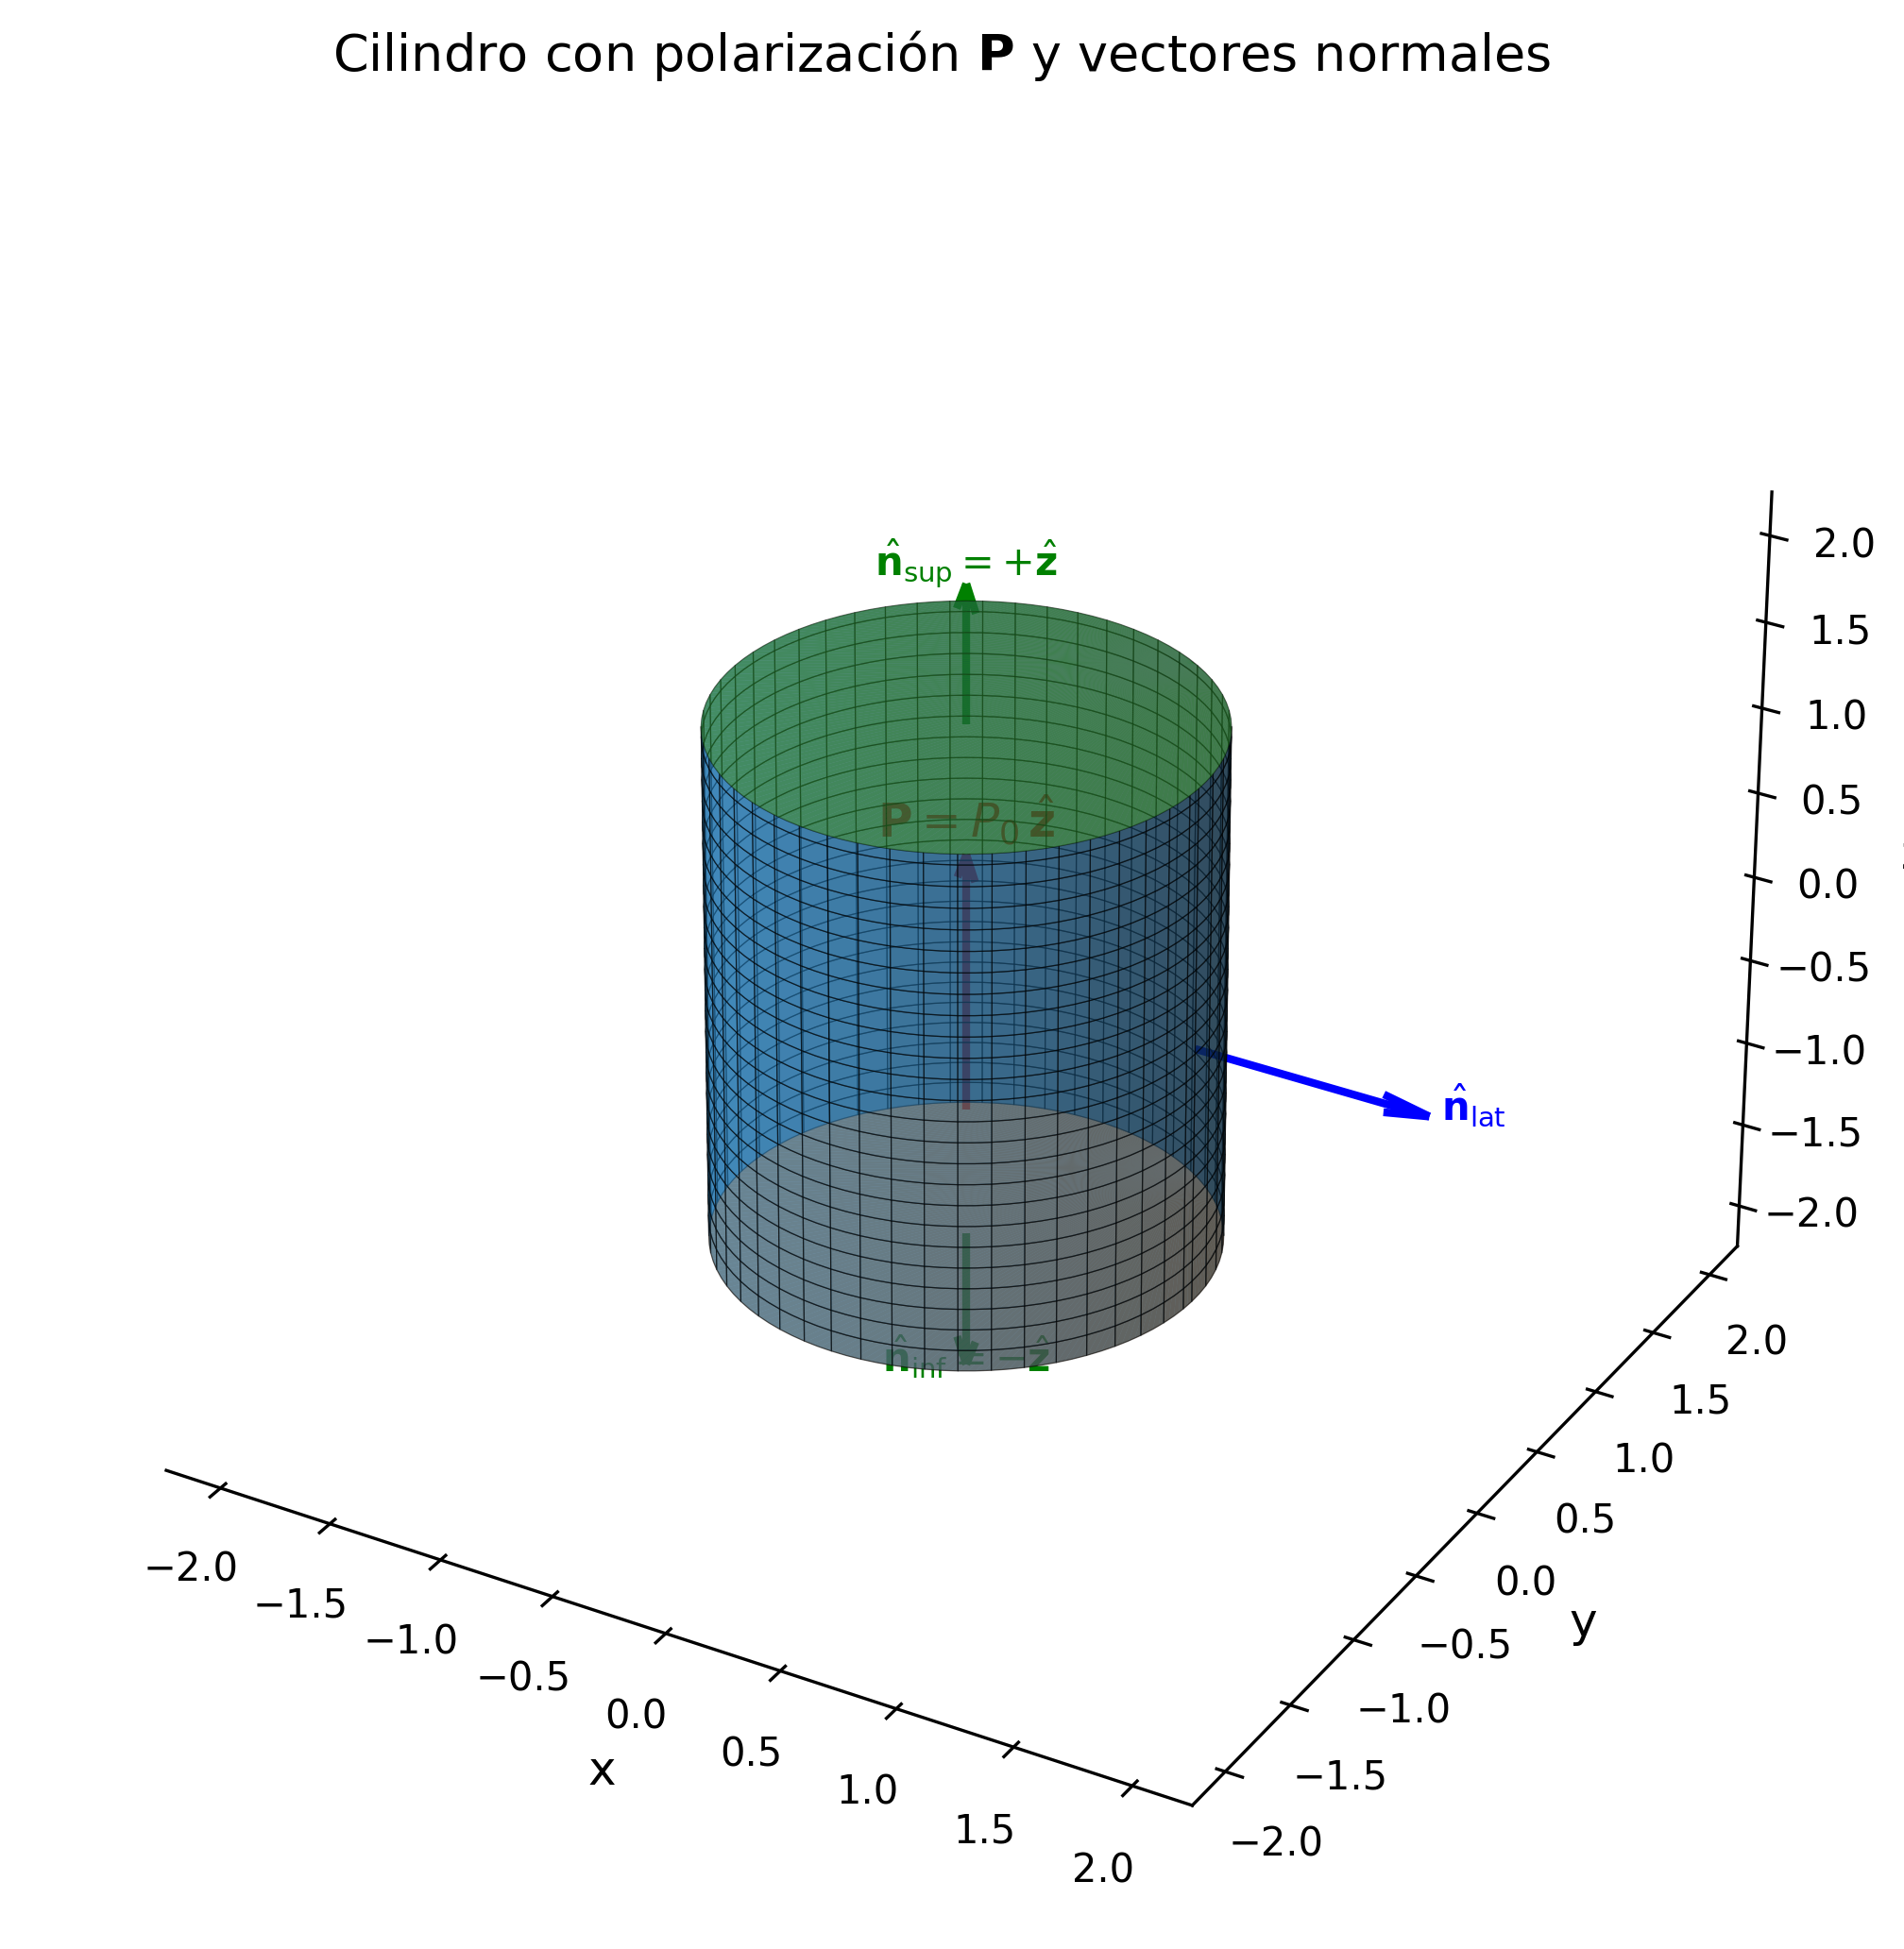
\includegraphics[width=0.70\linewidth]{cilindro_normales.png}

    \vspace{2mm}
    \small
    \textbf{Figura 2.} Representación tridimensional del cilindro de radio $a$ y longitud $L$,
    mostrando la polarización ``congelada'' $\mathbf{P} = P_{0}\hat{\mathbf{z}}$ (flecha roja)
    y las normales unitarias de cada superficie: 
    $\hat{\mathbf{n}}_{\text{sup}} = +\hat{\mathbf{z}}$ en la tapa superior,
    $\hat{\mathbf{n}}_{\text{inf}} = -\hat{\mathbf{z}}$ en la tapa inferior,
    y una normal radial típica $\hat{\mathbf{n}}_{\text{lat}}$ en la superficie lateral del cilindro.
\end{center}


Por convención, la normal unitaria siempre apunta hacia el \emph{exterior} del sólido:

\[
\hat{\mathbf{n}}_{\text{sup}} = +\hat{\mathbf{z}}, 
\qquad
\hat{\mathbf{n}}_{\text{inf}} = -\hat{\mathbf{z}}.
\]

Esto ocurre porque:
\begin{itemize}
    \item En la tapa superior, “hacia afuera’’ es hacia arriba, es decir, en el 
    sentido positivo del eje $z$.
    \item En la tapa inferior, “hacia afuera’’ es hacia abajo, es decir, en el 
    sentido negativo del eje $z$.
\end{itemize}

\noindent
Ahora usamos la definición de carga superficial ligada,
\[
\sigma_{b} = \mathbf{P}\cdot\hat{\mathbf{n}},
\]
junto con la polarización del problema,
\[
\mathbf{P} = P_{0}\,\hat{\mathbf{z}}.
\]

Entonces:

\begin{align}
\sigma_{b}^{(\text{sup})} &= \mathbf{P}\cdot\hat{\mathbf{n}}_{\text{sup}}
= (P_{0}\,\hat{\mathbf{z}})\cdot(+\hat{\mathbf{z}})
= P_{0}, \\[4pt]
\sigma_{b}^{(\text{inf})} &= \mathbf{P}\cdot\hat{\mathbf{n}}_{\text{inf}}
= (P_{0}\,\hat{\mathbf{z}})\cdot(-\hat{\mathbf{z}})
= -P_{0}.
\end{align}

En palabras:

\begin{itemize}
    \item La cara superior presenta una densidad de carga ligada \textbf{positiva},
    porque la polarización apunta “hacia afuera’’ de la superficie.
    \item La cara inferior presenta una densidad de carga ligada \textbf{negativa},
    porque la polarización apunta “hacia adentro’’ (opuesta a la normal).
\end{itemize}

Físicamente, esto representa el hecho de que la polarización 
$\mathbf{P}$ alinea dipolos dentro del material:
el extremo “positivo’’ de cada dipolo queda acumulado en la tapa superior y el 
extremo “negativo’’ en la inferior. Es como si el cilindro fuera un 
\emph{electreto} (el análogo eléctrico de un imán), con “cargas’’ $\pm P_{0}$ 
apareciendo en las caras.

Por eso la situación se asemeja a dos discos paralelos con densidades 
superficiales opuestas, separadas una distancia $L$.

\subsubsection*{Esbozo del campo eléctrico}

Aunque el problema pide un dibujo, podemos describir el campo en tres regímenes geométricos

\paragraph{(i) Caso $L \gg a$ (cilindro muy largo)}

Cuando la longitud es mucho mayor que el radio:

- Las caras cargadas están muy separadas una de otra  
- Cada cara genera un campo que, cerca de ella, es aproximadamente el de un disco aislado con densidad $\sigma = \pm P_{0}$  
- En la región central, lejos de las tapas, los campos de ambas caras prácticamente no se solapan

Consecuencias:

- En la \textbf{parte media} del cilindro, el campo es muy pequeño, $\mathbf{E} \approx \mathbf{0}$, tanto dentro como fuera  
- Cerca de la cara superior, las líneas de campo salen perpendicularmente de la superficie (como de un disco cargado positivamente)  
- Cerca de la cara inferior, las líneas de campo entran perpendicularmente a la superficie (como hacia un disco cargado negativamente)  
- Lejos del cilindro, el campo total se hace muy pequeño, porque la carga total es nula

En el dibujo, se representarían \emph{manojos} de líneas saliendo de la cara superior y entrando en la inferior, concentradas en regiones cercanas a las tapas

\paragraph{(ii) Caso $L \ll a$ (cilindro muy corto, tipo ``pastilla’’)}

Ahora la distancia entre caras es pequeña comparada con el radio. Las superficies $\pm P_{0}$ forman casi un \emph{capacitor plano} de placas grandes y separación pequeña. En este caso, en la región central:

- El campo entre las placas es aproximadamente uniforme y perpendicular a ellas  
- La magnitud del campo electrostático entre dos planchas infinitas con densidades $\pm\sigma$ es
  \begin{equation}
  E \approx \frac{\sigma}{\epsilon_{0}}
  \label{eq:E-capacitor}
  \end{equation}
  con dirección desde la placa positiva hacia la negativa

Como aquí $\sigma_{b}^{(\text{sup})} = +P_{0}$ y $\sigma_{b}^{(\text{inf})} = -P_{0}$, el campo en el interior, en la zona central, es aproximadamente
\begin{equation}
\mathbf{E}_{\text{in}} \approx -\,\frac{P_{0}}{\epsilon_{0}}\,\hat{\mathbf{z}}
\label{eq:E-interior-corto}
\end{equation}
(apunta del disco superior al inferior, es decir, en dirección $-\hat{\mathbf{z}}$ si $P_{0} > 0$)

Fuera del cilindro, los campos de las dos superficies se cancelan casi por completo, de modo que
\begin{equation}
\mathbf{E}_{\text{out}} \approx \mathbf{0}
\label{eq:E-exterior-corto}
\end{equation}
excepto en las inmediaciones del borde, donde aparecen \emph{efectos de borde} (líneas que ``se abren’’ hacia afuera)

En el dibujo se ven líneas casi rectas y paralelas dentro del cilindro, y muy pocas líneas fuera

\paragraph{(iii) Caso $L \approx a$ (longitud comparable al radio)}

Este es un régimen intermedio entre los dos anteriores:

- Las cargas ligadas siguen estando sólo en las caras: $+P_{0}$ arriba y $-P_{0}$ abajo  
- El campo en el interior ya no es perfectamente uniforme como en el caso $L \ll a$, pero tampoco casi nulo como en el centro del cilindro muy largo  
- En la región central del volumen se tiene todavía un campo preferentemente dirigido de la cara superior a la inferior, con magnitud del orden de $P_{0}/\epsilon_{0}$, pero con curvaturas apreciables de las líneas de campo cerca de los bordes  
- Fuera del cilindro, las líneas de campo salen de la cara positiva, se curvan alrededor del borde y entran en la cara negativa, con un patrón intermedio entre el de un capacitor casi plano y dos discos bien separados

En resumen:

- \textbf{Cargas ligadas:}
  \begin{align}
  \rho_{b} &= 0 \quad \text{en todo el volumen} \\
  \sigma_{b} &= +P_{0} \quad \text{en la cara superior} \\
  \sigma_{b} &= -P_{0} \quad \text{en la cara inferior}
  \end{align}
- \textbf{Campo eléctrico:} dado esencialmente por el campo de dos discos paralelos de carga $\pm P_{0}$  
  - Para $L \gg a$, $E \approx 0$ en la parte media; el campo se concentra cerca de las tapas  
  - Para $L \ll a$, el interior se comporta como un capacitor: $\mathbf{E}_{\text{in}} \approx -P_{0}\hat{\mathbf{z}}/\epsilon_{0}$, y $\mathbf{E}_{\text{out}} \approx 0$ salvo en los bordes  
  - Para $L \approx a$, el patrón de líneas es intermedio entre estos dos casos
  
\section{Problema 3}

\textcolor{Cinnabar}{\textbf{Solución Pr. 3.3}} \vspace{0.4cm}

\begin{center}
    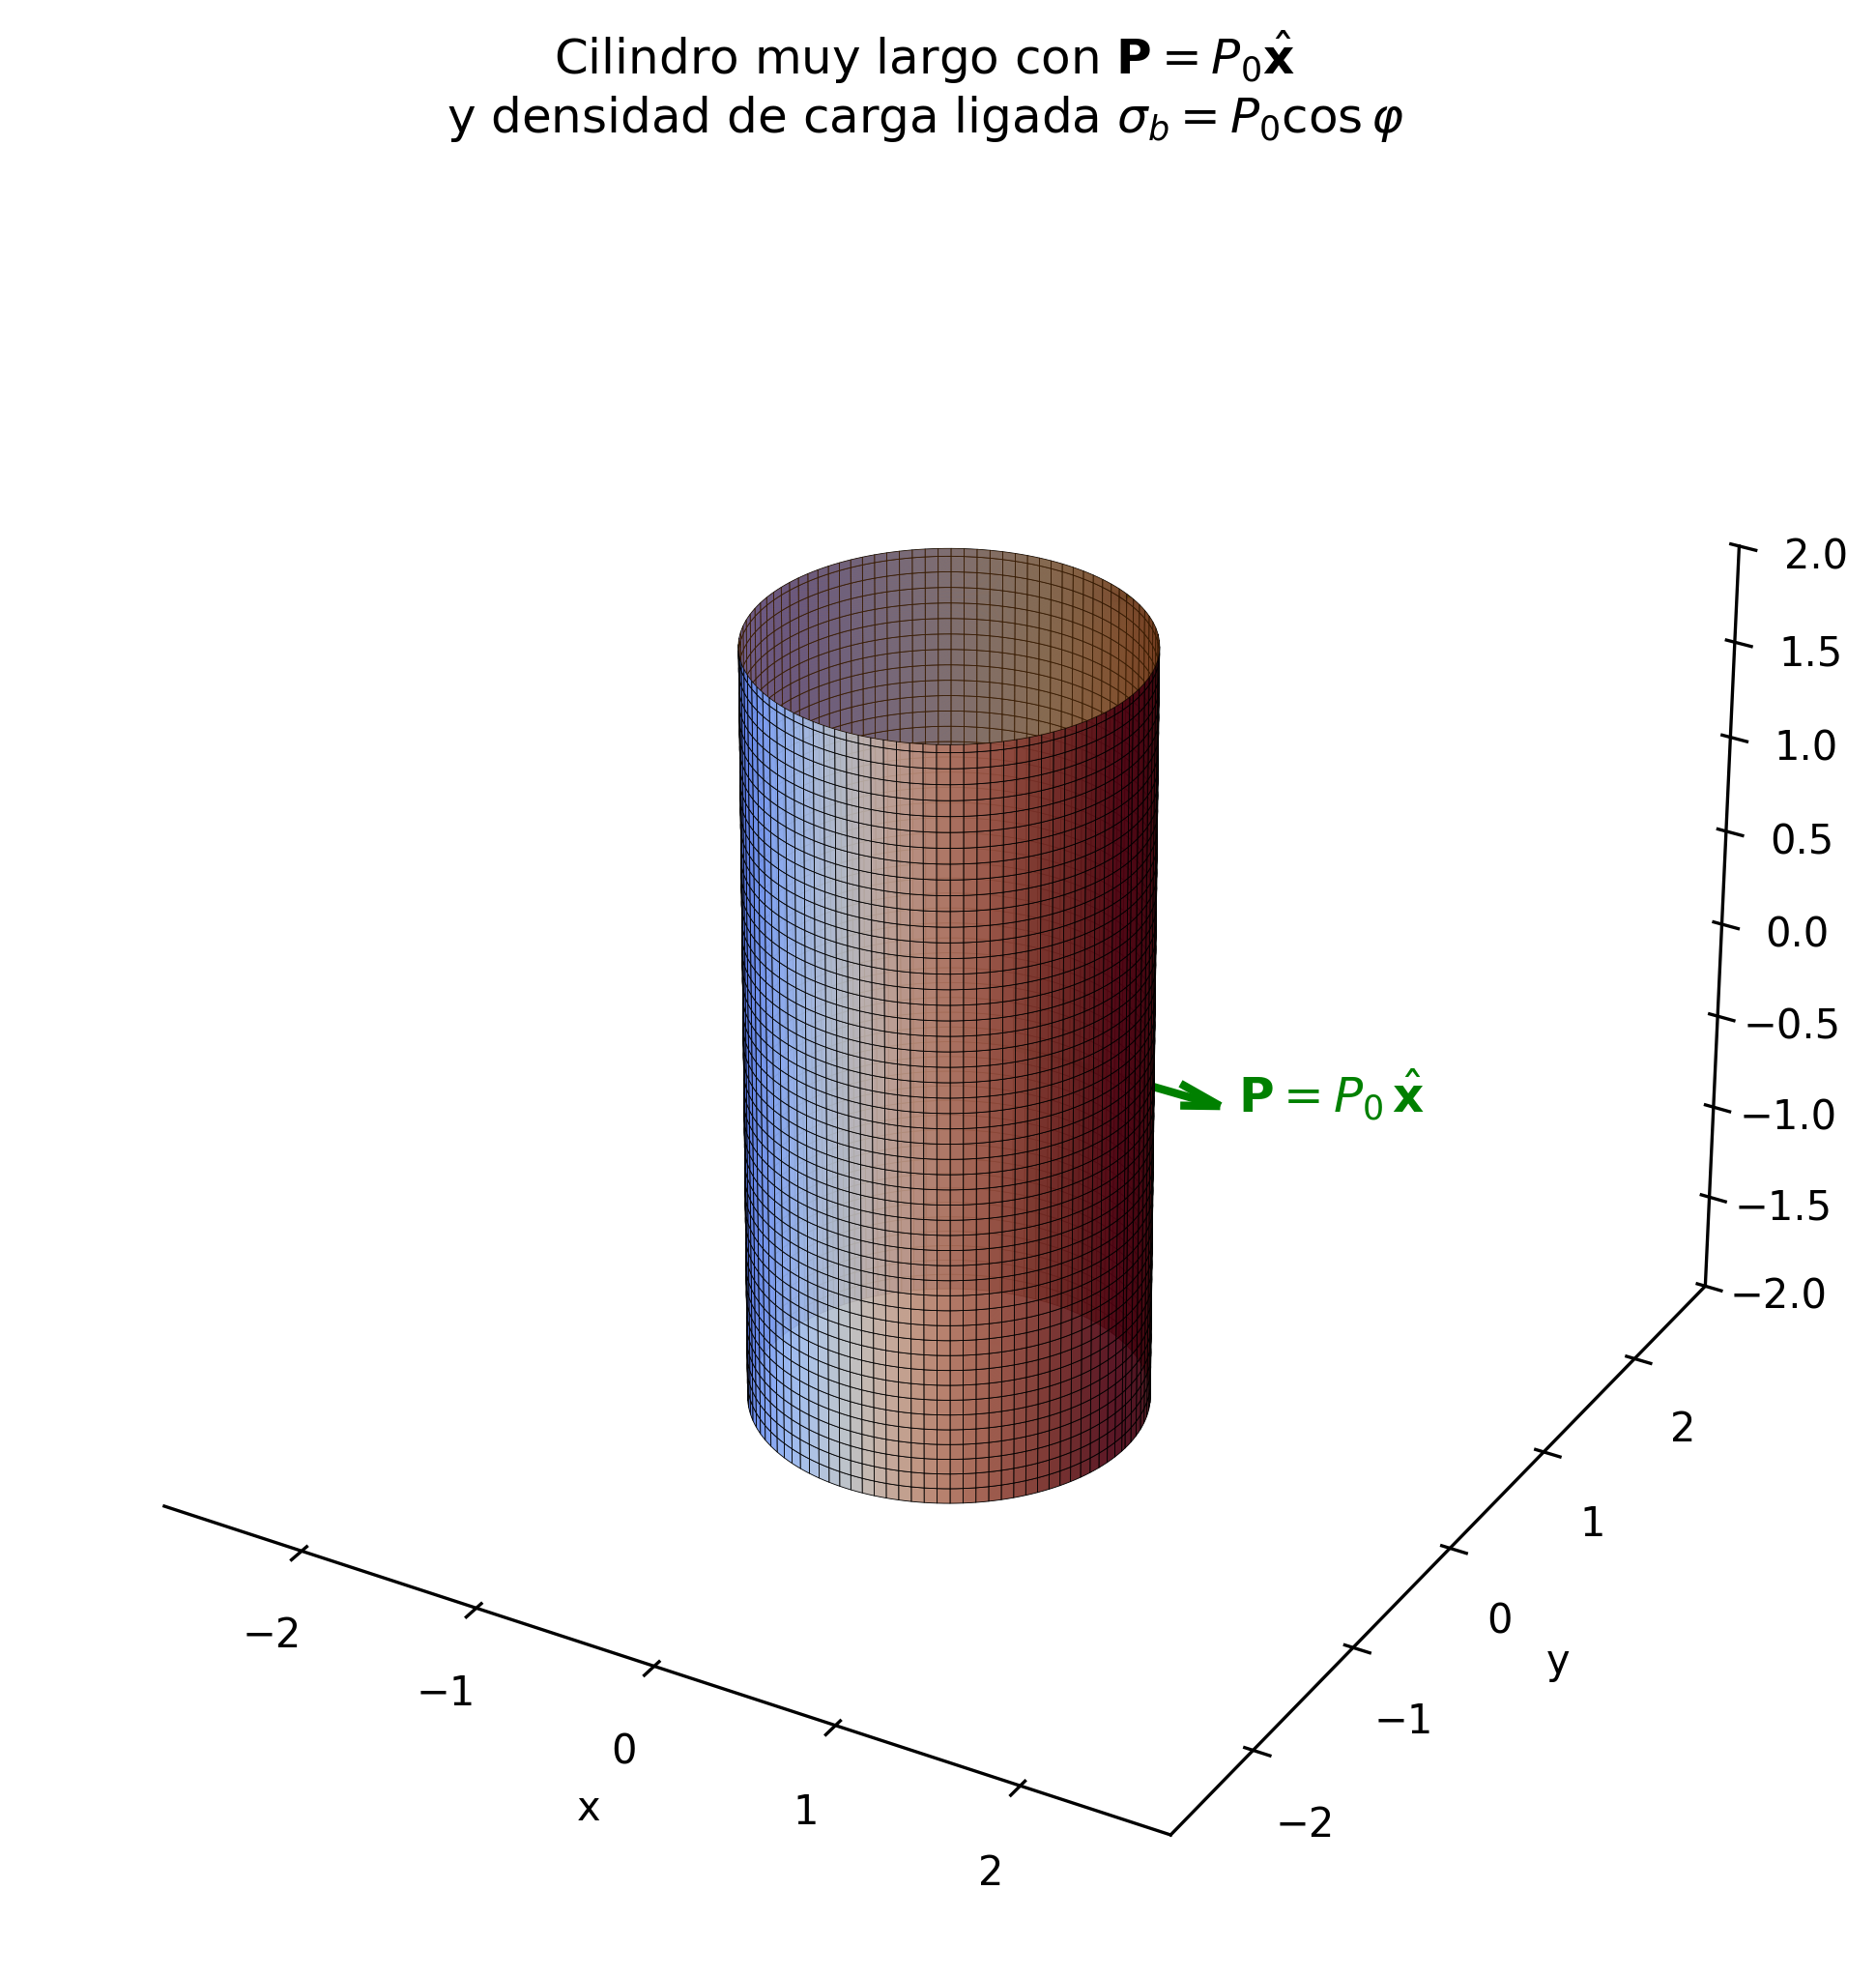
\includegraphics[width=0.70\linewidth]{cilindro_P_perp_sigma.png}

    \vspace{2mm}
    \small
    \textbf{Figura X.} Cilindro muy largo de radio $a$, con polarización uniforme 
    $\mathbf{P} = P_{0}\hat{\mathbf{x}}$ perpendicular al eje. En la superficie 
    lateral se representa la densidad de carga ligada 
    $\sigma_{b} = P_{0}\cos\varphi$, positiva en el lado donde $\mathbf{P}$ 
    apunta hacia afuera del material y negativa en el lado opuesto.
\end{center}

Consideremos un cilindro muy largo (idealmente infinito) de radio $a$ cuyo eje 
coincide con el eje $z$. La polarización es uniforme y está dirigida 
perpendicularmente al eje. Sin pérdida de generalidad podemos elegir
\begin{equation}
\mathbf{P} = P_{0}\,\hat{\mathbf{x}}
\label{eq:P-cilindro-perp}
\end{equation}
donde $P_{0}$ es la magnitud de la polarización. El problema consiste en 
determinar las cargas ligadas y el campo eléctrico que produce esta 
polarización en toda la región espacial.

%====================================================================
\subsubsection*{Cargas ligadas}
%====================================================================

En medios polarizados, las cargas ligadas se obtienen directamente a partir del 
campo de polarización:
\begin{align}
\rho_{b} &= -\,\nabla\cdot\mathbf{P}
\qquad\text{(densidad de carga ligada de volumen)}
\label{eq:rho-b-def-3}\\[4pt]
\sigma_{b} &= \mathbf{P}\cdot\hat{\mathbf{n}}
\qquad\text{(densidad de carga ligada superficial)}
\label{eq:sigma-b-def-3}
\end{align}
Estos resultados provienen del modelo microscópico en el que la materia está 
formada por dipolos eléctricos: si la polarización varía dentro del volumen 
aparece carga ligada de volumen; si el material termina abruptamente, aparece 
carga ligada superficial proporcional a la componente normal de $\mathbf{P}$.

%-----------------------------------------------------
\paragraph{Densidad volumétrica $\rho_{b}$}
%-----------------------------------------------------

La polarización $\mathbf{P}$ es completamente uniforme en todo el volumen, de 
modo que su divergencia es nula:
\begin{equation}
\nabla\cdot\mathbf{P} = 0
\quad\Rightarrow\quad
\rho_{b} = 0
\label{eq:rho-b-3-final}
\end{equation}
No surge carga ligada de volumen porque no hay ningún cambio espacial en la 
orientación o magnitud de los dipolos dentro del material.

%-----------------------------------------------------
\paragraph{Densidad superficial $\sigma_{b}$}
%-----------------------------------------------------

La única superficie del cilindro (al ser infinito en $z$) es la pared lateral. 
En dicha superficie, la normal saliente es puramente radial en el plano 
transversal:
\begin{equation}
\hat{\mathbf{n}} = \hat{\mathbf{s}}
\label{eq:n-hat-cilindro}
\end{equation}
donde $(s,\phi)$ son coordenadas cilíndricas perpendiculares al eje.

Para evaluar $\sigma_{b}$ recordemos que, por definición,
\[
\sigma_{b} = \mathbf{P}\cdot\hat{\mathbf{n}},
\]
y en la pared lateral del cilindro la normal saliente es radial:
\[
\hat{\mathbf{n}} = \hat{\mathbf{s}}.
\]
Así que lo único que necesitamos es el \textbf{producto punto} entre la
polarización $\mathbf{P}$ y el vector radial $\hat{\mathbf{s}}$.

\medskip

Primero, describamos con calma quién es quién en el plano $xy$:

\begin{itemize}
  \item En coordenadas cilíndricas, un punto del plano se escribe como
  \[
  x = s\cos\phi,
  \qquad
  y = s\sin\phi
  \]
  donde $s$ es la distancia al eje $z$ y $\phi$ es el ángulo medido desde el eje $x$.
  
  \item El vector unitario \emph{radial} (apuntando hacia afuera) es
  \[
  \hat{\mathbf{s}} = (\cos\phi)\,\hat{\mathbf{x}} + (\sin\phi)\,\hat{\mathbf{y}}.
  \]
  
  \item El vector unitario \emph{tangencial} (girando en sentido antihorario) es
  \[
  \hat{\boldsymbol{\phi}} = (-\sin\phi)\,\hat{\mathbf{x}} + (\cos\phi)\,\hat{\mathbf{y}}.
  \]
\end{itemize}

Estas dos expresiones forman una especie de “cambio de base’’ entre
$(\hat{\mathbf{x}},\hat{\mathbf{y}})$ y $(\hat{\mathbf{s}},\hat{\boldsymbol{\phi}})$.
Si las invertimos, obtenemos (puede verificarse haciendo la combinación lineal):
\begin{equation}
\hat{\mathbf{x}} = \cos\phi\,\hat{\mathbf{s}} - \sin\phi\,\hat{\boldsymbol{\phi}},
\qquad
\hat{\mathbf{y}} = \sin\phi\,\hat{\mathbf{s}} + \cos\phi\,\hat{\boldsymbol{\phi}}.
\label{eq:x-y-en-cilindricas-detallado}
\end{equation}

Ahora volvamos a la polarización. El problema nos dice que
\[
\mathbf{P} = P_{0}\,\hat{\mathbf{x}}.
\]
Usando \eqref{eq:x-y-en-cilindricas-detallado} para $\hat{\mathbf{x}}$,
podemos escribir $\mathbf{P}$ en la base cilíndrica:
\begin{equation}
\mathbf{P}
= P_{0}\,\hat{\mathbf{x}}
= P_{0}\bigl(\cos\phi\,\hat{\mathbf{s}} - \sin\phi\,\hat{\boldsymbol{\phi}}\bigr).
\label{eq:P-en-cilindricas-detallado}
\end{equation}

Con esto ya tenemos listos los ingredientes para la carga superficial ligada.
En la superficie lateral ($s=a$) la normal es $\hat{\mathbf{n}}=\hat{\mathbf{s}}$, así que
\begin{align}
\sigma_{b}
&= \mathbf{P}\cdot\hat{\mathbf{n}}
= \mathbf{P}\cdot\hat{\mathbf{s}}
\label{eq:sigma-paso1}\\[4pt]
&= P_{0}\bigl(\cos\phi\,\hat{\mathbf{s}} - \sin\phi\,\hat{\boldsymbol{\phi}}\bigr)\cdot\hat{\mathbf{s}}
\label{eq:sigma-paso2}\\[4pt]
&= P_{0}\bigl(\cos\phi\,\underbrace{\hat{\mathbf{s}}\cdot\hat{\mathbf{s}}}_{=1}
               - \sin\phi\,\underbrace{\hat{\boldsymbol{\phi}}\cdot\hat{\mathbf{s}}}_{=0}\bigr)
\label{eq:sigma-paso3}\\[4pt]
&= P_{0}\cos\phi.
\label{eq:sigma-b-3-final-detallado}
\end{align}

En palabras sencillas:
\begin{itemize}
  \item Sólo importa la componente de $\mathbf{P}$ en la dirección de la normal
  $\hat{\mathbf{s}}$.
  \item Esa componente vale $P_{0}\cos\phi$ (porque $\mathbf{P}$ apunta fijo en $+x$,
  y la normal forma un ángulo $\phi$ con ese eje).
  \item Por eso la carga ligada superficial es máxima y positiva en el lado
  $\phi=0$ (eje $+x$), máxima y negativa en $\phi=\pi$ (eje $-x$) y nula en
  los puntos laterales $\phi=\pi/2$ y $3\pi/2$.
\end{itemize}


Así, la carga superficial ligada varía como $\cos\phi$: es positiva en el lado 
del cilindro orientado hacia $+x$ y negativa en el lado orientado hacia $-x$. 
No hay carga en los “extremos’’ porque el cilindro es infinitamente largo.

%====================================================================
\subsubsection*{Potencial electrostático (explicado como para un bebé)}
%====================================================================

Primero recordemos una idea muy simple: el potencial eléctrico $V$ es como una 
“altura” que genera el campo eléctrico, y las cargas en la superficie del 
cilindro hacen que esta “altura” cambie alrededor del cilindro.

El cilindro es muy, muy largo (casi infinito), así que todo es igual en la 
dirección $z$. Eso significa que el problema solo depende de 
dónde estés en el \emph{plano} $(x,y)$, o sea, es un problema de dos 
dimensiones. Por eso el potencial debe satisfacer:
\[
\nabla^{2}V = 0,
\]
que es la ecuación de Laplace: la ecuación que vale cuando no hay cargas 
\emph{dentro} sino solo en la superficie.

Ahora, ¿cómo sabemos la forma del potencial?  
La carga superficial cambia como $\cos\phi$: eso significa que el lado del 
cilindro hacia $+x$ está “más cargado” y el lado hacia $-x$ está “menos 
cargado”, siguiendo una variación suave alrededor del círculo.  
Cuando una cosa cambia como $\cos\phi$, la solución del potencial también tiene
que tener esa misma forma angular. Es como una huella digital: si la carga tiene
$\cos\phi$, la solución también.

Por eso la forma más simple posible para el potencial es:

\[
V(s,\phi)
=
\begin{cases}
A\,s\cos\phi, & s<a,\\[4pt]
B\,\dfrac{a^{2}}{s}\cos\phi, & s>a.
\end{cases}
\]

¿Por qué esas formas?

- \textbf{Dentro ($s<a$):} usamos $A\,s\cos\phi$ porque:
  - es proporcional a $s$ (no explota en el centro),
  - tiene la misma forma angular $\cos\phi$ que la carga en la superficie.

- \textbf{Fuera ($s>a$):} usamos $B\,a^{2}\cos\phi/s$ porque:
  - decrece cuando te alejas del cilindro (como debe hacerlo una fuente finita),
  - también tiene $\cos\phi$,
  - la forma $1/s$ es la solución “suave” de Laplace en 2D que se va a cero.

Hasta aquí no hemos usado ninguna condición física concreta: sólo dijimos
“escojo las formas más simples que respeten las reglas básicas”.

%-----------------------------------------------------
\paragraph{Condiciones de frontera (como para un bebé)}
%-----------------------------------------------------

Ahora tenemos que encontrar $A$ y $B$. Para eso usamos dos reglas que siempre 
valen en electrostática:

\begin{enumerate}
  \item \textbf{El potencial no puede tener saltos}.  
  Es como una superficie continua: si hubiera un salto, sería como un escalón 
  infinito sin razón. Por eso en $s=a$ debe cumplirse:
  \[
  A a\cos\phi = B a\cos\phi
  \quad\Rightarrow\quad
  A = B.
  \]

  \item \textbf{El campo normal sí puede tener un salto}, y ese salto está
  completamente dictado por la carga superficial.  
  Esta es una regla universal:  
  \[
  \epsilon_{0}(E_{s}^{\text{out}} - E_{s}^{\text{in}}) = \sigma_{b}(\phi).
  \]
  Y ya sabemos que la carga superficial es:
  \[
  \sigma_{b}(\phi) = P_{0}\cos\phi.
  \]

  Ahora necesitamos las derivadas:
  \[
  E_{s}^{\text{in}} = -A\cos\phi,
  \qquad
  E_{s}^{\text{out}} = B\cos\phi.
  \]

  Metiéndolo en la ecuación del salto:
  \[
  \epsilon_{0}(B\cos\phi - (-A\cos\phi)) = P_{0}\cos\phi.
  \]

  Como ya sabemos que $A = B$:
  \[
  \epsilon_{0}(A + A)\cos\phi = P_{0}\cos\phi
  \]
  lo cual nos da directamente:
  \[
  2\epsilon_{0}A = P_{0}
  \quad\Rightarrow\quad
  A = B = \frac{P_{0}}{2\epsilon_{0}}.
  \]
\end{enumerate}

¡Listo! Ya encontramos los dos números mágicos.

%====================================================================
\subsubsection*{Campo eléctrico dentro y fuera (como para un bebé)}
%====================================================================

%-------------------------
\paragraph{Interior ($s<a$)}
%-------------------------

El potencial interior es simplemente:
\[
V_{\text{in}}(s,\phi)
= \frac{P_{0}}{2\epsilon_{0}}\,s\cos\phi.
\]

Pero recuerda que:
\[
s\cos\phi = x,
\]
así que:
\[
V_{\text{in}}(x,y)
= \frac{P_{0}}{2\epsilon_{0}}\,x.
\]

Si el potencial es como una inclinación, entonces el campo eléctrico es la
pendiente de esa inclinación, pero hacia abajo:
\[
\mathbf{E}_{\text{in}} = -\nabla V_{\text{in}}.
\]

Derivando:
\[
\mathbf{E}_{\text{in}}
= -\frac{P_{0}}{2\epsilon_{0}}\hat{\mathbf{x}}
= -\,\frac{\mathbf{P}}{2\epsilon_{0}}.
\]

\textbf{Interpretación bebé:}  
El cilindro, por dentro, tiene un campo uniforme que apunta exactamente en la
dirección contraria a la polarización. Como si la materia “se resistiera” a la
orientación impuesta.

%-------------------------
\paragraph{Exterior ($s>a$)}
%-------------------------

El potencial exterior es:
\[
V_{\text{out}}(s,\phi)
= \frac{P_{0}}{2\epsilon_{0}}\frac{a^{2}}{s}\cos\phi.
\]

Derivando lentamente obtenemos las dos componentes del campo:
\[
E_{s}
= \frac{P_{0}a^{2}}{2\epsilon_{0}s^{2}}\cos\phi,
\qquad
E_{\phi}
= \frac{P_{0}a^{2}}{2\epsilon_{0}s^{2}}\sin\phi.
\]

El campo total es la suma de ambas:
\[
\mathbf{E}_{\text{out}}
= \frac{P_{0}a^{2}}{2\epsilon_{0}s^{2}}
   \bigl(\cos\phi\,\hat{\mathbf{s}}
        + \sin\phi\,\hat{\boldsymbol{\phi}}\bigr).
\]

Esto se puede reescribir de una forma mucho más elegante usando vectores:
\[
\boxed{
\mathbf{E}_{\text{out}}(s)
= \frac{a^{2}}{2\epsilon_{0}s^{2}}
  \bigl[\,2(\mathbf{P}\cdot\hat{\mathbf{s}})\hat{\mathbf{s}}
        - \mathbf{P}\,\bigr]
}
\qquad (s>a).
\]

%====================================================================
\subsubsection*{Resumen (como una colección de cromos)}
%====================================================================

\begin{align}
\rho_{b} &= 0 
\qquad\text{(no hay carga ligada en el volumen)},\\[4pt]
\sigma_{b}(\phi) &= P_{0}\cos\phi 
\qquad\text{(más carga en el lado que apunta $\mathbf{P}$)},\\[4pt]
\mathbf{E}_{\text{in}} &= -\,\dfrac{\mathbf{P}}{2\epsilon_{0}}
\qquad\text{(campo constante hacia el lado opuesto)},\\[4pt]
\mathbf{E}_{\text{out}}(s)
&= \dfrac{a^{2}}{2\epsilon_{0}s^{2}}
   \bigl[\,2(\mathbf{P}\cdot\hat{\mathbf{s}})\hat{\mathbf{s}}
        - \mathbf{P}\,\bigr]
\qquad\text{(campo tipo dipolar alrededor)}.
\end{align}



\section{Problema 4}

\textcolor{Cinnabar}{\textbf{Solución Pr. 4.4}} \vspace{0.4cm}

Tenemos una \textbf{cáscara esférica gruesa} (como una cebolla esférica) con:

- radio interno $a$ (empieza el material),  
- radio externo $b$ (termina el material).

Entre $a$ y $b$ hay material dieléctrico; para $r<a$ hay un hueco, y para
$r>b$ ya no hay dieléctrico.  
La polarización es \textbf{radial} y está “congelada’’ (no cambia con el
tiempo):

\begin{equation}
\mathbf{P}(r) = \frac{k}{r}\,\hat{\mathbf{r}},
\label{eq:P-shell}
\end{equation}

donde $k$ es una constante y $r$ la distancia al centro de la esfera.  
La polarización sólo vive en la región

\[
a<r<b.
\]

No hay carga libre, así que TODO el campo eléctrico se debe a \textbf{cargas
ligadas}.

%====================================================================
\subsubsection*{1. Cargas ligadas $\rho_{b}$ y $\sigma_{b}$}
%====================================================================

En un dieléctrico polarizado sabemos que:

\begin{align}
\rho_{b} &= - \nabla\cdot\mathbf{P}
\label{eq:rho-b-def-shell} \\
\sigma_{b} &= \mathbf{P}\cdot\hat{\mathbf{n}},
\label{eq:sigma-b-def-shell}
\end{align}

donde:

- $\rho_{b}$ es la \textbf{densidad de carga ligada de volumen}
  (carga “pegada” dentro del material),
- $\sigma_{b}$ es la \textbf{densidad de carga ligada superficial}
  (carga “pegada” en la superficie),
- $\hat{\mathbf{n}}$ es la normal \emph{saliente del material}
  (muy importante para el signo).

%----------------------------------------------------
\paragraph{(a) Carga ligada de volumen $\rho_{b}$}
%----------------------------------------------------

Como la polarización es radial, usamos la fórmula para la divergencia de un
campo del tipo

\[
\mathbf{A}(r) = f(r)\,\hat{\mathbf{r}}.
\]

En coordenadas esféricas, la divergencia es

\begin{equation}
\nabla\cdot\mathbf{A} = \frac{1}{r^{2}}\,\frac{d}{dr}\bigl(r^{2} f(r)\bigr).
\label{eq:div-radial}
\end{equation}

En nuestro problema, la función radial es

\[
f(r)=\frac{k}{r},
\]

así que primero calculamos

\begin{equation}
r^{2}f(r) = r^{2}\,\frac{k}{r} = k\,r.
\label{eq:r2f}
\end{equation}

Luego derivamos:

\[
\frac{d}{dr}(kr) = k.
\]

Metiendo esto en \eqref{eq:div-radial}:

\begin{equation}
\nabla\cdot\mathbf{P}
= \frac{1}{r^{2}}\frac{d}{dr}(kr)
= \frac{k}{r^{2}}.
\label{eq:div-P-shell}
\end{equation}

Como $\rho_{b}=-\nabla\cdot\mathbf{P}$, resulta

\begin{equation}
\rho_{b} = -\nabla\cdot\mathbf{P}
= -\frac{k}{r^{2}}
\qquad\text{para } a<r<b.
\label{eq:rho-b-shell}
\end{equation}

Fuera del material, la polarización es cero:
$\mathbf{P}=\mathbf{0}$ para $r<a$ y $r>b$, así que también lo es la
densidad de carga ligada de volumen:

\begin{equation}
\rho_{b} = 0 \quad \text{para } r<a \text{ y } r>b.
\label{eq:rho-b-cero-fuera}
\end{equation}

%----------------------------------------------------
\paragraph{(b) Carga ligada superficial $\sigma_{b}$}
%----------------------------------------------------

El material termina en dos superficies:

- la cara interna en $r=a$,  
- la cara externa en $r=b$.

En cada una usamos:

\[
\sigma_{b} = \mathbf{P}\cdot\hat{\mathbf{n}},
\]

donde $\hat{\mathbf{n}}$ es el vector normal que \emph{sale del dieléctrico}
(no necesariamente hacia afuera del espacio, sino \emph{fuera del material}).

\medskip

\textbf{Superficie externa ($r=b$).}  

En el borde exterior el dieléctrico termina y lo que sigue es el vacío hacia
afuera, por lo que la normal saliente del material apunta radialmente hacia
afuera:

\begin{equation}
\hat{\mathbf{n}}_{\text{ext}} = \hat{\mathbf{r}}.
\label{eq:n-ext}
\end{equation}

En $r=b$ la polarización vale

\begin{equation}
\mathbf{P}(b) = \frac{k}{b}\,\hat{\mathbf{r}}.
\label{eq:P-b}
\end{equation}

Entonces la densidad superficial es

\begin{equation}
\sigma_{b}^{(\text{ext})}
= \mathbf{P}(b)\cdot\hat{\mathbf{n}}_{\text{ext}}
= \frac{k}{b}\,\hat{\mathbf{r}}\cdot\hat{\mathbf{r}}
= \frac{k}{b}.
\label{eq:sigma-ext}
\end{equation}

Es una carga ligada \textbf{positiva} repartida sobre toda la esfera de radio
$b$.

\medskip

\textbf{Superficie interna ($r=a$).}  

Aquí el material está “pegado” al hueco interior.  
La normal saliente del dieléctrico apunta hacia el hueco, es decir, hacia
adentro en sentido radial:

\begin{equation}
\hat{\mathbf{n}}_{\text{int}} = -\hat{\mathbf{r}}.
\label{eq:n-int}
\end{equation}

En $r=a$ la polarización vale

\begin{equation}
\mathbf{P}(a) = \frac{k}{a}\,\hat{\mathbf{r}}.
\label{eq:P-a}
\end{equation}

Por tanto,

\begin{equation}
\sigma_{b}^{(\text{int})}
= \mathbf{P}(a)\cdot\hat{\mathbf{n}}_{\text{int}}
= \frac{k}{a}\,\hat{\mathbf{r}}\cdot(-\hat{\mathbf{r}})
= -\frac{k}{a}.
\label{eq:sigma-int}
\end{equation}

Es una carga ligada \textbf{negativa} en la superficie esférica de radio $a$.

\medskip

\textbf{Resumen de cargas ligadas:}

\begin{align}
\rho_{b}(r) &= -\dfrac{k}{r^{2}} \quad \text{para } a<r<b,
\qquad \rho_{b}=0 \text{ fuera},
\\[4pt]
\sigma_{b}(r=a) &= -\dfrac{k}{a},
\\[4pt]
\sigma_{b}(r=b) &= +\dfrac{k}{b}.
\end{align}

%====================================================================
\subsubsection*{2. Verificación de neutralidad total}
%====================================================================

Ahora comprobamos que, sumando todas las cargas ligadas (volumen + superficies),
el total es cero.

\paragraph{Carga ligada de volumen.}

Usamos

\[
Q_{b}^{(\text{vol})} = \int_{V} \rho_{b}\,d\tau,
\]

donde $d\tau$ es el elemento de volumen. En coordenadas esféricas  
$d\tau = r^{2}\sin\theta\,dr\,d\theta\,d\phi$, pero como $\rho_{b}$ sólo depende
de $r$, la integral angular nos da $4\pi$ y podemos escribir:

\begin{equation}
Q_{b}^{(\text{vol})}
= \int_{a}^{b}\left(-\frac{k}{r^{2}}\right)4\pi r^{2}\,dr
= -4\pi k\int_{a}^{b}dr
= -4\pi k(b-a).
\label{eq:Qb-vol-shell}
\end{equation}

\paragraph{Cargas ligadas superficiales.}

En una esfera de radio $R$, el área total es $4\pi R^{2}$, así que
$\int_{S}da = 4\pi R^{2}$.

\medskip

\textbf{Superficie externa ($r=b$):}

\begin{equation}
Q_{b}^{(\text{ext})}
= \int_{S_{b}} \sigma_{b}^{(\text{ext})}\,da
= \left(\frac{k}{b}\right)(4\pi b^{2})
= 4\pi k b.
\label{eq:Qb-ext}
\end{equation}

\textbf{Superficie interna ($r=a$):}

\begin{equation}
Q_{b}^{(\text{int})}
= \int_{S_{a}} \sigma_{b}^{(\text{int})}\,da
= \left(-\frac{k}{a}\right)(4\pi a^{2})
= -4\pi k a.
\label{eq:Qb-int}
\end{equation}

\paragraph{Suma total.}

Sumando:

\begin{equation}
Q_{b}^{\text{(total)}}
= Q_{b}^{(\text{vol})} + Q_{b}^{(\text{ext})} + Q_{b}^{(\text{int})}
= \bigl(-4\pi k(b-a)\bigr) + 4\pi k b - 4\pi k a = 0.
\label{eq:Qb-total-shell}
\end{equation}

La cáscara completa es \textbf{globalmente neutra}: tiene cargas ligadas, pero
la suma total es cero.

%====================================================================
\subsubsection*{3. Campo eléctrico mediante la ley de Gauss}
%====================================================================

Por simetría esférica, el campo eléctrico sólo puede ser radial y depender de
$r$:

\begin{equation}
\mathbf{E}(\mathbf{r}) = E(r)\,\hat{\mathbf{r}}.
\label{eq:E-r-shell}
\end{equation}

Usamos la ley de Gauss en forma integral:

\begin{equation}
\oint_{S} \mathbf{E}\cdot d\mathbf{a}
= \frac{1}{\epsilon_{0}}\,Q_{\text{enc}}(r),
\label{eq:gauss-shell}
\end{equation}

donde $Q_{\text{enc}}(r)$ es la carga ligada encerrada por una superficie
gaussiana esférica de radio $r$.

En una esfera, $d\mathbf{a} = \hat{\mathbf{r}}\,r^{2}\sin\theta\,d\theta\,d\phi$
y, como $\mathbf{E} = E(r)\hat{\mathbf{r}}$, el flujo es siempre:

\[
\oint_{S} \mathbf{E}\cdot d\mathbf{a} = E(r)\,(4\pi r^{2}).
\]

Ahora analizamos tres regiones.

%----------------------------------------------------
\paragraph{(i) Región $r<a$ (hueco interno)}
%----------------------------------------------------

La superficie gaussiana está completamente dentro del hueco, donde no hay
material ni cargas ligadas:

\begin{equation}
Q_{\text{enc}}(r<a) = 0.
\label{eq:Qenc-inner}
\end{equation}

Entonces la ley de Gauss nos da:

\[
E(r)\,(4\pi r^{2}) = 0
\quad\Rightarrow\quad
E(r)=0.
\]

Por lo tanto,

\begin{equation}
\mathbf{E}(\mathbf{r}) = \mathbf{0}
\qquad \text{para } r<a.
\label{eq:E-inner-final}
\end{equation}

%----------------------------------------------------
\paragraph{(ii) Región $a<r<b$ (dentro del dieléctrico)}
%----------------------------------------------------

Ahora la esfera gaussiana:

- sí encierra la superficie interna ($r=a$),  
- y encierra la carga de volumen desde $r=a$ hasta $r=r$,  
- pero \emph{todavía no} encierra la superficie externa ($r=b$).

\medskip

\textbf{Carga de volumen entre $a$ y $r$:}

\begin{equation}
Q_{\text{vol}}(a\to r)
= \int_{a}^{r} \left(-\frac{k}{r'^{2}}\right)4\pi r'^{2}\,dr'
= -4\pi k\int_{a}^{r}dr'
= -4\pi k(r-a).
\label{eq:Qvol-a-r}
\end{equation}

\textbf{Carga superficial interna:} ya la conocemos:

\begin{equation}
Q_{b}^{(\text{int})} = -4\pi k a.
\label{eq:Q-int-record}
\end{equation}

\textbf{Carga total encerrada:}

\begin{equation}
Q_{\text{enc}}(r)
= Q_{b}^{(\text{int})} + Q_{\text{vol}}(a\to r)
= \bigl(-4\pi k a\bigr) + \bigl(-4\pi k(r-a)\bigr)
= -4\pi k r.
\label{eq:Qenc-a-r-b}
\end{equation}

El flujo es

\begin{equation}
\oint_{S} \mathbf{E}\cdot d\mathbf{a}
= E(r)\,(4\pi r^{2}).
\label{eq:flujo-a-r-b}
\end{equation}

Aplicando Gauss:

\begin{equation}
E(r)\,(4\pi r^{2})
= \frac{1}{\epsilon_{0}}\bigl(-4\pi k r\bigr),
\label{eq:gauss-a-r-b}
\end{equation}

de donde:

\begin{equation}
E(r) = -\,\frac{k}{\epsilon_{0}}\,\frac{1}{r}.
\label{eq:E-magn-a-r-b}
\end{equation}

Esto significa que:

\begin{equation}
\boxed{
\mathbf{E}(\mathbf{r})
= -\,\frac{k}{\epsilon_{0}}\,\frac{1}{r}\,\hat{\mathbf{r}},
\qquad a<r<b.
}
\label{eq:E-vector-a-r-b}
\end{equation}

El campo apunta radialmente hacia el centro si $k>0$ (es decir, dirección
$-\hat{\mathbf{r}}$).

%----------------------------------------------------
\paragraph{(iii) Región $r>b$ (exterior)}
%----------------------------------------------------

Para $r>b$, la esfera gaussiana encierra:

- toda la carga de volumen entre $a$ y $b$,  
- más ambas superficies ($r=a$ y $r=b$).

Pero en la sección anterior ya demostramos que la carga total ligada es cero:

\[
Q_{\text{enc}}(r>b) = Q_{b}^{\text{(total)}} = 0.
\]

Entonces, otra vez, por Gauss:

\[
E(r)\,(4\pi r^{2}) = 0
\quad\Rightarrow\quad
\mathbf{E}(\mathbf{r}) = \mathbf{0}
\qquad\text{para } r>b.
\]

\begin{equation}
\label{eq:E-outer-final}
\end{equation}

%====================================================================
\subsubsection*{Resumen final}
%====================================================================

\textbf{Cargas ligadas:}
\begin{align}
\rho_{b}(r) &= -\dfrac{k}{r^{2}} \quad \text{para } a<r<b,
\qquad \rho_{b}=0 \text{ fuera},\\[4pt]
\sigma_{b}(r=a) &= -\dfrac{k}{a},\\[4pt]
\sigma_{b}(r=b) &= +\dfrac{k}{b}.
\end{align}

\textbf{Campo eléctrico total:}
\begin{equation}
\mathbf{E}(\mathbf{r}) =
\begin{cases}
\mathbf{0}, & r<a,\\[4pt]
-\dfrac{k}{\epsilon_{0}}\dfrac{1}{r}\,\hat{\mathbf{r}}, & a<r<b,\\[6pt]
\mathbf{0}, & r>b.
\end{cases}
\label{eq:E-piecewise-shell}
\end{equation}


\section{Problema 5 (versión “para bebé nerd de física”)}

\textcolor{Cinnabar}{\textbf{Solución Pr. 5.5}} \vspace{0.4cm}

En este problema estudiamos un \textbf{capacitor de placas paralelas} de área $A$ y separación $d$.  
Cuando entre las placas hay solo \textbf{vacío} (o aire, que es casi lo mismo para estos fines), su capacitancia es

\begin{equation}
C_{0} = \frac{\epsilon_{0}A}{d}
\label{eq:C0-capacitor}
\end{equation}

donde:
\begin{itemize}
  \item $\epsilon_{0}$ es la \textbf{permitividad del vacío}
  \item $A$ es el \textbf{área} de cada placa
  \item $d$ es la \textbf{distancia} entre placas
\end{itemize}

Esta fórmula se puede recordar así: para un capacitor plano con placas grandes y separación pequeña, el campo es aproximadamente uniforme, $E = V/d$, y la densidad de carga libre es $\sigma_{f} = \epsilon_{0}E$. Como $Q = \sigma_{f}A$ y $V = Ed$, entonces

\[
C = \frac{Q}{V} = \frac{\epsilon_{0}EA}{Ed} = \frac{\epsilon_{0}A}{d}
\]

Ahora introducimos un \textbf{dieléctrico} de constante dieléctrica relativa $\epsilon_{r}$, pero solo “llenamos a la mitad’’ el capacitor de dos formas diferentes:

\begin{itemize}
  \item[(a)] Bloque dieléctrico que ocupa \textbf{todo el área $A$} pero solo \textbf{la mitad de la separación} ($d/2$)
  \item[(b)] Bloque dieléctrico que ocupa \textbf{la mitad del área} ($A/2$) pero \textbf{toda la separación} $d$
\end{itemize}

Se pide:
\begin{enumerate}
  \item Encontrar por qué \textbf{fracción} se incrementa la capacitancia en cada caso, es decir, calcular $C_{\text{eq}}/C_{0}$ y el incremento relativo
  \item Para un potencial fijo $V$ entre placas, encontrar los campos $\mathbf{E}$, $\mathbf{D}$, la polarización $\mathbf{P}$ en cada región, y las cargas libres y ligadas
\end{enumerate}

Antes de separar casos, recordemos:
\begin{itemize}
  \item $\mathbf{E}$ es el \textbf{campo eléctrico}
  \item $\mathbf{D}$ es el \textbf{desplazamiento eléctrico} y se relaciona con $\mathbf{E}$ y $\mathbf{P}$ mediante
    \[
      \mathbf{D} = \epsilon_{0}\mathbf{E} + \mathbf{P}
    \]
  \item En un \textbf{medio lineal e isotrópico}, también se suele escribir
    \[
      \mathbf{D} = \epsilon \mathbf{E}
      \quad\text{con}\quad
      \epsilon = \epsilon_{r}\epsilon_{0}
    \]
  \item $\mathbf{P}$ es la \textbf{polarización}, que representa el \textbf{dipolo eléctrico por unidad de volumen}
  \item La \textbf{susceptibilidad eléctrica} $\chi_{e}$ se relaciona con $\epsilon_{r}$ por
    \[
      \epsilon_{r} = 1 + \chi_{e}
    \]
    y
    \[
      \mathbf{P} = \epsilon_{0}\chi_{e}\mathbf{E}
      = \epsilon_{0}(\epsilon_{r} - 1)\mathbf{E}
    \]
  \item La \textbf{carga ligada de volumen} es
    \[
      \rho_{b} = -\nabla\cdot\mathbf{P}
    \]
  \item La \textbf{carga ligada superficial} en una interfaz con normal saliente $\hat{\mathbf{n}}$ es
    \[
      \sigma_{b} = \mathbf{P}\cdot\hat{\mathbf{n}}
    \]
\end{itemize}

%=====================================================
\subsection*{Caso (a): Dieléctrico ocupando la mitad de la separación}
%=====================================================

En este caso, el espacio entre las placas se divide en dos “bloques” apilados en la dirección de la separación:

\begin{itemize}
  \item \textbf{Región I (dieléctrico)}: espesor $d_{1} = d/2$, permitividad $\epsilon_{1} = \epsilon_{r}\epsilon_{0}$
  \item \textbf{Región II (vacío)}: espesor $d_{2} = d/2$, permitividad $\epsilon_{2} = \epsilon_{0}$
\end{itemize}

Geométricamente: placa positiva, luego bloque dieléctrico, luego bloque de vacío, luego placa negativa.  
Eso corresponde a \textbf{dos capacitores en serie}, porque la misma carga pasa “a través” de ambos y las caídas de potencial se suman.

%-----------------------------------------------------
\subsubsection*{(a1) Capacitancia equivalente (modo serie)}
%-----------------------------------------------------

Primero, tratamos cada región como un capacitor plano individual.

\paragraph{Capacitor 1 (dieléctrico):}

Usamos la fórmula general $C = \epsilon A / d$ pero con espesor $d/2$ y $\epsilon = \epsilon_{r}\epsilon_{0}$:

\begin{equation}
C_{1} = \frac{\epsilon_{r}\epsilon_{0}A}{d/2}
\label{eq:C1-a-raw}
\end{equation}

Ahora simplificamos el denominador:

\[
\frac{1}{d/2} = \frac{2}{d}
\]

Entonces

\begin{equation}
C_{1} 
= \epsilon_{r}\epsilon_{0}A\left(\frac{2}{d}\right)
= \frac{2\epsilon_{r}\epsilon_{0}A}{d}
\label{eq:C1-a}
\end{equation}

\paragraph{Capacitor 2 (vacío):}

Aquí la permitividad es $\epsilon_{0}$ y el espesor también es $d/2$:

\begin{equation}
C_{2} = \frac{\epsilon_{0}A}{d/2}
\label{eq:C2-a-raw}
\end{equation}

Análogamente:

\begin{equation}
C_{2} 
= \epsilon_{0}A\left(\frac{2}{d}\right)
= \frac{2\epsilon_{0}A}{d}
\label{eq:C2-a}
\end{equation}

\paragraph{Capacitores en serie:}

Para capacitores en serie, la regla es

\begin{equation}
\frac{1}{C_{\text{eq}}^{(a)}} = \frac{1}{C_{1}} + \frac{1}{C_{2}}
\label{eq:serie-regla}
\end{equation}

La idea física es:
\begin{itemize}
  \item La \textbf{misma carga} $Q$ pasa por todos los capacitores de la serie
  \item El \textbf{voltaje total} es la suma de los voltajes de cada uno
  \item Como $V = Q/C$, se obtiene la combinación en términos de inversos
\end{itemize}

Sustituimos $C_{1}$ y $C_{2}$:

\begin{equation}
\frac{1}{C_{\text{eq}}^{(a)}} 
= \frac{1}{\frac{2\epsilon_{r}\epsilon_{0}A}{d}}
 + \frac{1}{\frac{2\epsilon_{0}A}{d}}
\label{eq:1Ceq-a-paso1}
\end{equation}

Invertimos cada fracción:

\[
\frac{1}{\frac{2\epsilon_{r}\epsilon_{0}A}{d}} = \frac{d}{2\epsilon_{r}\epsilon_{0}A},
\qquad
\frac{1}{\frac{2\epsilon_{0}A}{d}} = \frac{d}{2\epsilon_{0}A}
\]

Entonces

\begin{equation}
\frac{1}{C_{\text{eq}}^{(a)}} 
= \frac{d}{2\epsilon_{r}\epsilon_{0}A}
 + \frac{d}{2\epsilon_{0}A}
\label{eq:1Ceq-a-paso2}
\end{equation}

Factorizamos $\dfrac{d}{2\epsilon_{0}A}$:

\begin{equation}
\frac{1}{C_{\text{eq}}^{(a)}} 
= \frac{d}{2\epsilon_{0}A}
 \left(\frac{1}{\epsilon_{r}} + 1\right)
\label{eq:1Ceq-a-paso3}
\end{equation}

Podemos escribir:

\[
\frac{1}{\epsilon_{r}} + 1 = \frac{1+\epsilon_{r}}{\epsilon_{r}}
\]

así que

\begin{equation}
\frac{1}{C_{\text{eq}}^{(a)}} 
= \frac{d}{2\epsilon_{0}A}\,\frac{1+\epsilon_{r}}{\epsilon_{r}}
\label{eq:serie-a}
\end{equation}

Ahora invertimos todo para obtener $C_{\text{eq}}^{(a)}$:

\begin{equation}
C_{\text{eq}}^{(a)} 
= \frac{1}{\displaystyle \frac{d}{2\epsilon_{0}A}\,\frac{1+\epsilon_{r}}{\epsilon_{r}}}
\label{eq:Ceq-a-inv-raw}
\end{equation}

Primero invertimos el factor:

\[
\frac{1}{\frac{d}{2\epsilon_{0}A}} = \frac{2\epsilon_{0}A}{d}
\]

Luego “invertir” $\dfrac{1+\epsilon_{r}}{\epsilon_{r}}$ da $\dfrac{\epsilon_{r}}{1+\epsilon_{r}}$. Entonces

\begin{equation}
C_{\text{eq}}^{(a)} 
= \frac{2\epsilon_{0}A}{d}\,\frac{\epsilon_{r}}{1+\epsilon_{r}}
\label{eq:Ceqa-a}
\end{equation}

\paragraph{Comparación con $C_{0}$}

Recordemos que $C_{0} = \dfrac{\epsilon_{0}A}{d}$. Entonces

\begin{equation}
\frac{C_{\text{eq}}^{(a)}}{C_{0}}
= \frac{\displaystyle \frac{2\epsilon_{0}A}{d}\,\frac{\epsilon_{r}}{1+\epsilon_{r}}}
       {\displaystyle \frac{\epsilon_{0}A}{d}}
\label{eq:razon-Ca-paso1}
\end{equation}

El cociente de las fracciones frontales $\dfrac{2\epsilon_{0}A/d}{\epsilon_{0}A/d}$ es simplemente $2$. Entonces

\begin{equation}
\frac{C_{\text{eq}}^{(a)}}{C_{0}}
= 2\cdot\frac{\epsilon_{r}}{1+\epsilon_{r}}
= \frac{2\epsilon_{r}}{1+\epsilon_{r}}
\label{eq:razon-Ca}
\end{equation}

El \textbf{incremento fraccional} se define como

\[
\frac{C_{\text{eq}}^{(a)} - C_{0}}{C_{0}}
\]

Sustituimos \eqref{eq:razon-Ca}:

\begin{equation}
\frac{C_{\text{eq}}^{(a)} - C_{0}}{C_{0}}
= \frac{2\epsilon_{r}}{1+\epsilon_{r}} - 1
\label{eq:inc-a-paso1}
\end{equation}

Llevamos todo a un denominador común $(1+\epsilon_{r})$:

\[
\frac{2\epsilon_{r}}{1+\epsilon_{r}} - 1
= \frac{2\epsilon_{r}}{1+\epsilon_{r}} - \frac{1+\epsilon_{r}}{1+\epsilon_{r}}
= \frac{2\epsilon_{r} - (1+\epsilon_{r})}{1+\epsilon_{r}}
\]

Simplificamos el numerador:

\[
2\epsilon_{r} - (1+\epsilon_{r}) = 2\epsilon_{r} - 1 - \epsilon_{r} = \epsilon_{r} - 1
\]

Por tanto

\begin{equation}
\frac{C_{\text{eq}}^{(a)} - C_{0}}{C_{0}}
= \frac{\epsilon_{r}-1}{\epsilon_{r}+1}
\label{eq:incremento-a}
\end{equation}

\textbf{Interpretación}: si $\epsilon_{r} > 1$ (dieléctrico normal), el numerador $\epsilon_{r}-1$ es positivo, así que la capacitancia \textbf{aumenta}.

%-----------------------------------------------------
\subsubsection*{(a2) Campos $\mathbf{E}$, $\mathbf{D}$, $\mathbf{P}$ y cargas para un potencial $V$}
%-----------------------------------------------------

Ahora suponemos que entre las placas se mantiene un \textbf{potencial fijo} $V$. Queremos encontrar:

\[
\mathbf{E}_{1},\ \mathbf{E}_{2},\ 
\mathbf{D}_{1},\ \mathbf{D}_{2},\ 
\mathbf{P}_{1},\ \mathbf{P}_{2}
\]

y las cargas libres y ligadas.

Tomemos el eje normal a las placas como dirección de $\hat{\mathbf{n}}$, apuntando del plato negativo al plato positivo.

\paragraph{Condición sobre $\mathbf{D}$ en serie}

En capacitores en serie, toda la carga libre que “ve” un bloque es la misma que la que ve el otro, así que la \textbf{densidad de carga libre} $\sigma_{f}$ en la placa es la misma para ambas regiones.  
La condición de frontera en la componente normal de $\mathbf{D}$ en una superficie con carga libre $\sigma_{f}$ es:

\[
D_{2n} - D_{1n} = \sigma_{f}
\]

En este caso, entre dieléctrico y vacío \textbf{no} hay carga libre, solo ligada, así que allí $\sigma_{f}=0$ y

\[
D_{1n} = D_{2n}
\]

Además, ambas regiones “comparten” la misma placa, así que la misma $\sigma_{f}$ produce el mismo $D$ normal en todos lados

\begin{equation}
D_{1n} = D_{2n} = D = \sigma_{f}
\label{eq:D-serie-a}
\end{equation}

\paragraph{Relaciones constitutivas}

En la región I (dieléctrico)

\begin{equation}
\mathbf{D}_{1} = \epsilon_{1}\mathbf{E}_{1}
= \epsilon_{r}\epsilon_{0}\mathbf{E}_{1}
\label{eq:D1-a}
\end{equation}

En la región II (vacío)

\begin{equation}
\mathbf{D}_{2} = \epsilon_{0}\mathbf{E}_{2}
\label{eq:D2-a}
\end{equation}

Como el campo es esencialmente uniforme y perpendicular a las placas, lo podemos escribir como

\[
\mathbf{E}_{1} = E_{1}\hat{\mathbf{n}},
\qquad
\mathbf{E}_{2} = E_{2}\hat{\mathbf{n}},
\qquad
\mathbf{D} = D\hat{\mathbf{n}}
\]

Entonces, de \eqref{eq:D1-a} y \eqref{eq:D2-a}:

\begin{align}
E_{1} &= \frac{D}{\epsilon_{r}\epsilon_{0}}
\label{eq:E1-a}\\[4pt]
E_{2} &= \frac{D}{\epsilon_{0}}
\label{eq:E2-a}
\end{align}

y vectorialmente

\begin{align}
\mathbf{E}_{1} &= \frac{D}{\epsilon_{r}\epsilon_{0}}\hat{\mathbf{n}}
\label{eq:E1-a-vec}\\[4pt]
\mathbf{E}_{2} &= \frac{D}{\epsilon_{0}}\hat{\mathbf{n}}
\label{eq:E2-a-vec}
\end{align}

\paragraph{Relación con el potencial $V$}

La caída de potencial en cada región es

\[
V_{1} = E_{1}\,d_{1},
\qquad
V_{2} = E_{2}\,d_{2}
\]

y el total es

\begin{equation}
V = V_{1} + V_{2} = E_{1}\frac{d}{2} + E_{2}\frac{d}{2}
\label{eq:V-suma-a}
\end{equation}

Sustituimos \eqref{eq:E1-a} y \eqref{eq:E2-a}:

\begin{equation}
V = \frac{D}{\epsilon_{r}\epsilon_{0}}\frac{d}{2}
  + \frac{D}{\epsilon_{0}}\frac{d}{2}
\label{eq:V-a-paso1}
\end{equation}

Factorizamos $Dd/(2\epsilon_{0})$:

\begin{equation}
V = \frac{Dd}{2\epsilon_{0}}\left(\frac{1}{\epsilon_{r}} + 1\right)
= \frac{Dd}{2\epsilon_{0}}\,\frac{1+\epsilon_{r}}{\epsilon_{r}}
\label{eq:V-serie-a}
\end{equation}

Ahora despejamos $D$:

\begin{equation}
D = \frac{2\epsilon_{0}\epsilon_{r}}{1+\epsilon_{r}}\,\frac{V}{d}
\label{eq:D-V-a}
\end{equation}

\paragraph{Campos $\mathbf{E}_{1}$ y $\mathbf{E}_{2}$ en función de $V$}

Sustituimos \eqref{eq:D-V-a} en \eqref{eq:E1-a-vec} y \eqref{eq:E2-a-vec}.

Para la región I (dieléctrico):

\begin{align}
\mathbf{E}_{1} 
&= \frac{D}{\epsilon_{r}\epsilon_{0}}\hat{\mathbf{n}}
= \frac{1}{\epsilon_{r}\epsilon_{0}}
  \left(\frac{2\epsilon_{0}\epsilon_{r}}{1+\epsilon_{r}}\frac{V}{d}\right)\hat{\mathbf{n}}\\[4pt]
&= \frac{2V}{(1+\epsilon_{r})d}\hat{\mathbf{n}}
\label{eq:E1-V-a}
\end{align}

Para la región II (vacío):

\begin{align}
\mathbf{E}_{2} 
&= \frac{D}{\epsilon_{0}}\hat{\mathbf{n}}
= \frac{1}{\epsilon_{0}}
  \left(\frac{2\epsilon_{0}\epsilon_{r}}{1+\epsilon_{r}}\frac{V}{d}\right)\hat{\mathbf{n}}\\[4pt]
&= \frac{2\epsilon_{r}V}{(1+\epsilon_{r})d}\hat{\mathbf{n}}
\label{eq:E2-V-a}
\end{align}

\textbf{Comentario físico}: el campo es \textbf{más fuerte} en el vacío que en el dieléctrico, porque en el dieléctrico hay polarización que “ayuda” a reducir el campo interno para la misma carga libre.

\paragraph{Polarización $\mathbf{P}$}

En el dieléctrico:

\[
\mathbf{P}_{1} = \epsilon_{0}\chi_{e}\mathbf{E}_{1}
\quad\text{con}\quad
\chi_{e} = \epsilon_{r}-1
\]

Sustituimos:

\begin{align}
\mathbf{P}_{1} 
&= \epsilon_{0}(\epsilon_{r}-1)\mathbf{E}_{1}
= \epsilon_{0}(\epsilon_{r}-1)\,\frac{2V}{(1+\epsilon_{r})d}\,\hat{\mathbf{n}}
\label{eq:P1-a}
\end{align}

En el vacío no hay polarización:

\begin{equation}
\mathbf{P}_{2} = \mathbf{0}
\label{eq:P2-a}
\end{equation}

\paragraph{Cargas libres}

La densidad de carga libre en las placas es

\begin{equation}
\sigma_{f} = D
= \frac{2\epsilon_{0}\epsilon_{r}}{1+\epsilon_{r}}\frac{V}{d}
\label{eq:sigma-f-a}
\end{equation}

En la placa positiva será $+\sigma_{f}$ y en la negativa $-\sigma_{f}$.

\paragraph{Cargas ligadas}

Como $\mathbf{P}_{1}$ es \textbf{uniforme} en el interior del bloque, su divergencia es cero y no hay carga ligada de volumen:

\begin{equation}
\rho_{b} = -\nabla\cdot\mathbf{P}_{1} = 0
\label{eq:rho-b-a}
\end{equation}

Solo aparece carga ligada superficial:

\begin{itemize}
  \item En la interfaz \textbf{plato–dieléctrico}:
    \[
    \sigma_{b} = \mathbf{P}_{1}\cdot\hat{\mathbf{n}}
    = \pm |\mathbf{P}_{1}|
    \]
    según la orientación de la normal
  \item En la interfaz \textbf{dieléctrico–vacío} (tomando la normal saliente del dieléctrico):
    \[
    \sigma_{b} = \mathbf{P}_{1}\cdot\hat{\mathbf{n}}
    = \pm |\mathbf{P}_{1}|
    \]
\end{itemize}

En la región de vacío, al no haber polarización, no existen cargas ligadas.

%=====================================================
\subsection*{Caso (b): Dieléctrico ocupando la mitad del área}
%=====================================================

Ahora el bloque dieléctrico llena \textbf{toda la separación $d$}, pero solo ocupa \textbf{la mitad del área} de las placas, $A/2$.  
La otra mitad sigue siendo puro vacío.

Geométricamente: las placas están “partidas” en dos zonas paralelas:
\begin{itemize}
  \item Una franja de área $A/2$ con dieléctrico entre las placas
  \item Otra franja de área $A/2$ con vacío entre las placas
\end{itemize}

Eso corresponde a \textbf{dos capacitores en paralelo}:
\begin{itemize}
  \item Capacitor 1 (dieléctrico): área $A_{1} = A/2$, separación $d$, permitividad $\epsilon_{r}\epsilon_{0}$
  \item Capacitor 2 (vacío): área $A_{2} = A/2$, separación $d$, permitividad $\epsilon_{0}$
\end{itemize}

En paralelo, ambos ven el mismo voltaje $V$.

%-----------------------------------------------------
\subsubsection*{(b1) Capacitancia equivalente (modo paralelo)}
%-----------------------------------------------------

Capacitor 1:

\begin{equation}
C_{1} = \frac{\epsilon_{r}\epsilon_{0}(A/2)}{d}
= \frac{\epsilon_{r}\epsilon_{0}A}{2d}
\label{eq:C1-b}
\end{equation}

Capacitor 2:

\begin{equation}
C_{2} = \frac{\epsilon_{0}(A/2)}{d}
= \frac{\epsilon_{0}A}{2d}
\label{eq:C2-b}
\end{equation}

Para capacitores en paralelo, la regla es

\begin{equation}
C_{\text{eq}}^{(b)} = C_{1} + C_{2}
\label{eq:paralelo-regla}
\end{equation}

La idea física: los voltajes son iguales, y las cargas se suman, entonces $Q_{\text{total}} = Q_{1} + Q_{2}$ y $C_{\text{eq}} = Q_{\text{total}}/V = C_{1}+C_{2}$.

Sustituimos:

\begin{equation}
C_{\text{eq}}^{(b)} 
= \frac{\epsilon_{r}\epsilon_{0}A}{2d}
 + \frac{\epsilon_{0}A}{2d}
= \frac{\epsilon_{0}A}{2d}\,(\epsilon_{r}+1)
\label{eq:Ceqa-b}
\end{equation}

\paragraph{Comparación con $C_{0}$}

\begin{equation}
\frac{C_{\text{eq}}^{(b)}}{C_{0}}
= \frac{\displaystyle \frac{\epsilon_{0}A}{2d}(\epsilon_{r}+1)}
       {\displaystyle \frac{\epsilon_{0}A}{d}}
\label{eq:razon-Cb-paso1}
\end{equation}

De nuevo, el cociente de las fracciones frontales $\dfrac{\epsilon_{0}A/(2d)}{\epsilon_{0}A/d}$ es $1/2$. Por tanto

\begin{equation}
\frac{C_{\text{eq}}^{(b)}}{C_{0}}
= \frac{\epsilon_{r}+1}{2}
\label{eq:razon-Cb}
\end{equation}

El incremento fraccional es

\begin{equation}
\frac{C_{\text{eq}}^{(b)} - C_{0}}{C_{0}}
= \frac{\epsilon_{r}+1}{2} - 1
= \frac{\epsilon_{r}-1}{2}
\label{eq:incremento-b}
\end{equation}

\textbf{Interpretación}: aquí el aumento de capacitancia es más fuerte cuando $\epsilon_{r}$ es grande, pero el factor es diferente al del caso (a).

%-----------------------------------------------------
\subsubsection*{(b2) Campos $\mathbf{E}$, $\mathbf{D}$, $\mathbf{P}$ y cargas para un potencial $V$}
%-----------------------------------------------------

En paralelo, ambos “bloques” ven el mismo potencial $V$ entre placas, y la separación es la misma $d$. Por lo tanto, el \textbf{campo eléctrico} es el mismo en ambas regiones (bajo la aproximación de campo uniforme entre placas):

\begin{equation}
\mathbf{E}_{\text{vac}} = \mathbf{E}_{\text{diel}} = \frac{V}{d}\,\hat{\mathbf{n}}
\label{eq:E-b}
\end{equation}

\paragraph{Campo $\mathbf{D}$ y polarización en cada región}

En la región de vacío:

\begin{align}
\mathbf{D}_{\text{vac}} &= \epsilon_{0}\mathbf{E}_{\text{vac}}
= \epsilon_{0}\frac{V}{d}\,\hat{\mathbf{n}}
\label{eq:D-vac-b}\\[4pt]
\mathbf{P}_{\text{vac}} &= \mathbf{0}
\label{eq:P-vac-b}
\end{align}

En la región de dieléctrico:

\begin{align}
\mathbf{D}_{\text{diel}} &= \epsilon_{r}\epsilon_{0}\mathbf{E}_{\text{diel}}
= \epsilon_{r}\epsilon_{0}\frac{V}{d}\,\hat{\mathbf{n}}
\label{eq:D-diel-b}\\[4pt]
\mathbf{P}_{\text{diel}} &= \epsilon_{0}(\epsilon_{r}-1)\mathbf{E}_{\text{diel}}
= \epsilon_{0}(\epsilon_{r}-1)\frac{V}{d}\,\hat{\mathbf{n}}
\label{eq:P-diel-b}
\end{align}

\textbf{Comentario}: aunque $E$ es el mismo en ambas mitades (misma $V$ y misma $d$), $\mathbf{D}$ es mayor en el dieléctrico, porque allí $\epsilon = \epsilon_{r}\epsilon_{0} > \epsilon_{0}$.

\paragraph{Cargas libres}

La densidad de carga libre en la parte de la placa que mira al vacío es

\begin{equation}
\sigma_{f}^{\text{(vac)}} = D_{\text{vac},n}
= \epsilon_{0}\frac{V}{d}
\label{eq:sigma-f-vac-b}
\end{equation}

En la parte de la placa que mira al dieléctrico:

\begin{equation}
\sigma_{f}^{\text{(diel)}} = D_{\text{diel},n}
= \epsilon_{r}\epsilon_{0}\frac{V}{d}
\label{eq:sigma-f-diel-b}
\end{equation}

La carga libre total sobre la placa positiva es la suma de las contribuciones de cada mitad de área:

\begin{align}
Q_{f}^{\text{(total)}} 
&= \sigma_{f}^{\text{(vac)}}\frac{A}{2}
 + \sigma_{f}^{\text{(diel)}}\frac{A}{2}\\[4pt]
&= \frac{A}{2}\left(\epsilon_{0}\frac{V}{d}
 + \epsilon_{r}\epsilon_{0}\frac{V}{d}\right)\\[4pt]
&= \frac{\epsilon_{0}A}{2d}(\epsilon_{r}+1)V
\label{eq:Qf-total-b}
\end{align}

Esto es consistente con

\[
Q_{f}^{\text{(total)}} = C_{\text{eq}}^{(b)}V
\]

usando \eqref{eq:Ceqa-b}.

\paragraph{Cargas ligadas}

En la zona de vacío, como no hay polarización, no hay cargas ligadas:
\[
\mathbf{P}_{\text{vac}} = 0 
\quad\Rightarrow\quad 
\rho_{b}^{\text{(vac)}} = 0,\ \sigma_{b}^{\text{(vac)}} = 0
\]

En el dieléctrico, $\mathbf{P}_{\text{diel}}$ es uniforme, así que:

\begin{equation}
\rho_{b} = -\nabla\cdot\mathbf{P}_{\text{diel}} = 0
\label{eq:rho-b-b}
\end{equation}

Solo hay carga ligada superficial en las caras del bloque:

\begin{equation}
\sigma_{b} = \mathbf{P}_{\text{diel}}\cdot\hat{\mathbf{n}}
= \pm\,\epsilon_{0}(\epsilon_{r}-1)\frac{V}{d}
\label{eq:sigma-b-b}
\end{equation}

El signo depende de si la cara está adyacente a la placa positiva o a la negativa.

%=====================================================
\subsection*{Resumen comparativo (modo bebé)}
%=====================================================

\begin{itemize}
  \item \textbf{Capacitancia en el caso (a)} (mitad de la separación llena de dieléctrico, en serie):
  \[
  \frac{C_{\text{eq}}^{(a)}}{C_{0}} = \frac{2\epsilon_{r}}{1+\epsilon_{r}},
  \qquad
  \frac{C_{\text{eq}}^{(a)} - C_{0}}{C_{0}} = \frac{\epsilon_{r}-1}{\epsilon_{r}+1}
  \]
  Aquí el \textbf{mismo} $D$ atraviesa las dos regiones, pero los campos $E_{1}$ y $E_{2}$ son diferentes

  \item \textbf{Capacitancia en el caso (b)} (mitad del área llena de dieléctrico, en paralelo):
  \[
  \frac{C_{\text{eq}}^{(b)}}{C_{0}} = \frac{\epsilon_{r}+1}{2},
  \qquad
  \frac{C_{\text{eq}}^{(b)} - C_{0}}{C_{0}} = \frac{\epsilon_{r}-1}{2}
  \]
  Aquí el campo eléctrico $E = V/d$ es el \textbf{mismo} en ambas partes, pero $\mathbf{D}$ y $\sigma_{f}$ son más grandes en la mitad que tiene dieléctrico
\end{itemize}

En palabras:
\begin{itemize}
  \item En \textbf{serie}, las regiones “se reparten el voltaje” pero comparten la misma carga
  \item En \textbf{paralelo}, las regiones comparten el mismo voltaje, pero se reparten la carga
  \item El dieléctrico siempre tiende a \textbf{aumentar} la capacitancia, pero el factor depende de \textbf{cómo} lo colocamos dentro del capacitor
\end{itemize}


\section{Problema 6}

\textcolor{Cinnabar}{\textbf{Solución Pr. 6.6 (modo bebé nerd de física)}} \vspace{0.4cm}

\subsection*{Planteamiento físico}

Tenemos:

\begin{itemize}
  \item Una \textbf{esfera conductora} de radio $a$, inicialmente \emph{no cargada}.
  \item Esta esfera está recubierta por una \textbf{capa aislante} (dieléctrico lineal) que se extiende hasta el radio $b$.
  \item La permitividad del dieléctrico es
    \begin{equation}
      \epsilon = \epsilon_{r}\,\epsilon_{0}
      \label{eq:eps-def}
    \end{equation}
    donde $\epsilon_{0}$ es la permitividad del vacío y $\epsilon_{r}$ la constante dieléctrica relativa.
  \item Todo el sistema se coloca en un \textbf{campo eléctrico uniforme externo}
    \begin{equation}
      \mathbf{E}_{0} = E_{0}\,\hat{\mathbf{z}}
      \label{eq:E0}
    \end{equation}
\end{itemize}

Nos piden encontrar el \textbf{campo eléctrico en la región aislante}:
\[
a < r < b
\]

Por la presencia de $\mathbf{E}_{0}$, el problema tiene \textbf{simetría axial} alrededor del eje $z$. Usaremos coordenadas esféricas $(r,\theta,\phi)$, donde:

\begin{itemize}
  \item $r$ es la distancia al centro.
  \item $\theta$ es el ángulo respecto al eje $z$.
  \item $\phi$ es el ángulo azimutal (en este problema no aparecerá, porque todo es simétrico al girar alrededor del eje $z$).
\end{itemize}

En esféricas, un campo uniforme $\mathbf{E}_{0} = E_{0}\hat{\mathbf{z}}$ se escribe como
\[
\mathbf{E}_{0} = E_{0}\cos\theta\,\hat{\mathbf{r}} - E_{0}\sin\theta\,\hat{\boldsymbol{\theta}}
\]
y su \textbf{potencial} (tomando $V\to 0$ en el infinito) es
\[
V_{0}(r,\theta) = -E_{0}r\cos\theta
\]

\subsection*{1. Forma general del potencial en cada región}

Como no hay \textbf{cargas libres} dentro del dieléctrico (sólo cargas ligadas), ni en el vacío alrededor, en cada región se cumple la \textbf{ecuación de Laplace para el potencial}:
\begin{equation}
\nabla^{2}V = 0
\label{eq:laplace}
\end{equation}

Por la simetría axial y el hecho de que el campo aplicado es uniforme, sabemos que la dependencia angular será como $\cos\theta$; esto corresponde al armónico esférico con $l=1$ (modo dipolar).  
La solución general de Laplace para $l=1$ en esféricas tiene la forma
\[
V(r,\theta) = \left( \alpha r + \frac{\beta}{r^{2}} \right)\cos\theta
\]
donde $\alpha$ y $\beta$ son constantes a fijar con las condiciones de frontera.

Dividimos el espacio en 3 regiones:

\begin{itemize}
  \item \textbf{Región I} (conductor): $r < a$
  \item \textbf{Región II} (dieléctrico): $a < r < b$
  \item \textbf{Región III} (vacío): $r > b$
\end{itemize}

\paragraph{Región I (conductor, $r<a$)}

Dentro de un conductor en equilibrio electrostático, el campo eléctrico es cero:
\[
\mathbf{E}_{1} = \mathbf{0}
\]
y como $\mathbf{E}_{1} = -\nabla V_{1}$, esto implica que el potencial es \textbf{constante}:

\begin{equation}
V_{1}(r,\theta) = V_{c}
\label{eq:V1}
\end{equation}

\paragraph{Región II (dieléctrico, $a<r<b$)}

Aquí el potencial debe tener la forma dipolar general:
\begin{equation}
V_{2}(r,\theta) = \left(A r + \frac{B}{r^{2}}\right)\cos\theta,
\qquad a<r<b
\label{eq:V2-general}
\end{equation}
donde $A$ y $B$ son constantes a determinar.

\paragraph{Región III (vacío, $r>b$)}

Lejos del sistema, el campo debe tender al campo uniforme $\mathbf{E}_{0}$, es decir, el potencial debe aproximarse a $-E_{0}r\cos\theta$.  
Además, la esfera + capa dieléctrica inducen un \textbf{momento dipolar} efectivo, que da lugar a un término $\sim 1/r^{2}$. Por tanto tomamos

\begin{equation}
V_{3}(r,\theta) = \left(-E_{0} r + \frac{C}{r^{2}}\right)\cos\theta,
\qquad r>b
\label{eq:V3-general}
\end{equation}
donde $C$ es otra constante a fijar.

\subsection*{2. Condición en la superficie del conductor ($r=a$)}

La superficie de un conductor en equilibrio electrostático es \textbf{equipotencial}.  
Esto significa que el potencial $V_{1}$ en $r=a$ no puede depender del ángulo $\theta$.

En $r=a$, visto desde la región II:
\begin{equation}
V_{2}(a,\theta) = \left(A a + \frac{B}{a^{2}}\right)\cos\theta
\label{eq:V2-en-a}
\end{equation}

Para que esto sea independiente de $\theta$, el coeficiente de $\cos\theta$ debe ser cero (si no, habría variación angular).  
Por tanto:
\begin{equation}
A a + \frac{B}{a^{2}} = 0
\quad\Longrightarrow\quad
B = -A a^{3}
\label{eq:rel-AB}
\end{equation}

Sustituyendo esta relación en \eqref{eq:V2-general}, el potencial en la región dieléctrica se puede escribir como
\begin{equation}
V_{2}(r,\theta) = A\left(r - \frac{a^{3}}{r^{2}}\right)\cos\theta
\label{eq:V2-simplificada}
\end{equation}

\subsection*{3. Condiciones en la interfase dieléctrico–vacío ($r=b$)}

En $r=b$ tenemos la frontera entre:

\begin{itemize}
  \item Interior: dieléctrico con permitividad $\epsilon = \epsilon_{r}\epsilon_{0}$.
  \item Exterior: vacío con permitividad $\epsilon_{0}$.
\end{itemize}

No se menciona ninguna \textbf{carga libre superficial} en $r=b$, de modo que la frontera solo tiene cargas ligadas, y las condiciones de contorno son:

\begin{enumerate}
  \item \textbf{Continua el potencial}:
    \begin{equation}
      V_{2}(b,\theta) = V_{3}(b,\theta)
      \label{eq:cont-V}
    \end{equation}
  \item \textbf{Continua la componente normal de} $\mathbf{D}$:
    \begin{equation}
      D_{2r}(b,\theta) = D_{3r}(b,\theta)
      \quad\Longrightarrow\quad
      \epsilon E_{2r}(b,\theta) = \epsilon_{0} E_{3r}(b,\theta)
      \label{eq:cont-D}
    \end{equation}
\end{enumerate}

Recordemos que
\[
E_{r} = -\frac{\partial V}{\partial r}
\]

\paragraph{3.1. Condición de continuidad del potencial}

Primero evaluamos $V_{2}$ y $V_{3}$ en $r=b$.

De \eqref{eq:V2-simplificada}:
\[
V_{2}(b,\theta) = A\left(b - \frac{a^{3}}{b^{2}}\right)\cos\theta
\]

De \eqref{eq:V3-general}:
\[
V_{3}(b,\theta) = \left(-E_{0} b + \frac{C}{b^{2}}\right)\cos\theta
\]

Igualamos, usando \eqref{eq:cont-V}:
\begin{equation}
A\left(b - \frac{a^{3}}{b^{2}}\right)\cos\theta
= \left(-E_{0} b + \frac{C}{b^{2}}\right)\cos\theta
\label{eq:cont-V-cos}
\end{equation}

Dividimos entre $\cos\theta$ (no es cero salvo en puntos especiales, y la igualdad es para todo $\theta$):

\begin{equation}
A\left(b - \frac{a^{3}}{b^{2}}\right)
= -E_{0} b + \frac{C}{b^{2}}
\label{eq:cond-V-b}
\end{equation}

\paragraph{3.2. Condición de continuidad de $D_{r}$}

Ahora necesitamos $E_{2r}$ y $E_{3r}$.

\medskip

\underline{En la región II}:

Partimos de \eqref{eq:V2-simplificada}:
\[
V_{2}(r,\theta) = A\left(r - \frac{a^{3}}{r^{2}}\right)\cos\theta
\]

Derivamos con respecto a $r$:
\[
\frac{\partial}{\partial r}\left(r - \frac{a^{3}}{r^{2}}\right)
= 1 - a^{3}\frac{\partial}{\partial r}\left(r^{-2}\right)
= 1 - a^{3}(-2)r^{-3}
= 1 + 2\frac{a^{3}}{r^{3}}
\]

Por lo tanto
\[
\frac{\partial V_{2}}{\partial r}
= A\left(1 + 2\frac{a^{3}}{r^{3}}\right)\cos\theta
\]

y el campo radial es
\begin{equation}
E_{2r}(r,\theta) = -\frac{\partial V_{2}}{\partial r}
= -A\left(1 + 2\frac{a^{3}}{r^{3}}\right)\cos\theta
\label{eq:E2r-general}
\end{equation}

En $r=b$:

\begin{equation}
E_{2r}(b,\theta) = -A\left(1 + 2\frac{a^{3}}{b^{3}}\right)\cos\theta
\label{eq:E2r-b}
\end{equation}

\medskip

\underline{En la región III}:

Tomamos \eqref{eq:V3-general}:
\[
V_{3}(r,\theta) = \left(-E_{0} r + \frac{C}{r^{2}}\right)\cos\theta
\]

Derivamos:
\[
\frac{\partial}{\partial r}\left(-E_{0}r + C r^{-2}\right)
= -E_{0} - 2C r^{-3}
\]

Por tanto
\[
\frac{\partial V_{3}}{\partial r}
= \left(-E_{0} - 2C r^{-3}\right)\cos\theta
\]

y
\begin{equation}
E_{3r}(r,\theta) = -\frac{\partial V_{3}}{\partial r}
= \left(E_{0} + 2\frac{C}{r^{3}}\right)\cos\theta
\label{eq:E3r-general}
\end{equation}

En $r=b$:

\begin{equation}
E_{3r}(b,\theta)
= \left(E_{0} + 2\frac{C}{b^{3}}\right)\cos\theta
\label{eq:E3r-b}
\end{equation}

\medskip

La condición \eqref{eq:cont-D} dice:
\[
\epsilon E_{2r}(b,\theta) = \epsilon_{0} E_{3r}(b,\theta)
\]

Con $\epsilon = \epsilon_{r}\epsilon_{0}$ y usando \eqref{eq:E2r-b}, \eqref{eq:E3r-b}, tenemos

\[
\epsilon_{r}\epsilon_{0}\left[-A\left(1 + 2\frac{a^{3}}{b^{3}}\right)\cos\theta\right]
= \epsilon_{0}\left(E_{0} + 2\frac{C}{b^{3}}\right)\cos\theta
\]

Dividimos entre $\epsilon_{0}\cos\theta$:

\begin{equation}
\epsilon_{r}\left[-A\left(1 + 2\frac{a^{3}}{b^{3}}\right)\right]
= E_{0} + 2\frac{C}{b^{3}}
\label{eq:cond-D-b}
\end{equation}

\subsection*{3.3. Resolver el sistema para $A$ y $C$}

Tenemos ahora dos ecuaciones para $A$ y $C$:

\begin{align}
A\left(b - \frac{a^{3}}{b^{2}}\right) &= -E_{0} b + \frac{C}{b^{2}}
\label{eq:sis1}\\[4pt]
\epsilon_{r}\left[-A\left(1 + 2\frac{a^{3}}{b^{3}}\right)\right]
&= E_{0} + 2\frac{C}{b^{3}}
\label{eq:sis2}
\end{align}

\paragraph{Paso 1: despejar $C$ de \eqref{eq:sis1}}

Reescribimos \eqref{eq:sis1}:

\[
A\left(b - \frac{a^{3}}{b^{2}}\right)
= -E_{0} b + \frac{C}{b^{2}}
\]

Pasamos $-E_{0}b$ al lado izquierdo:

\[
A\left(b - \frac{a^{3}}{b^{2}}\right) + E_{0}b
= \frac{C}{b^{2}}
\]

Multiplicamos por $b^{2}$:

\begin{equation}
C = b^{2}A\left(b - \frac{a^{3}}{b^{2}}\right) + E_{0}b^{3}
\label{eq:C-en-terminos-de-A-raw}
\end{equation}

En el término con $A$:

\[
b^{2}\left(b - \frac{a^{3}}{b^{2}}\right)
= b^{3} - a^{3}
\]

Así que
\begin{equation}
C = A(b^{3} - a^{3}) + E_{0}b^{3}
\label{eq:C-en-terminos-de-A}
\end{equation}

\paragraph{Paso 2: sustituir $C$ en \eqref{eq:sis2}}

Partimos de \eqref{eq:sis2}:

\[
-\epsilon_{r}A\left(1 + 2\frac{a^{3}}{b^{3}}\right)
= E_{0} + 2\frac{C}{b^{3}}
\]

Escribimos $1 + 2\frac{a^{3}}{b^{3}} = \dfrac{b^{3} + 2a^{3}}{b^{3}}$, pero por ahora lo dejamos como está.  
Sustituimos $C$ de \eqref{eq:C-en-terminos-de-A}:

\[
-\epsilon_{r}A\left(1 + 2\frac{a^{3}}{b^{3}}\right)
= E_{0} + \frac{2}{b^{3}}\left[A(b^{3} - a^{3}) + E_{0}b^{3}\right]
\]

Desarrollamos el lado derecho:

\[
E_{0} + \frac{2A(b^{3} - a^{3})}{b^{3}} + \frac{2E_{0}b^{3}}{b^{3}}
= E_{0} + 2A\left(1 - \frac{a^{3}}{b^{3}}\right) + 2E_{0}
\]

\[
= 3E_{0} + 2A\left(1 - \frac{a^{3}}{b^{3}}\right)
\]

Entonces la ecuación completa queda:

\begin{equation}
-\epsilon_{r}A\left(1 + 2\frac{a^{3}}{b^{3}}\right)
= 3E_{0} + 2A\left(1 - \frac{a^{3}}{b^{3}}\right)
\label{eq:A-ecuacion-intermedia}
\end{equation}

\paragraph{Paso 3: agrupar términos con $A$}

Pasamos todo lo que tenga $A$ al lado izquierdo y lo que no tenga $A$ al derecho:

\[
-\epsilon_{r}A\left(1 + 2\frac{a^{3}}{b^{3}}\right)
- 2A\left(1 - \frac{a^{3}}{b^{3}}\right)
= 3E_{0}
\]

Sacamos factor común $A$:

\[
A\left[
-\epsilon_{r}\left(1 + 2\frac{a^{3}}{b^{3}}\right)
- 2\left(1 - \frac{a^{3}}{b^{3}}\right)
\right] = 3E_{0}
\]

Desarrollamos los corchetes:

\[
-\epsilon_{r}\left(1 + 2\frac{a^{3}}{b^{3}}\right)
= -\epsilon_{r} - 2\epsilon_{r}\frac{a^{3}}{b^{3}}
\]

\[
-2\left(1 - \frac{a^{3}}{b^{3}}\right)
= -2 + 2\frac{a^{3}}{b^{3}}
\]

Sumamos:

\[
-\epsilon_{r} - 2\epsilon_{r}\frac{a^{3}}{b^{3}} - 2 + 2\frac{a^{3}}{b^{3}}
\]

Agrupamos términos sin $a^{3}/b^{3}$ y términos con $a^{3}/b^{3}$:

\[
(-\epsilon_{r} - 2) 
+ \left(- 2\epsilon_{r}\frac{a^{3}}{b^{3}} + 2\frac{a^{3}}{b^{3}}\right)
=
-(\epsilon_{r}+2) + 2\frac{a^{3}}{b^{3}}(1-\epsilon_{r})
\]

Observa que $1-\epsilon_{r} = -(\epsilon_{r}-1)$, así que

\[
2\frac{a^{3}}{b^{3}}(1-\epsilon_{r})
= -2\frac{a^{3}}{b^{3}}(\epsilon_{r}-1)
\]

Entonces el factor entre corchetes es

\[
-(\epsilon_{r}+2) - 2\frac{a^{3}}{b^{3}}(\epsilon_{r}-1)
\]

Por tanto
\[
A\left[-(\epsilon_{r}+2) - 2\frac{a^{3}}{b^{3}}(\epsilon_{r}-1)\right]
= 3E_{0}
\]

Multiplicamos numerador y denominador por $-1$:

\[
A\left[(\epsilon_{r}+2) + 2\frac{a^{3}}{b^{3}}(\epsilon_{r}-1)\right]
= -3E_{0}
\]

De aquí

\begin{equation}
A =
-\frac{3E_{0}}
{(\epsilon_{r}+2) + 2\frac{a^{3}}{b^{3}}(\epsilon_{r}-1)}
\label{eq:A-previa}
\end{equation}

Si multiplicamos arriba y abajo por $b^{3}$, obtenemos la forma más bonita:

\begin{equation}
A = -\,\frac{3E_{0} b^{3}}
{\,2a^{3}(\epsilon_{r}-1) + b^{3}(\epsilon_{r}+2)\,}
\label{eq:A-final}
\end{equation}

Y, usando \eqref{eq:rel-AB},

\begin{equation}
B = -A a^{3}
= \frac{3E_{0} a^{3} b^{3}}
{\,2a^{3}(\epsilon_{r}-1) + b^{3}(\epsilon_{r}+2)\,}
\label{eq:B-final}
\end{equation}

\subsection*{4. Campo eléctrico en el aislante $a<r<b$}

Ya tenemos el potencial en la región II (dieléctrico), con constantes fijas:

\begin{equation}
V_{2}(r,\theta)
= A\left(r - \frac{a^{3}}{r^{2}}\right)\cos\theta,
\qquad a<r<b
\label{eq:V2-final}
\end{equation}
donde $A$ es el de \eqref{eq:A-final}.

El campo eléctrico es
\[
\mathbf{E}_{2} = -\nabla V_{2}
\]

En coordenadas esféricas (sin dependencia en $\phi$), las componentes vienen dadas por:

\begin{align}
E_{r} &= -\frac{\partial V}{\partial r}
\label{eq:Er-def}\\[4pt]
E_{\theta} &= -\frac{1}{r}\frac{\partial V}{\partial\theta}
\label{eq:Eth-def}
\end{align}

Aplicamos esto a $V_{2}$.

\paragraph{Componente radial $E_{r}$}

Ya calculamos antes la derivada radial (se puede repetir aquí):

\[
\frac{\partial}{\partial r}\left(r - \frac{a^{3}}{r^{2}}\right)
= 1 + 2\frac{a^{3}}{r^{3}}
\]

Por tanto

\[
\frac{\partial V_{2}}{\partial r}
= A\left(1 + 2\frac{a^{3}}{r^{3}}\right)\cos\theta
\]

y

\begin{equation}
E_{r}(r,\theta)
= -A\left(1 + 2\frac{a^{3}}{r^{3}}\right)\cos\theta
\label{eq:Er-con-A}
\end{equation}

Sustituimos $A$ de \eqref{eq:A-final} y factorizamos:

\[
-A = \frac{3E_{0}b^{3}}
{\,2a^{3}(\epsilon_{r}-1) + b^{3}(\epsilon_{r}+2)\,}
\]

y
\[
1 + 2\frac{a^{3}}{r^{3}}
= \frac{r^{3} + 2a^{3}}{r^{3}}
\]

Entonces

\begin{align}
E_{r}(r,\theta)
&= \frac{3E_{0}b^{3}}{\,2a^{3}(\epsilon_{r}-1) + b^{3}(\epsilon_{r}+2)\,}
   \cdot \frac{r^{3} + 2a^{3}}{r^{3}} \cos\theta \\[4pt]
&= \frac{3E_{0} b^{3}}{\,r^{3}\bigl[2a^{3}(\epsilon_{r}-1) + b^{3}(\epsilon_{r}+2)\bigr]}\,
   \bigl(2a^{3} + r^{3}\bigr)\cos\theta
\end{align}

Así, de forma compacta:

\begin{equation}
E_{r}(r,\theta)
= \frac{3E_{0} b^{3}\bigl(2a^{3} + r^{3}\bigr)\cos\theta}
{\,r^{3}\bigl[2a^{3}(\epsilon_{r}-1) + b^{3}(\epsilon_{r}+2)\bigr]}
\label{eq:Er-final}
\end{equation}

\paragraph{Componente angular $E_{\theta}$}

Derivamos $V_{2}$ respecto a $\theta$:

\[
\frac{\partial V_{2}}{\partial\theta}
= A\left(r - \frac{a^{3}}{r^{2}}\right)(-\sin\theta)
\]

Sustituyendo en \eqref{eq:Eth-def}:

\begin{align}
E_{\theta}(r,\theta)
&= -\frac{1}{r}\frac{\partial V_{2}}{\partial\theta}\\[4pt]
&= -\frac{1}{r}\left[A\left(r - \frac{a^{3}}{r^{2}}\right)(-\sin\theta)\right]\\[4pt]
&= \frac{A}{r}\left(r - \frac{a^{3}}{r^{2}}\right)\sin\theta\\[4pt]
&= A\left(1 - \frac{a^{3}}{r^{3}}\right)\sin\theta
\label{eq:Eth-con-A}
\end{align}

Ahora sustituimos $A$ de \eqref{eq:A-final} y escribimos
\[
1 - \frac{a^{3}}{r^{3}} = \frac{r^{3} - a^{3}}{r^{3}}
\]

Entonces

\begin{align}
E_{\theta}(r,\theta)
&= -\frac{3E_{0}b^{3}}{\,2a^{3}(\epsilon_{r}-1) + b^{3}(\epsilon_{r}+2)\,}
   \cdot \frac{r^{3} - a^{3}}{r^{3}}\sin\theta\\[4pt]
&= \frac{3E_{0}b^{3}}{\,r^{3}\bigl[2a^{3}(\epsilon_{r}-1) + b^{3}(\epsilon_{r}+2)\bigr]}\,
   (a^{3} - r^{3})\sin\theta
\end{align}

Por tanto:

\begin{equation}
E_{\theta}(r,\theta)
= \frac{3E_{0} b^{3}(a^{3} - r^{3})\sin\theta}
{\,r^{3}\bigl[2a^{3}(\epsilon_{r}-1) + b^{3}(\epsilon_{r}+2)\bigr]}
\label{eq:Eth-final}
\end{equation}

\paragraph{Resultado vectorial}

El campo eléctrico en el \textbf{aislante} $a<r<b$ queda entonces:

\begin{equation}
\boxed{
\mathbf{E}_{\text{ins}}(r,\theta)
= E_{r}(r,\theta)\,\hat{\mathbf{r}}
 + E_{\theta}(r,\theta)\,\hat{\boldsymbol{\theta}},
\quad a<r<b
}
\label{eq:E-ins-vector}
\end{equation}

con $E_{r}$ y $E_{\theta}$ dados por \eqref{eq:Er-final} y \eqref{eq:Eth-final}.

\subsection*{5. Mini–resumen físico}

\begin{itemize}
  \item Dentro del \textbf{conductor} ($r<a$), el campo es cero: $\mathbf{E}=\mathbf{0}$.
  \item En la \textbf{capa dieléctrica} ($a<r<b$), el campo ya no es uniforme: tiene partes $E_{r}$ y $E_{\theta}$ que dependen de $r$ y $\theta$.
  \item Lejos del sistema ($r\to\infty$), el campo vuelve a ser el campo uniforme original $\mathbf{E}_{0}$.
  \item Las constantes $A$ y $C$ codifican cómo el conductor + dieléctrico “se polarizan” y distorsionan las líneas del campo externo.
\end{itemize}


\section{Problema 7}

\textcolor{Cinnabar}{\textbf{Solución Pr. 7.7}} \vspace{0.4cm}

Se tiene un \textbf{cubo dieléctrico} de lado $a$, centrado en el origen.  
Podemos tomar sus caras como
\[
x = \pm \frac{a}{2},\quad
y = \pm \frac{a}{2},\quad
z = \pm \frac{a}{2}
\]
La polarización “congelada’’ es
\begin{equation}
\mathbf{P}(\mathbf{r}) = k\,\mathbf{r}
= k\,(x\,\hat{\mathbf{x}} + y\,\hat{\mathbf{y}} + z\,\hat{\mathbf{z}})
\label{eq:P-cubo}
\end{equation}
donde $k$ es una constante escalar

\subsubsection*{1. Carga ligada de volumen $\rho_{b}$}

En un medio polarizado,
\begin{equation}
\rho_{b} = -\nabla\cdot\mathbf{P}
\label{eq:rho-b-def-cubo}
\end{equation}
Calculamos la divergencia en cartesianas:
\[
\nabla\cdot\mathbf{P}
= \frac{\partial}{\partial x}(kx)
+ \frac{\partial}{\partial y}(ky)
+ \frac{\partial}{\partial z}(kz)
= k + k + k = 3k
\]
Por tanto,
\begin{equation}
\rho_{b} = -3k
\qquad \text{en el interior del cubo}
\label{eq:rho-b-cubo}
\end{equation}
y $\rho_{b}=0$ fuera del cubo

\subsubsection*{2. Carga ligada superficial $\sigma_{b}$}

En la superficie del dieléctrico,
\begin{equation}
\sigma_{b} = \mathbf{P}\cdot\hat{\mathbf{n}}
\label{eq:sigma-b-def-cubo}
\end{equation}
donde $\hat{\mathbf{n}}$ es la normal saliente a cada cara

\paragraph{Caras perpendiculares al eje $x$}

\emph{Cara derecha:} $x = +a/2$, con normal saliente $\hat{\mathbf{n}} = +\hat{\mathbf{x}}$.  
En esa cara,
\[
\mathbf{P} = k\left(\frac{a}{2}\hat{\mathbf{x}} + y\,\hat{\mathbf{y}} + z\,\hat{\mathbf{z}}\right)
\]
Luego,
\begin{equation}
\sigma_{b}(x=+a/2)
= \mathbf{P}\cdot\hat{\mathbf{x}}
= k\,\frac{a}{2}
\label{eq:sigma-x-mas}
\end{equation}

\emph{Cara izquierda:} $x = -a/2$, con normal saliente $\hat{\mathbf{n}} = -\hat{\mathbf{x}}$.  
En esa cara,
\[
\mathbf{P} = k\left(-\frac{a}{2}\hat{\mathbf{x}} + y\,\hat{\mathbf{y}} + z\,\hat{\mathbf{z}}\right)
\]
Por tanto,
\begin{equation}
\sigma_{b}(x=-a/2)
= \mathbf{P}\cdot(-\hat{\mathbf{x}})
= k\left(-\frac{a}{2}\right)(-1)
= k\,\frac{a}{2}
\label{eq:sigma-x-menos}
\end{equation}
Es decir, \textbf{ambas caras en $\pm x$ tienen la misma densidad superficial} $k a/2$, positiva y uniforme

\paragraph{Caras perpendiculares al eje $y$}

Análogamente:

\emph{Cara} $y = +a/2$, normal $\hat{\mathbf{n}} = +\hat{\mathbf{y}}$:
\[
\mathbf{P} = k\left(x\,\hat{\mathbf{x}} + \frac{a}{2}\hat{\mathbf{y}} + z\,\hat{\mathbf{z}}\right)
\]
\begin{equation}
\sigma_{b}(y=+a/2)
= \mathbf{P}\cdot\hat{\mathbf{y}}
= k\,\frac{a}{2}
\label{eq:sigma-y-mas}
\end{equation}

\emph{Cara} $y = -a/2$, normal $\hat{\mathbf{n}} = -\hat{\mathbf{y}}$:
\[
\mathbf{P} = k\left(x\,\hat{\mathbf{x}} - \frac{a}{2}\hat{\mathbf{y}} + z\,\hat{\mathbf{z}}\right)
\]
\begin{equation}
\sigma_{b}(y=-a/2)
= \mathbf{P}\cdot(-\hat{\mathbf{y}})
= k\,\frac{a}{2}
\label{eq:sigma-y-menos}
\end{equation}

\paragraph{Caras perpendiculares al eje $z$}

\emph{Cara} $z = +a/2$, normal $\hat{\mathbf{n}} = +\hat{\mathbf{z}}$:
\[
\mathbf{P} = k\left(x\,\hat{\mathbf{x}} + y\,\hat{\mathbf{y}} + \frac{a}{2}\hat{\mathbf{z}}\right)
\]
\begin{equation}
\sigma_{b}(z=+a/2)
= \mathbf{P}\cdot\hat{\mathbf{z}}
= k\,\frac{a}{2}
\label{eq:sigma-z-mas}
\end{equation}

\emph{Cara} $z = -a/2$, normal $\hat{\mathbf{n}} = -\hat{\mathbf{z}}$:
\[
\mathbf{P} = k\left(x\,\hat{\mathbf{x}} + y\,\hat{\mathbf{y}} - \frac{a}{2}\hat{\mathbf{z}}\right)
\]
\begin{equation}
\sigma_{b}(z=-a/2)
= \mathbf{P}\cdot(-\hat{\mathbf{z}})
= k\,\frac{a}{2}
\label{eq:sigma-z-menos}
\end{equation}

\textbf{Conclusión:} en las seis caras del cubo,
\begin{equation}
\sigma_{b} = \frac{k a}{2} \quad \text{(constante y positiva)}
\label{eq:sigma-todas-caras}
\end{equation}

\subsubsection*{3. Verificación: la carga total ligada es cero}

\paragraph{Carga de volumen}

\begin{equation}
Q_{b}^{(\text{vol})}
= \int_{V} \rho_{b}\,d\tau
= (-3k)\,a^{3}
= -3k\,a^{3}
\label{eq:Qb-vol-cubo}
\end{equation}

\paragraph{Carga superficial}

Cada cara tiene área $a^{2}$ y densidad $\sigma_{b} = k a/2$. Hay seis caras, así que
\begin{equation}
Q_{b}^{(\text{sup})}
= 6\left(\frac{k a}{2}\right)a^{2}
= 3k\,a^{3}
\label{eq:Qb-sup-cubo}
\end{equation}

\paragraph{Suma total}

\begin{equation}
Q_{b}^{\text{(total)}} = Q_{b}^{(\text{vol})} + Q_{b}^{(\text{sup})}
= -3k\,a^{3} + 3k\,a^{3} = 0
\label{eq:Qb-total-cubo}
\end{equation}

La carga ligada total de la configuración es \textbf{nula}, como se pedía verificar


\section{Problema 8}

\textcolor{Cinnabar}{\textbf{Solución Pr. 8.8 (modo bebé nerd de física)}} \vspace{0.4cm}

\subsection*{Planteamiento físico}

Queremos conectar tres cosas:

\begin{itemize}
  \item La \textbf{constante dieléctrica macroscópica} del aire, $\epsilon_{r}$  
  \item La \textbf{polarizabilidad molecular} $\alpha$ (qué tan fácil es “empujar” la nube electrónica de una molécula)  
  \item La \textbf{densidad numérica} $N$ de moléculas por unidad de volumen
\end{itemize}

La ecuación de Clausius–Mossotti dice que estas cantidades están relacionadas por

\begin{equation}
\frac{\epsilon_{r} - 1}{\epsilon_{r} + 2}
= \frac{N\alpha}{3\epsilon_{0}}
\label{eq:CM}
\end{equation}

\begin{itemize}
  \item El lado izquierdo mide “qué tanto mayor que 1” es $\epsilon_{r}$
  \item El lado derecho mide “cuántas moléculas hay” $\times$ “qué tan polarizables son”
\end{itemize}

El problema pide:

\begin{enumerate}
  \item Encontrar $\alpha$ para las moléculas de aire (principalmente $N_{2}$ y $O_{2}$)
  \item A partir de esa $\alpha$, extraer un \textbf{radio efectivo} de los átomos en esas moléculas
\end{enumerate}

\subsection*{1. De Clausius–Mossotti a la polarizabilidad $\alpha$}

Partimos de \eqref{eq:CM} y despejamos $\alpha$ como si fuera una ecuación de álgebra normal.

\[
\frac{\epsilon_{r} - 1}{\epsilon_{r} + 2}
= \frac{N\alpha}{3\epsilon_{0}}
\]

Multiplicamos ambos lados por $3\epsilon_{0}$:

\[
3\epsilon_{0}\,\frac{\epsilon_{r} - 1}{\epsilon_{r} + 2}
= N\alpha
\]

Ahora dividimos todo entre $N$:

\begin{equation}
\alpha = \frac{3\epsilon_{0}}{N}\,\frac{\epsilon_{r} - 1}{\epsilon_{r} + 2}
\label{eq:alpha-general}
\end{equation}

Aquí:
\begin{itemize}
  \item $\alpha$ tiene unidades de \(\text{C}\,\text{m}^{2}/\text{V}\)
  \item $N$ tiene unidades de \(\text{m}^{-3}\)
\end{itemize}

\subsubsection*{1.1. Densidad numérica $N$ para un gas ideal}

Para un gas ideal, sabemos que

\[
PV = Nk_{B}T
\]

donde $N$ (aquí) es el número de moléculas en el volumen $V$.  
Si dividimos entre $V$:

\[
P = \frac{Nk_{B}T}{V}
\quad\Longrightarrow\quad
\frac{N}{V} = \frac{P}{k_{B}T}
\]

pero $N/V$ es precisamente la \textbf{densidad numérica} (moléculas por metro cúbico), que volveremos a llamar $N$ por abuso de notación. Entonces

\begin{equation}
N = \frac{P}{k_{B}T}
\label{eq:N-ideal}
\end{equation}

Si sustituimos \eqref{eq:N-ideal} en \eqref{eq:alpha-general}, nos queda $\alpha$ directamente en función de $P$ y $T$:

\[
\alpha = \frac{3\epsilon_{0}}{P/(k_{B}T)}\,\frac{\epsilon_{r} - 1}{\epsilon_{r} + 2}
= 3\epsilon_{0}\,\frac{k_{B}T}{P}\,\frac{\epsilon_{r} - 1}{\epsilon_{r} + 2}
\]

\begin{equation}
\alpha = 3\epsilon_{0}\,\frac{k_{B}T}{P}\,
         \frac{\epsilon_{r} - 1}{\epsilon_{r} + 2}
\label{eq:alpha-PT}
\end{equation}

Esta es la \textbf{fórmula general} para la polarizabilidad molecular de un gas ideal.

\subsection*{2. Polarizabilidad molecular del aire}

Tomemos aire seco a condiciones “normales”:

\begin{itemize}
  \item Presión: $P \simeq 1\,\text{atm} \approx 1.01\times 10^{5}\,\text{Pa}$
  \item Temperatura: $T \simeq 300\,\text{K}$
  \item Constante dieléctrica: $\epsilon_{r} \approx 1.0006$
  \item Constante de Boltzmann: $k_{B} \approx 1.38\times 10^{-23}\,\text{J/K}$
  \item Permisividad del vacío: $\epsilon_{0} \approx 8.85\times 10^{-12}\,\text{C}^{2}/(\text{N}\,\text{m}^{2})$
\end{itemize}

\subsubsection*{2.1. Factor \((\epsilon_{r}-1)/(\epsilon_{r}+2)\)}

Primero calculamos el factor puramente adimensional:

\[
\epsilon_{r} - 1 \approx 1.0006 - 1 = 0.0006
\]

\[
\epsilon_{r} + 2 \approx 1.0006 + 2 = 3.0006
\]

Entonces

\begin{equation}
\frac{\epsilon_{r}-1}{\epsilon_{r}+2}
\approx \frac{0.0006}{3.0006}
\approx 2.0\times 10^{-4}
\label{eq:factor-eps}
\end{equation}

\subsubsection*{2.2. Densidad numérica $N$}

Usamos \eqref{eq:N-ideal}:

\[
N = \frac{P}{k_{B}T}
\approx \frac{1.01\times 10^{5}}
             {(1.38\times 10^{-23})(300)}
\]

Calculamos el denominador:

\[
1.38\times 10^{-23}\times 300
= 4.14\times 10^{-21}
\]

Entonces

\[
N \approx \frac{1.01\times 10^{5}}{4.14\times 10^{-21}}
\approx 2.4\times 10^{25}\,\text{m}^{-3}
\]

\begin{equation}
N \approx 2.4\times 10^{25}\,\text{moléculas/m}^{3}
\label{eq:N-num}
\end{equation}

\subsubsection*{2.3. Cálculo de $\alpha$}

Ahora usamos la forma \eqref{eq:alpha-general}, que es más directa numéricamente:

\[
\alpha = \frac{3\epsilon_{0}}{N}\,
         \frac{\epsilon_{r}-1}{\epsilon_{r}+2}
\]

Sustituimos \eqref{eq:factor-eps} y \eqref{eq:N-num}:

\[
\alpha \approx
\frac{3(8.85\times 10^{-12})(2.0\times 10^{-4})}
     {2.4\times 10^{25}}
\]

Primero multiplicamos el numerador:

\[
3\times 8.85\times 10^{-12}
\approx 2.655\times 10^{-11}
\]

Ahora incluimos $2.0\times 10^{-4}$:

\[
2.655\times 10^{-11}\times 2.0\times 10^{-4}
\approx 5.31\times 10^{-15}
\]

Por tanto

\[
\alpha \approx \frac{5.31\times 10^{-15}}{2.4\times 10^{25}}
\approx 2.2\times 10^{-40}\,\text{C}\,\text{m}^{2}/\text{V}
\]

\begin{equation}
\boxed{
\alpha_{\text{molécula aire}} \sim 2\times 10^{-40}\,
\text{C}\,\text{m}^{2}/\text{V}
}
\label{eq:alpha-aire}
\end{equation}

\begin{itemize}
  \item Este valor es la \textbf{polarizabilidad de una molécula} típica de aire
  \item Como el aire es principalmente $N_{2}$ ($\approx$78\%) y $O_{2}$ ($\approx$21\%), este número es una buena aproximación para la polarizabilidad de estas moléculas
\end{itemize}

Si quisiéramos separar explícitamente $\alpha_{N_{2}}$ y $\alpha_{O_{2}}$, podríamos escribir una media ponderada:

\begin{equation}
\alpha_{\text{aire}} \approx
x_{N_{2}}\,\alpha_{N_{2}} + x_{O_{2}}\,\alpha_{O_{2}}
\label{eq:alpha-ponderada}
\end{equation}

con $x_{N_{2}}\simeq 0.78$ y $x_{O_{2}}\simeq 0.21$, pero para el orden de magnitud basta con \eqref{eq:alpha-aire}.

\subsection*{3. Radio efectivo de un átomo en la molécula}

Ahora queremos traducir “qué tan polarizable es la molécula” a un \textbf{tamaño efectivo}.

Un modelo muy simple es imaginar que la molécula (o el átomo) se comporta como una \textbf{pequeña esfera conductora} de radio $R$.  
Si ponemos esa esfera en un campo uniforme, su momento dipolar inducido es proporcional a $R^{3}$ y la polarizabilidad es

\begin{equation}
\alpha \approx 4\pi\epsilon_{0} R^{3}
\label{eq:alpha-esfera}
\end{equation}

Esta fórmula aparece resolviendo el problema clásico de “esfera conductora en campo uniforme”, pero aquí solo la usamos como \textbf{modelo geométrico}.

\subsubsection*{3.1. Despejar $R$}

De \eqref{eq:alpha-esfera}:

\[
\alpha = 4\pi\epsilon_{0}R^{3}
\quad\Longrightarrow\quad
R^{3} = \frac{\alpha}{4\pi\epsilon_{0}}
\]

Tomamos la raíz cúbica:

\begin{equation}
R = \left(\frac{\alpha}{4\pi\epsilon_{0}}\right)^{1/3}
\label{eq:R-from-alpha}
\end{equation}

\subsubsection*{3.2. Sustituir el valor de $\alpha$}

Usamos el orden de magnitud \eqref{eq:alpha-aire}:

\[
\alpha \sim 2\times 10^{-40}\,\text{C}\,\text{m}^{2}/\text{V}
\]

Entonces

\[
R^{3} \sim \frac{2\times 10^{-40}}
{4\pi (8.85\times 10^{-12})}
\]

Calculamos el denominador de manera aproximada:

\[
4\pi(8.85\times 10^{-12})
\approx 4\times 3.14\times 8.85\times 10^{-12}
\approx 111\times 10^{-12}
\approx 1.1\times 10^{-10}
\]

Así que, aproximadamente,

\[
R^{3} \sim \frac{2\times 10^{-40}}{1.1\times 10^{-10}}
\sim 1.8\times 10^{-30}\,\text{m}^{3}
\]

Tomamos la raíz cúbica:

\[
R \sim (1.8\times 10^{-30})^{1/3}
\]

La raíz cúbica de $10^{-30}$ es $10^{-10}$, y la de $1.8$ es del orden de $1.2$, así que

\[
R \sim 1\times 10^{-10}\,\text{m}
\]

\begin{equation}
\boxed{
R_{\text{efectivo}} \sim 10^{-10}\,\text{m}
}
\label{eq:R-valor}
\end{equation}

Este es un \textbf{ångström}, que coincide con los radios atómicos típicos (buen chequeo de que los números tienen sentido).

\subsection*{4. Mini resumen “modo bebé”}

\begin{itemize}
  \item Clausius–Mossotti nos dice que si el gas tiene una $\epsilon_{r}$ muy cercana a 1, entonces sus moléculas tienen una polarizabilidad muy pequeñita.
  \item Para aire a $P\approx 1$ atm y $T\approx 300$ K, obtenemos
    \[
    \alpha_{\text{molécula}} \sim 10^{-40}\,\text{C}\,\text{m}^{2}/\text{V}
    \]
  \item Modelando la molécula (o un átomo dentro de ella) como una esfera conductora, la fórmula $\alpha \approx 4\pi\epsilon_{0}R^{3}$ nos lleva a
    \[
    R_{\text{efectivo}} \sim 10^{-10}\,\text{m}
    \]
    es decir, un radio del orden de un ångström, que es precisamente la escala de los radios atómicos
\end{itemize}


\section{Problema 9}

\textcolor{Cinnabar}{\textbf{Solución Pr. 9.9 (modo bebé nerd de física)}} \vspace{0.4cm}

\subsection*{Planteamiento físico}

Tenemos una \textbf{red cúbica simple} de moléculas.  
Cada molécula tiene el mismo \textbf{momento dipolar eléctrico}
\begin{equation}
\mathbf{p}_{m} = p_{m}\bigl(\cos\theta\,\hat{\mathbf{x}} + \sin\theta\,\hat{\mathbf{z}}\bigr)
\label{eq:pm-def}
\end{equation}
donde:
\begin{itemize}
  \item $p_{m}$ es la magnitud del dipolo.
  \item $\theta$ es el ángulo que hace $\mathbf{p}_{m}$ con el eje $x$.
  \item El dipolo está contenido en el plano $xz$ (no tiene componente en $y$).
\end{itemize}

Nos fijamos en una molécula especial, que llamamos $j$, y la colocamos en el \textbf{origen} del sistema de coordenadas.  
Sus seis vecinos más cercanos están en las posiciones:
\[
(\pm a,0,0),\qquad (0,\pm a,0),\qquad (0,0,\pm a)
\]
donde $a$ es la constante de red (la separación entre moléculas en cada dirección cartesiana).

La tarea es encontrar el \textbf{campo eléctrico} en la posición de la molécula $j$ debido únicamente a esos seis vecinos.

\subsection*{Campo de un dipolo puntual}

El campo eléctrico creado por un dipolo puntual $\mathbf{p}$ situado en $\mathbf{R}$, en un punto de observación $\mathbf{r}$, está dado por
\begin{equation}
\mathbf{E}(\mathbf{r})
= \frac{1}{4\pi\epsilon_{0}}\frac{1}{R^{3}}
\Bigl[\,3(\mathbf{p}\cdot\hat{\mathbf{R}})\,\hat{\mathbf{R}} - \mathbf{p}\,\Bigr]
\label{eq:E-dipolo}
\end{equation}
donde:
\begin{itemize}
  \item $\mathbf{R}$ es el vector \textbf{desde el dipolo} hasta el punto donde queremos el campo:
    \[
    \mathbf{R} = \mathbf{r} - \mathbf{R}_{\text{dipolo}}
    \]
  \item $R = |\mathbf{R}|$ es la magnitud de ese vector.
  \item $\hat{\mathbf{R}} = \mathbf{R}/R$ es el vector unitario en la dirección de $\mathbf{R}$.
\end{itemize}

En nuestro problema:
\begin{itemize}
  \item El \textbf{punto de observación} es siempre el origen, $\mathbf{r} = \mathbf{0}$.
  \item Los dipolos están en las posiciones $(\pm a,0,0)$, $(0,\pm a,0)$, $(0,0,\pm a)$.
  \item Para cada vecino, el vector $\mathbf{R}$ será \emph{desde el dipolo} hasta el origen.
\end{itemize}

Todos los vecinos están a la misma distancia $a$ del origen, así que en todos los casos $R=a$ y $1/R^{3} = 1/a^{3}$.

\subsection*{1. Vecinos sobre el eje $x$}

Consideramos primero los dipolos situados en $(+a,0,0)$ y $(-a,0,0)$.

\subsubsection*{Dipolo en $(+a,0,0)$}

\begin{itemize}
  \item Posición del dipolo:
    \[
    \mathbf{R}_{1} = (+a,0,0) = a\,\hat{\mathbf{x}}
    \]
  \item Vector desde el dipolo al origen:
    \[
    \mathbf{R}_{1\to 0} = \mathbf{0} - \mathbf{R}_{1}
    = -a\,\hat{\mathbf{x}}
    \]
    De aquí:
    \[
    R = |\mathbf{R}_{1\to 0}| = a,
    \qquad
    \hat{\mathbf{R}} = -\hat{\mathbf{x}}
    \]
  \item Producto escalar $\mathbf{p}_{m}\cdot\hat{\mathbf{R}}$:
    usando \eqref{eq:pm-def},
    \[
    \mathbf{p}_{m}\cdot\hat{\mathbf{R}}
    = p_{m}(\cos\theta\,\hat{\mathbf{x}} + \sin\theta\,\hat{\mathbf{z}})
      \cdot(-\hat{\mathbf{x}})
    = -p_{m}\cos\theta
    \]
  \item Entonces,
    \[
    3(\mathbf{p}_{m}\cdot\hat{\mathbf{R}})\hat{\mathbf{R}}
    = 3(-p_{m}\cos\theta)(-\hat{\mathbf{x}})
    = 3p_{m}\cos\theta\,\hat{\mathbf{x}}
    \]
\end{itemize}

Sustituimos en \eqref{eq:E-dipolo}:

\begin{align}
\mathbf{E}_{+x}
&= \frac{1}{4\pi\epsilon_{0}a^{3}}
\left[\,3p_{m}\cos\theta\,\hat{\mathbf{x}}
       - p_{m}\bigl(\cos\theta\,\hat{\mathbf{x}}
                   + \sin\theta\,\hat{\mathbf{z}}\bigr)\right]\\[4pt]
&= \frac{p_{m}}{4\pi\epsilon_{0}a^{3}}
\left[(3\cos\theta - \cos\theta)\hat{\mathbf{x}}
      - \sin\theta\,\hat{\mathbf{z}}\right]\\[4pt]
&= \frac{p_{m}}{4\pi\epsilon_{0}a^{3}}
\left(2\cos\theta\,\hat{\mathbf{x}} - \sin\theta\,\hat{\mathbf{z}}\right)
\end{align}

\begin{equation}
\boxed{
\mathbf{E}_{+x}
= \frac{p_{m}}{4\pi\epsilon_{0}a^{3}}
  \left(2\cos\theta\,\hat{\mathbf{x}} - \sin\theta\,\hat{\mathbf{z}}\right)
}
\label{eq:Ex-mas}
\end{equation}

\subsubsection*{Dipolo en $(-a,0,0)$}

Ahora:

\begin{itemize}
  \item Posición del dipolo:
    \[
    \mathbf{R}_{2} = (-a,0,0) = -a\,\hat{\mathbf{x}}
    \]
  \item Vector al origen:
    \[
    \mathbf{R}_{2\to 0} = \mathbf{0} - \mathbf{R}_{2}
    = +a\,\hat{\mathbf{x}}
    \Rightarrow \hat{\mathbf{R}} = +\hat{\mathbf{x}}
    \]
  \item Producto escalar:
    \[
    \mathbf{p}_{m}\cdot\hat{\mathbf{R}}
    = p_{m}(\cos\theta\,\hat{\mathbf{x}} + \sin\theta\,\hat{\mathbf{z}})
            \cdot\hat{\mathbf{x}}
    = p_{m}\cos\theta
    \]
  \item Luego
    \[
    3(\mathbf{p}_{m}\cdot\hat{\mathbf{R}})\hat{\mathbf{R}}
    = 3p_{m}\cos\theta\,\hat{\mathbf{x}}
    \]
\end{itemize}

De nuevo usando \eqref{eq:E-dipolo}:

\begin{align}
\mathbf{E}_{-x}
&= \frac{1}{4\pi\epsilon_{0}a^{3}}
\left[\,3p_{m}\cos\theta\,\hat{\mathbf{x}}
       - p_{m}\bigl(\cos\theta\,\hat{\mathbf{x}}
                   + \sin\theta\,\hat{\mathbf{z}}\bigr)\right]\\[4pt]
&= \frac{p_{m}}{4\pi\epsilon_{0}a^{3}}
\left(2\cos\theta\,\hat{\mathbf{x}} - \sin\theta\,\hat{\mathbf{z}}\right)
\end{align}

\begin{equation}
\boxed{
\mathbf{E}_{-x}
= \frac{p_{m}}{4\pi\epsilon_{0}a^{3}}
  \left(2\cos\theta\,\hat{\mathbf{x}} - \sin\theta\,\hat{\mathbf{z}}\right)
}
\label{eq:Ex-menos}
\end{equation}

\subsubsection*{Par sobre el eje $x$}

Sumando:

\begin{align}
\mathbf{E}_{x\text{-par}}
&= \mathbf{E}_{+x} + \mathbf{E}_{-x}\\[4pt]
&= \frac{p_{m}}{4\pi\epsilon_{0}a^{3}}
\left[(2\cos\theta + 2\cos\theta)\hat{\mathbf{x}}
      +(-\sin\theta - \sin\theta)\hat{\mathbf{z}}\right]
\end{align}

\begin{equation}
\boxed{
\mathbf{E}_{x\text{-par}}
= \frac{p_{m}}{4\pi\epsilon_{0}a^{3}}
  \left(4\cos\theta\,\hat{\mathbf{x}}
       - 2\sin\theta\,\hat{\mathbf{z}}\right)
}
\label{eq:Ex-par}
\end{equation}

\subsection*{2. Vecinos sobre el eje $y$}

Ahora consideramos los dipolos en $(0,+a,0)$ y $(0,-a,0)$.

Observa que $\mathbf{p}_{m}$ solo tiene componentes en $x$ y $z$; no tiene componente en $y$. Por lo tanto, cuando $\hat{\mathbf{R}} = \pm\hat{\mathbf{y}}$, el producto escalar $\mathbf{p}_{m}\cdot\hat{\mathbf{R}}$ será cero.

\subsubsection*{Dipolo en $(0,+a,0)$}

\begin{itemize}
  \item Posición: $\mathbf{R}_{3} = (0,a,0) = a\,\hat{\mathbf{y}}$.
  \item Vector al origen:
    \[
    \mathbf{R}_{3\to 0} = \mathbf{0} - \mathbf{R}_{3}
    = -a\,\hat{\mathbf{y}}
    \Rightarrow \hat{\mathbf{R}} = -\hat{\mathbf{y}}
    \]
  \item Producto escalar:
    \[
    \mathbf{p}_{m}\cdot\hat{\mathbf{R}}
    = p_{m}(\cos\theta\,\hat{\mathbf{x}} + \sin\theta\,\hat{\mathbf{z}})
      \cdot(-\hat{\mathbf{y}}) = 0
    \]
\end{itemize}

Entonces de \eqref{eq:E-dipolo}:

\begin{align}
\mathbf{E}_{+y}
&= \frac{1}{4\pi\epsilon_{0}a^{3}}
\left[\,3\cdot 0\cdot\hat{\mathbf{R}} - \mathbf{p}_{m}\right]\\[4pt]
&= -\frac{1}{4\pi\epsilon_{0}a^{3}}\,\mathbf{p}_{m}\\[4pt]
&= -\frac{p_{m}}{4\pi\epsilon_{0}a^{3}}
\bigl(\cos\theta\,\hat{\mathbf{x}} + \sin\theta\,\hat{\mathbf{z}}\bigr)
\end{align}

\begin{equation}
\boxed{
\mathbf{E}_{+y}
= -\frac{p_{m}}{4\pi\epsilon_{0}a^{3}}
  \bigl(\cos\theta\,\hat{\mathbf{x}} + \sin\theta\,\hat{\mathbf{z}}\bigr)
}
\label{eq:Ey-mas}
\end{equation}

\subsubsection*{Dipolo en $(0,-a,0)$}

\begin{itemize}
  \item Posición: $\mathbf{R}_{4} = (0,-a,0) = -a\,\hat{\mathbf{y}}$.
  \item Vector al origen:
    \[
    \mathbf{R}_{4\to 0} = \mathbf{0} - \mathbf{R}_{4}
    = +a\,\hat{\mathbf{y}}
    \Rightarrow \hat{\mathbf{R}} = +\hat{\mathbf{y}}
    \]
  \item Producto escalar:
    \[
    \mathbf{p}_{m}\cdot\hat{\mathbf{R}} = 0
    \quad (\text{misma razón: no hay componente en }y)
    \]
\end{itemize}

Entonces

\begin{equation}
\boxed{
\mathbf{E}_{-y}
= -\frac{p_{m}}{4\pi\epsilon_{0}a^{3}}
  \bigl(\cos\theta\,\hat{\mathbf{x}} + \sin\theta\,\hat{\mathbf{z}}\bigr)
}
\label{eq:Ey-menos}
\end{equation}

\subsubsection*{Par sobre el eje $y$}

Sumando:

\begin{align}
\mathbf{E}_{y\text{-par}}
&= \mathbf{E}_{+y} + \mathbf{E}_{-y}\\[4pt]
&= -\frac{2p_{m}}{4\pi\epsilon_{0}a^{3}}
   \bigl(\cos\theta\,\hat{\mathbf{x}} + \sin\theta\,\hat{\mathbf{z}}\bigr)
\end{align}

\begin{equation}
\boxed{
\mathbf{E}_{y\text{-par}}
= -\frac{2p_{m}}{4\pi\epsilon_{0}a^{3}}
  \bigl(\cos\theta\,\hat{\mathbf{x}} + \sin\theta\,\hat{\mathbf{z}}\bigr)
}
\label{eq:Ey-par}
\end{equation}

\subsection*{3. Vecinos sobre el eje $z$}

Consideramos los dipolos en $(0,0,+a)$ y $(0,0,-a)$.

\subsubsection*{Dipolo en $(0,0,+a)$}

\begin{itemize}
  \item Posición: $\mathbf{R}_{5} = (0,0,a) = a\,\hat{\mathbf{z}}$.
  \item Vector al origen:
    \[
    \mathbf{R}_{5\to 0} = \mathbf{0} - \mathbf{R}_{5}
    = -a\,\hat{\mathbf{z}}
    \Rightarrow \hat{\mathbf{R}} = -\hat{\mathbf{z}}
    \]
  \item Producto escalar:
    \[
    \mathbf{p}_{m}\cdot\hat{\mathbf{R}}
    = p_{m}(\cos\theta\,\hat{\mathbf{x}} + \sin\theta\,\hat{\mathbf{z}})
      \cdot(-\hat{\mathbf{z}})
    = -p_{m}\sin\theta
    \]
  \item Entonces
    \[
    3(\mathbf{p}_{m}\cdot\hat{\mathbf{R}})\hat{\mathbf{R}}
    = 3(-p_{m}\sin\theta)(-\hat{\mathbf{z}})
    = 3p_{m}\sin\theta\,\hat{\mathbf{z}}
    \]
\end{itemize}

Con \eqref{eq:E-dipolo}:

\begin{align}
\mathbf{E}_{+z}
&= \frac{1}{4\pi\epsilon_{0}a^{3}}
\left[\,3p_{m}\sin\theta\,\hat{\mathbf{z}}
       - p_{m}(\cos\theta\,\hat{\mathbf{x}}
              + \sin\theta\,\hat{\mathbf{z}})\right]\\[4pt]
&= \frac{p_{m}}{4\pi\epsilon_{0}a^{3}}
\left(-\cos\theta\,\hat{\mathbf{x}}
      + (3\sin\theta - \sin\theta)\hat{\mathbf{z}}\right)\\[4pt]
&= \frac{p_{m}}{4\pi\epsilon_{0}a^{3}}
\left(-\cos\theta\,\hat{\mathbf{x}} + 2\sin\theta\,\hat{\mathbf{z}}\right)
\end{align}

\begin{equation}
\boxed{
\mathbf{E}_{+z}
= \frac{p_{m}}{4\pi\epsilon_{0}a^{3}}
  \left(-\cos\theta\,\hat{\mathbf{x}} + 2\sin\theta\,\hat{\mathbf{z}}\right)
}
\label{eq:Ez-mas}
\end{equation}

\subsubsection*{Dipolo en $(0,0,-a)$}

\begin{itemize}
  \item Posición: $\mathbf{R}_{6} = (0,0,-a) = -a\,\hat{\mathbf{z}}$.
  \item Vector al origen:
    \[
    \mathbf{R}_{6\to 0} = \mathbf{0} - \mathbf{R}_{6}
    = +a\,\hat{\mathbf{z}}
    \Rightarrow \hat{\mathbf{R}} = +\hat{\mathbf{z}}
    \]
  \item Producto escalar:
    \[
    \mathbf{p}_{m}\cdot\hat{\mathbf{R}}
    = p_{m}\sin\theta
    \]
  \item De nuevo se obtiene
    \[
    3(\mathbf{p}_{m}\cdot\hat{\mathbf{R}})\hat{\mathbf{R}}
    = 3p_{m}\sin\theta\,\hat{\mathbf{z}}
    \]
    y el mismo resultado para el campo.
\end{itemize}

\begin{equation}
\boxed{
\mathbf{E}_{-z}
= \frac{p_{m}}{4\pi\epsilon_{0}a^{3}}
  \left(-\cos\theta\,\hat{\mathbf{x}} + 2\sin\theta\,\hat{\mathbf{z}}\right)
}
\label{eq:Ez-menos}
\end{equation}

\subsubsection*{Par sobre el eje $z$}

Sumamos:

\begin{align}
\mathbf{E}_{z\text{-par}}
&= \mathbf{E}_{+z} + \mathbf{E}_{-z}\\[4pt]
&= \frac{2p_{m}}{4\pi\epsilon_{0}a^{3}}
   \left(-\cos\theta\,\hat{\mathbf{x}} + 2\sin\theta\,\hat{\mathbf{z}}\right)
\end{align}

\begin{equation}
\boxed{
\mathbf{E}_{z\text{-par}}
= \frac{2p_{m}}{4\pi\epsilon_{0}a^{3}}
  \left(-\cos\theta\,\hat{\mathbf{x}} + 2\sin\theta\,\hat{\mathbf{z}}\right)
}
\label{eq:Ez-par}
\end{equation}

\subsection*{4. Suma total del campo de los seis vecinos}

Sumamos las contribuciones de los tres pares:

\[
\mathbf{E}_{\text{total}}
= \mathbf{E}_{x\text{-par}} + \mathbf{E}_{y\text{-par}} + \mathbf{E}_{z\text{-par}}
\]

Sustituimos \eqref{eq:Ex-par}, \eqref{eq:Ey-par} y \eqref{eq:Ez-par}.  
Lo hacemos componente por componente.

\paragraph{Componente en $\hat{\mathbf{x}}$}

Coeficiente de $\cos\theta$ frente a $\hat{\mathbf{x}}$:

\[
4\cos\theta \;+\; (-2\cos\theta) \;+\; (-2\cos\theta) = 0
\]

No hay términos con $\sin\theta$ en $\hat{\mathbf{x}}$, así que:

\[
(E_{\text{total}})_{x} = 0
\]

\paragraph{Componente en $\hat{\mathbf{z}}$}

Coeficiente de $\sin\theta$ frente a $\hat{\mathbf{z}}$:

\[
(-2\sin\theta) \;+\; (-2\sin\theta) \;+\; (4\sin\theta) = 0
\]

Por tanto:

\[
(E_{\text{total}})_{z} = 0
\]

No hay componente en $\hat{\mathbf{y}}$ en ningún término, así que también:
\[
(E_{\text{total}})_{y} = 0
\]

En resumen:

\begin{equation}
\boxed{
\mathbf{E}_{\text{total}} = \mathbf{0}
}
\label{eq:Etotal-cero}
\end{equation}

\subsection*{Comentario físico “modo bebé”}

\begin{itemize}
  \item Cada dipolo genera un campo complicado, pero la \textbf{simetría cúbica} de los seis vecinos hace que sus campos se cancelen exactamente en el centro.
  \item El resultado $\mathbf{E}_{\text{total}} = \mathbf{0}$ vale para \textbf{cualquier} ángulo $\theta$: no importa cómo estén orientados los dipolos (siempre que todos apunten igual), la suma de los seis vecinos más cercanos en una red cúbica simple da cero en el sitio central.
  \item Más lejos, los siguientes vecinos ya no se cancelan exactamente, pero este problema sólo pide el efecto de los seis primeros.
\end{itemize}


\section{Problema 10}

\textcolor{Cinnabar}{\textbf{Solución Pr. 10.10}} \vspace{0.4cm}

Un electrón con energía cinética inicial
\begin{equation}
K = 3.0\times 10^{-17}\,\text{J}
\label{eq:K-inicial}
\end{equation}
entra en una región con un campo eléctrico uniforme
\begin{equation}
E = 1000\,\text{V/m}
\label{eq:E-valor}
\end{equation}
paralelo a su movimiento, pero en sentido tal que \emph{lo desacelera}. Se pregunta: ¿qué distancia recorre antes de detenerse?

\subsubsection*{1. Energía y trabajo del campo eléctrico}

La fuerza sobre el electrón es
\[
\mathbf{F} = q\mathbf{E},
\qquad q = -e
\]
Como el campo está en sentido opuesto a la velocidad, el trabajo realizado por el campo es negativo y reduce la energía cinética

La variación de energía cinética es igual al trabajo:
\begin{equation}
\Delta K = q E d
\label{eq:DeltaK}
\end{equation}
donde $d$ es la distancia recorrida en la dirección del campo. En el punto final el electrón se detiene, de modo que
\[
K_{\text{final}} = 0
\]
\[
\Delta K = K_{\text{final}} - K_{\text{inicial}} = -K
\]
Entonces, de \eqref{eq:DeltaK},
\begin{equation}
-K = q E d
\label{eq:ecuacion-K-qEd}
\end{equation}

El electrón se mueve en contra del campo, así que $qE$ y $d$ tienen signos tales que el producto es negativo. Para la magnitud basta con escribir
\begin{equation}
K = |q| E d
\label{eq:K-magnitud}
\end{equation}
Despejando $d$,
\begin{equation}
d = \frac{K}{|q| E}
\label{eq:d-expresion}
\end{equation}

\subsubsection*{2. Cálculo numérico}

Tomamos $|q| = e = 1.60\times 10^{-19}\,\text{C}$

\[
d = \frac{3.0\times 10^{-17}\,\text{J}}{(1.60\times 10^{-19}\,\text{C})(1000\,\text{V/m})}
\]
Recordando que $1\,\text{V} = 1\,\text{J/C}$, el denominador es
\[
(1.60\times 10^{-19})(1000) = 1.60\times 10^{-16}\,\text{J/m}
\]
Entonces
\[
d = \frac{3.0\times 10^{-17}}{1.60\times 10^{-16}}\,\text{m}
= \frac{3.0}{1.6}\times 10^{-1}\,\text{m}
\approx 1.875\times 10^{-1}\,\text{m}
\]
\begin{equation}
d \approx 0.19\,\text{m}
\label{eq:d-valor}
\end{equation}

El electrón recorre aproximadamente \textbf{$19$ cm} antes de ser detenido por el campo eléctrico


\section{Problema 11}

\textcolor{Cinnabar}{\textbf{Solución Pr. 11.11}} \vspace{0.4cm}

Tenemos una \textbf{cáscara esférica dieléctrica} de radio interno $a$ y externo $b$, con constante dieléctrica $K$ (es decir, permitividad $\epsilon = K\epsilon_{0}$).  
Un punto con carga $q$ se encuentra inicialmente \emph{infinitamente alejado} (sin interacción). Luego se coloca el punto en el centro de la cáscara. Se pide la \textbf{variación de energía} del sistema

La energía electromagnética en presencia de un dieléctrico lineal es
\[
U = \frac{1}{2}\int \mathbf{E}\cdot\mathbf{D}\,d\tau
\]
Es más sencillo calcular la \emph{diferencia} de energía entre:

- Caso 0: el espacio es vacío en todo lugar (referencia)  
- Caso 1: hay dieléctrico sólo en la región $a<r<b$

La singularidad en $r=0$ (autoeenergía del punto) aparece en ambos casos y se cancela al tomar la diferencia

\subsubsection*{1. Campo del punto $q$ con cáscara dieléctrica concéntrica}

Debido a la simetría esférica, en todos los casos el desplazamiento eléctrico satisface
\begin{equation}
\oint \mathbf{D}\cdot d\mathbf{a} = q_{\text{libre,enc}} = q
\label{eq:gauss-D}
\end{equation}
Para una esfera de radio $r$ centrada en la carga,
\[
D_{r}(r)\,4\pi r^{2} = q
\quad\Rightarrow\quad
D_{r}(r) = \frac{q}{4\pi r^{2}}
\]
\begin{equation}
\mathbf{D}(r) = \frac{q}{4\pi r^{2}}\,\hat{\mathbf{r}}
\label{eq:D-radial}
\end{equation}

En las distintas regiones:

- Para $0<r<a$: medio vacío, $\mathbf{E} = \mathbf{D}/\epsilon_{0}$  
- Para $a<r<b$: dieléctrico con $\epsilon = K\epsilon_{0}$  
- Para $r>b$: medio vacío de nuevo

Así,
\begin{align}
\mathbf{E}_{1}(r) &= \frac{\mathbf{D}}{\epsilon_{0}}
= \frac{q}{4\pi\epsilon_{0}r^{2}}\,\hat{\mathbf{r}},
\qquad 0<r<a
\label{eq:E1}\\[4pt]
\mathbf{E}_{2}(r) &= \frac{\mathbf{D}}{K\epsilon_{0}}
= \frac{q}{4\pi K\epsilon_{0}r^{2}}\,\hat{\mathbf{r}},
\qquad a<r<b
\label{eq:E2}\\[4pt]
\mathbf{E}_{3}(r) &= \frac{\mathbf{D}}{\epsilon_{0}}
= \frac{q}{4\pi\epsilon_{0}r^{2}}\,\hat{\mathbf{r}},
\qquad r>b
\label{eq:E3}
\end{align}

\subsubsection*{2. Energía en el caso con dieléctrico}

La densidad de energía es
\begin{equation}
u = \frac{1}{2}\mathbf{E}\cdot\mathbf{D}
\label{eq:u-ED}
\end{equation}
En cada región podemos escribir
\[
u(r) = \frac{1}{2}E(r)D(r)
\]
y usamos \eqref{eq:D-radial} y \eqref{eq:E1}–\eqref{eq:E3}

Región $0<r<a$ (vacío):
\begin{align}
E_{1}(r) &= \frac{q}{4\pi\epsilon_{0}r^{2}}, \quad
D_{1}(r) = \frac{q}{4\pi r^{2}}
\\[4pt]
u_{1}(r) &= \frac{1}{2}E_{1}D_{1}
= \frac{1}{2}\frac{q}{4\pi\epsilon_{0}r^{2}}\frac{q}{4\pi r^{2}}
= \frac{q^{2}}{32\pi^{2}\epsilon_{0}r^{4}}
\end{align}

Región $a<r<b$ (dieléctrico):
\begin{align}
E_{2}(r) &= \frac{q}{4\pi K\epsilon_{0}r^{2}}, \quad
D_{2}(r) = \frac{q}{4\pi r^{2}}
\\[4pt]
u_{2}(r) &= \frac{1}{2}E_{2}D_{2}
= \frac{q^{2}}{32\pi^{2}K\epsilon_{0}r^{4}}
\end{align}

Región $r>b$ (vacío):
\[
u_{3}(r) = \frac{q^{2}}{32\pi^{2}\epsilon_{0}r^{4}}
\]

La energía total con dieléctrico es
\[
U_{\text{diel}} = \int_{0}^{a}u_{1}\,d\tau
+ \int_{a}^{b}u_{2}\,d\tau
+ \int_{b}^{\infty}u_{3}\,d\tau
\]
La parte divergente en $0<r<a$ será igual en el caso de vacío completo, así que para la \emph{diferencia} de energía basta considerar la región donde el medio es diferente, $a<r<b$

\subsubsection*{3. Comparación con el caso totalmente vacío}

En el caso de vacío en todo el espacio, el campo sería
\[
E_{\text{vac}}(r) = \frac{q}{4\pi\epsilon_{0}r^{2}}
\]
y la densidad de energía en $a<r<b$ sería
\[
u_{\text{vac}}(r) = \frac{q^{2}}{32\pi^{2}\epsilon_{0}r^{4}}
\]

Entonces, la energía en la región $a<r<b$ es:

- Con dieléctrico:
\[
U_{a<b}^{\text{(diel)}} = \int_{a}^{b}u_{2}(r)\,4\pi r^{2}\,dr
= \int_{a}^{b}\frac{q^{2}}{32\pi^{2}K\epsilon_{0}r^{4}}(4\pi r^{2})\,dr
= \frac{q^{2}}{8\pi K\epsilon_{0}}\int_{a}^{b}\frac{dr}{r^{2}}
\]
\[
U_{a<b}^{\text{(diel)}} 
= \frac{q^{2}}{8\pi K\epsilon_{0}}\left[\,-\frac{1}{r}\,\right]_{a}^{b}
= \frac{q^{2}}{8\pi K\epsilon_{0}}\left(\frac{1}{a} - \frac{1}{b}\right)
\]

- En vacío:
\[
U_{a<b}^{\text{(vac)}} = \frac{q^{2}}{8\pi\epsilon_{0}}\left(\frac{1}{a} - \frac{1}{b}\right)
\]

La \textbf{diferencia} de energía (caso con dieléctrico menos caso vacío) es
\begin{align}
\Delta U &= U_{a<b}^{\text{(diel)}} - U_{a<b}^{\text{(vac)}}\\[4pt]
&= \frac{q^{2}}{8\pi\epsilon_{0}}\left(\frac{1}{K} - 1\right)
\left(\frac{1}{a} - \frac{1}{b}\right)
\label{eq:DeltaU-K}
\end{align}
Como $K>1$, se tiene $(1/K - 1)<0$, así que $\Delta U<0$: la presencia del dieléctrico reduce la energía del sistema

Es común escribirlo como
\begin{equation}
\boxed{
\Delta U 
= -\,\frac{q^{2}}{8\pi\epsilon_{0}}
\left(1 - \frac{1}{K}\right)
\left(\frac{1}{a} - \frac{1}{b}\right)
}
\label{eq:DeltaU-final}
\end{equation}
Esta es la variación de energía al pasar de vacío a un cascarón dieléctrico de constante $K$ entre $a$ y $b$ con el punto $q$ en el centro


\section{Problema 12}

\textcolor{Cinnabar}{\textbf{Solución Pr. 12.12 (modo bebé nerd de física)}} \vspace{0.4cm}

\subsection*{Planteamiento físico}

Tenemos una \textbf{distribución esférica} de radio $R$ con densidad de carga uniforme $\rho_{0}$ (constante en todo el volumen):

\[
\rho(\mathbf{r}) = \rho_{0}
\qquad \text{para } r<R
\]

La \textbf{carga total} encerrada en la esfera es

\begin{equation}
Q = \rho_{0} \cdot \text{(volumen de la esfera)} 
= \rho_{0}\,\frac{4\pi R^{3}}{3}
\label{eq:Q-total}
\end{equation}

Queremos encontrar la \textbf{energía de autointeracción} (self–energy) del sistema, es decir, la energía almacenada en el campo eléctrico que produce la propia carga. El problema pide hacerlo de dos maneras:

\begin{itemize}
  \item[(a)] Construyendo la esfera \textbf{por capas esféricas}, e integrando $V\,dQ$
  \item[(b)] Usando directamente la energía almacenada en el campo,
    \[
      U = \frac{1}{2}\int \mathbf{E}\cdot\mathbf{D}\,d\tau
    \]
\end{itemize}

En el vacío se cumple $\mathbf{D} = \epsilon_{0}\mathbf{E}$, así que

\[
U = \frac{1}{2}\epsilon_{0}\int E^{2}\,d\tau
\]

donde $d\tau$ es el elemento de volumen. En coordenadas esféricas:

\[
d\tau = r^{2}\sin\theta\,dr\,d\theta\,d\phi
\]

\subsection*{(a) Energía por integración directa ($V\,dQ$)}

La idea es: imaginamos que \textbf{construimos la esfera poco a poco}, añadiendo capas esféricas de espesor $dr$, desde $r=0$ hasta $r=R$. Cada vez que añadimos una capa, tenemos que “subir” esa carga desde el infinito hasta la superficie de la esfera de radio $r$, contra el potencial creado por la carga que ya estaba dentro.

\subsubsection*{1. Carga acumulada hasta el radio $r$}

Hasta un radio $r<R$, el volumen ocupado es

\[
V(r) = \frac{4\pi r^{3}}{3}
\]

Como la densidad es uniforme $\rho_{0}$, la carga ya acumulada en el interior (para construir la esfera hasta $r$) es

\begin{equation}
Q(r) = \rho_{0}\,V(r) = \rho_{0}\,\frac{4\pi r^{3}}{3}
\label{eq:Qr}
\end{equation}

\subsubsection*{2. Potencial en la superficie de esa esfera}

Una distribución esférica de carga de radio $r$ y carga total $Q(r)$ produce el mismo campo, \textbf{fuera}, que una carga puntual $Q(r)$ en el centro. Por tanto, el potencial en la superficie $r$ es

\begin{equation}
V(r) = \frac{1}{4\pi\epsilon_{0}}\frac{Q(r)}{r}
\label{eq:V-r-def}
\end{equation}

Sustituimos $Q(r)$ de \eqref{eq:Qr}:

\[
V(r) = \frac{1}{4\pi\epsilon_{0}}\frac{\rho_{0}\,4\pi r^{3}/3}{r}
\]

Simplificamos:

\[
\frac{4\pi r^{3}}{r} = 4\pi r^{2}
\]

así que

\begin{equation}
V(r) = \frac{1}{4\pi\epsilon_{0}}\frac{\rho_{0}\,4\pi r^{2}}{3}
= \frac{\rho_{0}r^{2}}{3\epsilon_{0}}
\label{eq:V-r}
\end{equation}

\subsubsection*{3. Carga de la capa entre $r$ y $r+dr$}

La capa esférica delgada que añadimos entre $r$ y $r+dr$ tiene:

\begin{itemize}
  \item Radio medio $\approx r$
  \item Espesor $dr$
  \item Área de la superficie $4\pi r^{2}$
\end{itemize}

Entonces su \textbf{volumen} es aproximadamente

\[
d\tau = 4\pi r^{2} dr
\]

y como la densidad es constante, su carga es

\begin{equation}
dQ = \rho_{0}\,4\pi r^{2}\,dr
\label{eq:dQ}
\end{equation}

\subsubsection*{4. Trabajo para añadir la capa: $dU = V(r)\,dQ$}

Para traer la carga $dQ$ desde el infinito hasta la superficie de radio $r$ frente al potencial $V(r)$, el trabajo elemental es

\begin{equation}
dU = V(r)\,dQ
\label{eq:dU-def}
\end{equation}

Sustituimos \eqref{eq:V-r} y \eqref{eq:dQ}:

\[
dU = \left(\frac{\rho_{0}r^{2}}{3\epsilon_{0}}\right)
      \left(\rho_{0}\,4\pi r^{2}\,dr\right)
\]

Multiplicamos:

\[
dU = \frac{\rho_{0}^{2}}{3\epsilon_{0}}\,4\pi r^{4}\,dr
= \frac{4\pi\rho_{0}^{2}}{3\epsilon_{0}}\,r^{4}\,dr
\]

\begin{equation}
dU = \frac{4\pi\rho_{0}^{2}}{3\epsilon_{0}}\,r^{4}\,dr
\label{eq:dU}
\end{equation}

\subsubsection*{5. Energía total: integrar de $r=0$ a $R$}

Sumamos (integrando) todas las contribuciones de $r=0$ a $r=R$:

\begin{equation}
U = \int_{0}^{R} dU
= \frac{4\pi\rho_{0}^{2}}{3\epsilon_{0}}\int_{0}^{R} r^{4}\,dr
\label{eq:U-integral-r}
\end{equation}

La integral de $r^{4}$ es

\[
\int r^{4}\,dr = \frac{r^{5}}{5}
\]

Así que

\[
\int_{0}^{R} r^{4}\,dr = \left[\frac{r^{5}}{5}\right]_{0}^{R}
= \frac{R^{5}}{5}
\]

Sustituimos en \eqref{eq:U-integral-r}:

\begin{equation}
U = \frac{4\pi\rho_{0}^{2}}{3\epsilon_{0}}\cdot\frac{R^{5}}{5}
= \frac{4\pi\rho_{0}^{2}R^{5}}{15\epsilon_{0}}
\label{eq:U-rho0}
\end{equation}

\subsubsection*{6. Escribir $U$ en términos de la carga total $Q$}

De \eqref{eq:Q-total},

\[
Q = \rho_{0}\,\frac{4\pi R^{3}}{3}
\quad\Longrightarrow\quad
\rho_{0} = \frac{3Q}{4\pi R^{3}}
\]

Por tanto

\[
\rho_{0}^{2} = \frac{9Q^{2}}{16\pi^{2}R^{6}}
\]

Sustituimos esto en \eqref{eq:U-rho0}:

\[
U = \frac{4\pi}{15\epsilon_{0}}
     \cdot \frac{9Q^{2}}{16\pi^{2}R^{6}}
     \cdot R^{5}
\]

Agrupamos factores:

\[
U = \frac{4\pi\cdot 9Q^{2}}{15\cdot 16\pi^{2}\epsilon_{0}}
     \cdot \frac{R^{5}}{R^{6}}
= \frac{36\pi Q^{2}}{240\pi^{2}\epsilon_{0}}\cdot\frac{1}{R}
\]

Simplificamos:

\[
\frac{36}{240} = \frac{3}{20},
\qquad
\frac{\pi}{\pi^{2}} = \frac{1}{\pi}
\]

Entonces

\begin{equation}
U = \frac{3Q^{2}}{20\pi\epsilon_{0}R}
\label{eq:U-Q}
\end{equation}

\[
\boxed{U = \dfrac{3Q^{2}}{20\pi\epsilon_{0}R}}
\]

\subsection*{(b) Energía a partir del campo $\mathbf{E}$}

Ahora vamos a obtener la misma energía, pero usando la expresión en términos del \textbf{campo eléctrico}:

\[
U = \frac{1}{2}\int \mathbf{E}\cdot\mathbf{D}\,d\tau
\]

En vacío, $\mathbf{D} = \epsilon_{0}\mathbf{E}$, así que

\begin{equation}
U = \frac{1}{2}\epsilon_{0}\int E^{2}\,d\tau
\label{eq:U-campo-general}
\end{equation}

\subsubsection*{1. Campo eléctrico por simetría esférica}

Usamos la \textbf{ley de Gauss}:
\[
\oint \mathbf{E}\cdot d\mathbf{a} = \frac{Q_{\text{enc}}}{\epsilon_{0}}
\]

Por simetría esférica, el campo eléctrico $\mathbf{E}$ apunta en dirección radial y su magnitud $E(r)$ solo depende de $r$:

\[
\mathbf{E}(r) = E(r)\,\hat{\mathbf{r}}
\]

La superficie gaussiana natural es una esfera de radio $r$. Entonces

\[
\oint \mathbf{E}\cdot d\mathbf{a}
= E(r)\oint d a
= E(r)\,4\pi r^{2}
\]

y

\[
E(r)\,4\pi r^{2} = \frac{Q_{\text{enc}}(r)}{\epsilon_{0}}
\]

donde $Q_{\text{enc}}(r)$ es la carga encerrada dentro de esa esfera de radio $r$.

\paragraph{Interior ($r<R$)}

Para $r<R$, el volumen encerrado es $4\pi r^{3}/3$, así que

\[
Q_{\text{enc}}(r) = \rho_{0}\,\frac{4\pi r^{3}}{3}
\]

Aplicando Gauss:

\[
E(r)4\pi r^{2} = \frac{\rho_{0}(4\pi r^{3}/3)}{\epsilon_{0}}
\]

Simplificamos:

\[
E(r) = \frac{\rho_{0}r}{3\epsilon_{0}}
\]

y como el campo es radial:

\begin{equation}
\mathbf{E}_{\text{in}}(r) = \frac{\rho_{0}r}{3\epsilon_{0}}\,\hat{\mathbf{r}}
\qquad (r<R)
\label{eq:E-in}
\end{equation}

\paragraph{Exterior ($r>R$)}

Para $r>R$, toda la carga $Q$ está dentro. Entonces

\[
Q_{\text{enc}}(r) = Q
\]

y Gauss da:

\[
E(r)4\pi r^{2} = \frac{Q}{\epsilon_{0}}
\quad\Longrightarrow\quad
E(r) = \frac{Q}{4\pi\epsilon_{0}r^{2}}
\]

de modo que

\begin{equation}
\mathbf{E}_{\text{out}}(r) = \frac{Q}{4\pi\epsilon_{0}r^{2}}\,\hat{\mathbf{r}}
\qquad (r>R)
\label{eq:E-out}
\end{equation}

\subsubsection*{2. Descomponer la energía: interior + exterior}

Partimos de \eqref{eq:U-campo-general} y separamos la integración en dos regiones:

\[
U = U_{\text{in}} + U_{\text{out}}
\]

donde

\[
U_{\text{in}} = \frac{1}{2}\epsilon_{0}\int_{r<R} E_{\text{in}}^{2}\,d\tau,
\qquad
U_{\text{out}} = \frac{1}{2}\epsilon_{0}\int_{r>R} E_{\text{out}}^{2}\,d\tau
\]

En esféricas, $d\tau = r^{2}\sin\theta\,dr\,d\theta\,d\phi$.

\paragraph{Energía interior $U_{\text{in}}$}

Primero calculamos $E_{\text{in}}^{2}$ usando \eqref{eq:E-in}:

\[
E_{\text{in}}^{2}(r) = \left(\frac{\rho_{0}r}{3\epsilon_{0}}\right)^{2}
= \frac{\rho_{0}^{2}r^{2}}{9\epsilon_{0}^{2}}
\]

La densidad de energía eléctrica es

\[
u_{\text{in}}(r) = \frac{1}{2}\epsilon_{0}E_{\text{in}}^{2}(r)
= \frac{1}{2}\epsilon_{0}\frac{\rho_{0}^{2}r^{2}}{9\epsilon_{0}^{2}}
= \frac{\rho_{0}^{2}r^{2}}{18\epsilon_{0}}
\]

El elemento de energía es

\[
dU_{\text{in}} = u_{\text{in}}(r)\,d\tau
= \frac{\rho_{0}^{2}r^{2}}{18\epsilon_{0}}\,
  r^{2}\sin\theta\,dr\,d\theta\,d\phi
= \frac{\rho_{0}^{2}}{18\epsilon_{0}}\,r^{4}\sin\theta\,dr\,d\theta\,d\phi
\]

Integramos sobre los ángulos:

\[
\int_{0}^{2\pi}\!\!\int_{0}^{\pi}\sin\theta\,d\theta\,d\phi = 4\pi
\]

Por tanto

\[
U_{\text{in}} = \int_{0}^{R}\!\!\int_{0}^{\pi}\!\!\int_{0}^{2\pi} dU_{\text{in}}
= \frac{\rho_{0}^{2}}{18\epsilon_{0}} \cdot 4\pi
  \int_{0}^{R} r^{4}\,dr
\]

\[
U_{\text{in}} = \frac{4\pi\rho_{0}^{2}}{18\epsilon_{0}}
\left[\frac{r^{5}}{5}\right]_{0}^{R}
= \frac{4\pi\rho_{0}^{2}}{18\epsilon_{0}}\cdot\frac{R^{5}}{5}
\]

\begin{equation}
U_{\text{in}} = \frac{2\pi\rho_{0}^{2}R^{5}}{45\epsilon_{0}}
\label{eq:U-in-rho}
\end{equation}

\paragraph{Energía exterior $U_{\text{out}}$}

Ahora usamos \eqref{eq:E-out}. Primero,

\[
E_{\text{out}}^{2}(r) =
\left(\frac{Q}{4\pi\epsilon_{0}r^{2}}\right)^{2}
= \frac{Q^{2}}{16\pi^{2}\epsilon_{0}^{2}r^{4}}
\]

La densidad de energía es

\[
u_{\text{out}}(r) =
\frac{1}{2}\epsilon_{0}E_{\text{out}}^{2}(r)
= \frac{1}{2}\epsilon_{0}
  \cdot \frac{Q^{2}}{16\pi^{2}\epsilon_{0}^{2}r^{4}}
= \frac{Q^{2}}{32\pi^{2}\epsilon_{0}r^{4}}
\]

El elemento de energía externo es

\[
dU_{\text{out}} = u_{\text{out}}(r)\,d\tau
= \frac{Q^{2}}{32\pi^{2}\epsilon_{0}r^{4}}\,
  r^{2}\sin\theta\,dr\,d\theta\,d\phi
= \frac{Q^{2}}{32\pi^{2}\epsilon_{0}}\,
  \frac{1}{r^{2}}\sin\theta\,dr\,d\theta\,d\phi
\]

Integramos sobre los ángulos:

\[
\int_{0}^{2\pi}\!\!\int_{0}^{\pi}\sin\theta\,d\theta\,d\phi = 4\pi
\]

Por tanto

\[
U_{\text{out}}
= \frac{Q^{2}}{32\pi^{2}\epsilon_{0}} \cdot 4\pi
  \int_{R}^{\infty} \frac{1}{r^{2}}\,dr
= \frac{Q^{2}}{8\pi\epsilon_{0}}
  \int_{R}^{\infty} r^{-2}\,dr
\]

La integral es

\[
\int r^{-2}\,dr = -\frac{1}{r}
\]

de modo que

\[
\int_{R}^{\infty} r^{-2}\,dr
= \left[-\frac{1}{r}\right]_{R}^{\infty}
= 0 - \left(-\frac{1}{R}\right)
= \frac{1}{R}
\]

Entonces

\begin{equation}
U_{\text{out}} = \frac{Q^{2}}{8\pi\epsilon_{0}}\frac{1}{R}
\label{eq:U-out-Q}
\end{equation}

\subsubsection*{3. Escribir $U_{\text{in}}$ también en términos de $Q$}

De nuevo usamos

\[
\rho_{0} = \frac{3Q}{4\pi R^{3}}
\quad\Longrightarrow\quad
\rho_{0}^{2} = \frac{9Q^{2}}{16\pi^{2}R^{6}}
\]

Sustituimos en \eqref{eq:U-in-rho}:

\[
U_{\text{in}} = \frac{2\pi}{45\epsilon_{0}}\,
                \frac{9Q^{2}}{16\pi^{2}R^{6}}\,
                R^{5}
\]

\[
U_{\text{in}} = \frac{18\pi Q^{2}}{720\pi^{2}\epsilon_{0}R}
= \frac{Q^{2}}{40\pi\epsilon_{0}R}
\]

\begin{equation}
U_{\text{in}} = \frac{Q^{2}}{40\pi\epsilon_{0}R}
\label{eq:U-in-Q}
\end{equation}

\subsubsection*{4. Sumar contribuciones y comparar}

La energía total es

\[
U = U_{\text{in}} + U_{\text{out}}
\]

Sustituimos \eqref{eq:U-in-Q} y \eqref{eq:U-out-Q}:

\[
U = \frac{Q^{2}}{40\pi\epsilon_{0}R}
  + \frac{Q^{2}}{8\pi\epsilon_{0}R}
\]

Escribimos el segundo término con denominador $40$:

\[
\frac{1}{8} = \frac{5}{40}
\]

entonces

\[
U = \left(\frac{1}{40} + \frac{5}{40}\right)
     \frac{Q^{2}}{\pi\epsilon_{0}R}
= \frac{6}{40}\,\frac{Q^{2}}{\pi\epsilon_{0}R}
= \frac{3}{20}\,\frac{Q^{2}}{\pi\epsilon_{0}R}
\]

\begin{equation}
U = \frac{3Q^{2}}{20\pi\epsilon_{0}R}
\label{eq:U-final-campo}
\end{equation}

\[
\boxed{U = \dfrac{3Q^{2}}{20\pi\epsilon_{0}R}}
\]

\subsection*{Resumen “modo bebé”}

\begin{itemize}
  \item Construyendo la esfera por capas, la energía es la integral de $V(r)\,dQ$, donde $V(r)$ es el potencial generado por toda la carga que ya pusimos.
  \item Usando el campo, la energía es la integral de $\dfrac{1}{2}\epsilon_{0}E^{2}$ sobre todo el espacio (dentro y fuera de la esfera).
  \item En ambos caminos obtenemos el mismo resultado,
  \[
  U = \frac{3Q^{2}}{20\pi\epsilon_{0}R}
  \]
  lo que sirve como chequeo de consistencia de todo el cálculo.
\end{itemize}






\end{document}